
% see http://www.tex.ac.uk/cgi-bin/texfaq2html?label=noroom
\documentclass[a4paper,oneside]{book}
\input{../Mod_base/base}

\input{../Mod_base/grafica}
\input{../Mod_base/rifIndici}
\input{../Mod_base/stand_class}

\input{../Mod_base/matematica}

% see http://www.tex.ac.uk/cgi-bin/texfaq2html?label=noroom

\input{../Mod_base/base}

\input{../Mod_base/grafica}
\input{../Mod_base/rifIndici}
\input{../Mod_base/stand_class}

\input{../Mod_base/matematica}

% see http://www.tex.ac.uk/cgi-bin/texfaq2html?label=noroom

\input{../Mod_base/base}

\input{../Mod_base/grafica}
\input{../Mod_base/rifIndici}
\input{../Mod_base/stand_class}

\input{../Mod_base/matematica}

% see http://www.tex.ac.uk/cgi-bin/texfaq2html?label=noroom

\input{../Mod_base/base}

\input{../Mod_base/grafica}
\input{../Mod_base/rifIndici}
\input{../Mod_base/stand_class}

\input{../Mod_base/matematica}
\input{../Mod_base/tabelle}
%\input{impostazioni/impostazioniTikz}
\DeclareCaptionFormat{grafico}{\textbf{Grafico \thefigure}#2#3}
\DeclareCaptionFormat{esempio}{\textbf{Esempio \thefigure}#2#3}
\newcolumntype{L}{>{$\displaystyle}l<{$}}
\newcolumntype{C}{>{$\displaystyle}c<{$}}
\newcolumntype{R}{>{$\displaystyle}r<{$}}
%\newcolumntype{T}{>{\centering\arraybackslash}p{1em}} 
\newcolumntype{W}{>{\sffamily\Large $}c<{$}}
%\newcolumntype{N}[1]{>{\centering\rule[-1mm]{0pt}{4.75mm}}m{#1}}
%\newcolumntype{M}[1]{>{\centering}p{#1}}
%\newcommand\pilH{\rule{0pt}{2.5ex}}
%\newcommand\pilD{\rule[-1ex]{0pt}{0pt}}
%\newlength{\gnat}
%\newlength{\gnam}

\makeindex[options=-s ../Mod_base/oldclaudio.sti]
\input{../Mod_base/pagina}
\input{../Mod_base/date}
\input{../Mod_base/loghi}
\input{../Mod_base/unita_misura}

\newcommand{\function}[5]{%
  \begin{array}{@{}r<{{}}@{}c@{}c@{}l@{}}
  #1\colon & #2 & {}\to{}     & #3 \\
           & #4 & {}\mapsto{} & #5
  \end{array}}
\input{../Mod_base/tcolorboxgest}
\input{../Mod_base/glossario}
\newglossary[slg]{symbolslist}{sym}{sbl}{Elenco di simboli}

\makeglossaries

%\setglossarystyle{tree}

%\opt{prima}{
%\loadglsentries{glossario/glossari1}
%\loadglsentries[altacronym]{glossario/acronimi1}
%\loadglsentries{glossario/simboli1}
%}
%\opt{secondo}{
%%\setglossarystyle{altlist}
%\loadglsentries{glossario/glossari2}
%%\setacronymstyle{long-short}
%\loadglsentries[acronym]{glossario/acronimi1}
%\loadglsentries[acronym]{glossario/simboli1}
%}
%\opt{terzo}{
%\loadglsentries{glossario/glossari3}
%\loadglsentries[altacronym]{glossario/acronimi1}
%\loadglsentries[acronym]{glossario/simboli1}
%}
\loadglsentries{glossario/glossari4}
\loadglsentries[altacronym]{glossario/acronimi1}
\loadglsentries[acronym]{glossario/simboli1}

%\opt{glossario}{
%\setacronymstyle{long-short}
%%\setglossarystyle{super}
%\loadglsentries[altacronym]{glossario/acronimi1}
%\loadglsentries[acronym]{glossario/simboli1}
%
%\setglossarystyle{altlistgroup}
%\loadglsentries{glossario/glossari1}
%\loadglsentries{glossario/glossari2}
%\loadglsentries{glossario/glossari3}
%\loadglsentries{glossario/glossari4}
%
%}
%Simboli logici
%\usepackage{gn-logic14}
%\newcommand{\tabincludegraphics}[2][]{%
%  $\vcenter{\hbox{\includegraphics[#1]{#2}}}$}
\newcommand{\tabincludestandalone}[2][]{%
	$\vcenter{\hbox{\includestandalone[#1]{#2}}}$}



% % % % % % % % % % % % % % % % % braille
%\usepackage[puttinydots]{braille}

%\newcommand{\mytable}[1]{%
%	\enskip\begin{tabular}[t]{r|l} 
%		\hline #1 \hline
%	\end{tabular}\enskip}

% % % % % % % % % % % % % % % % % % % % % %

%\newenvironment{truthtable}[2][3]
%{\begin{tabular}{*{#1}{c}}
%	\multicolumn{1}{l}{#2}\\}
%	{\end{tabular}}
%	\newcommand{\cport}[1]{%
%		\begin{circuitikz}
%			\draw (0,0) node [#1 port] {};
%		\end{circuitikz}} 

% % % % % % % %
% % % % % % % % % % % % % % % % % % % %TITOLO % % % % % % % % % % % % % % % % % % % % % % 
\newcommand{\HRule}{\rule{\linewidth}{0.5mm}}
\makeatletter
\renewcommand\frontmatter{%
	\cleardoublepage
	\@mainmatterfalse
	\pagenumbering{arabic}}
\renewcommand\mainmatter{%
	\cleardoublepage
	\@mainmattertrue}
\makeatother
\input{../Mod_base/indice}
\listfiles
\input{../Mod_base/utili}
 \begin{document}
\frontmatter
\begin{titlepage}
	
	\begin{center}
		
		
		% Upper part of the page
			%\includestandalone{../Mod_base/Lgrande2}\\[1cm]    
			
		\includegraphics{../Mod_base/Lgrande2}\\[1cm]    
		\textsc{\LARGE Claudio Duchi}\\[1.5cm]
		
		%\textsc{\Large Final year project}\\[0.5cm]
		
		
		% Title
		\HRule \\[0.4cm]
		{ \huge \bfseries Appunti di matematica}\\[0.4cm]
%		\opt{prima}{{\bfseries PRIMO}\\[0.4cm]}
%		\opt{secondo}{{\bfseries SECONDO}\\[0.4cm]}
%		\opt{terzo}{{\bfseries TERZO}\\[0.4cm]}
		{\bfseries QUARTO}\\[0.4cm]
%		\opt{extra}{{\bfseries EXTRA}\\[0.4cm]}
%		\opt{grafici}{{\bfseries GRAFICI}\\[0.4cm]}
%	\opt{glossario}{{\bfseries GLOSSARIO}\\[0.4cm]}
		\HRule \\[1.5cm]
		\vfill
		
		% Bottom of the page
		{\large $-$\DTMnow$-$}
		
	\end{center}
	
\end{titlepage}
\setcounter{page}{2}
\input{../Mod_base/copyright}
\tableofcontents 
%\opt{prima,secondo,terzo,quarto,extra}{
\cleardoublepage
\listoftables
\addcontentsline{toc}{chapter}{\listtablename}
%\mtcaddchapter
%\adjustptc
\cleardoublepage
\listoffigures
\addcontentsline{toc}{chapter}{\listfigurename}
%\mtcaddchapter
%\todototoc
%\cleardoublepage
%\listoftodos
\cleardoublepage\renewcommand\lstlistlistingname{Elenco esempi}
\addcontentsline{toc}{chapter}{\lstlistlistingname}
\addcontentsline{toc}{section}{Esempi}
\lstlistoflistings{}
\tcblistof[\section*]{thm}{Esempi}
\addcontentsline{toc}{section}{Contro esempi}
\tcblistof[\section*]{cthm}{Contro esempi}
%}
\mainmatter%
%\opt{prima}{\input{primo/prima}}
%\opt{secondo}{\input{secondo/secondo}}
%\opt{terzo}{\input{terzo/terzo}}
\input{quarto/quarto}
%\opt{extra}{\input{extra/extra}}
%\opt{grafici}{\input{grafici/grafici}}
\glsaddall
\printglossaries
\addcontentsline{toc}{chapter}{\indexname}
\input{../Mod_base/MezziUsati}
\printindex
\end{document}

%\input{impostazioni/impostazioniTikz}
\DeclareCaptionFormat{grafico}{\textbf{Grafico \thefigure}#2#3}
\DeclareCaptionFormat{esempio}{\textbf{Esempio \thefigure}#2#3}
\newcolumntype{L}{>{$\displaystyle}l<{$}}
\newcolumntype{C}{>{$\displaystyle}c<{$}}
\newcolumntype{R}{>{$\displaystyle}r<{$}}
%\newcolumntype{T}{>{\centering\arraybackslash}p{1em}} 
\newcolumntype{W}{>{\sffamily\Large $}c<{$}}
%\newcolumntype{N}[1]{>{\centering\rule[-1mm]{0pt}{4.75mm}}m{#1}}
%\newcolumntype{M}[1]{>{\centering}p{#1}}
%\newcommand\pilH{\rule{0pt}{2.5ex}}
%\newcommand\pilD{\rule[-1ex]{0pt}{0pt}}
%\newlength{\gnat}
%\newlength{\gnam}

\makeindex[options=-s ../Mod_base/oldclaudio.sti]
\input{../Mod_base/pagina}
\input{../Mod_base/date}
\input{../Mod_base/loghi}
\input{../Mod_base/unita_misura}

\newcommand{\function}[5]{%
  \begin{array}{@{}r<{{}}@{}c@{}c@{}l@{}}
  #1\colon & #2 & {}\to{}     & #3 \\
           & #4 & {}\mapsto{} & #5
  \end{array}}
\input{../Mod_base/tcolorboxgest}
% arara: pdflatex: { draft: true }
% arara: makeglossaries
% arara: pdflatex: { synctex: true }    
% arara: pdflatex: { synctex: true } 

% !TEX encoding = UTF-8 Unicode
% !TEX TS-program = pdflatex
% !TEX root = glossario.tex
% !TeX spellcheck = it_IT
\documentclass[a4paper,oneside]{book}
%\usepackage{navigator}


\usepackage[glossario]{optional}
%,
%terzo1,
%terzo,
%esempi,
%extra

\input{tabelle}

\newglossary[slg]{symbolslist}{sym}{sbl}{Elenco di simboli}

\makeglossaries

%\setglossarystyle{tree}

%\opt{prima}{
%\loadglsentries{glossario/glossari1}
%\loadglsentries[altacronym]{glossario/acronimi1}
%\loadglsentries{glossario/simboli1}
%}
%\opt{secondo}{
%%\setglossarystyle{altlist}
%\loadglsentries{glossario/glossari2}
%%\setacronymstyle{long-short}
%\loadglsentries[acronym]{glossario/acronimi1}
%\loadglsentries[acronym]{glossario/simboli1}
%}
%\opt{terzo}{
%\loadglsentries{glossario/glossari3}
%\loadglsentries[altacronym]{glossario/acronimi1}
%\loadglsentries[acronym]{glossario/simboli1}
%}
\loadglsentries{glossario/glossari4}
\loadglsentries[altacronym]{glossario/acronimi1}
\loadglsentries[acronym]{glossario/simboli1}

%\opt{glossario}{
%\setacronymstyle{long-short}
%%\setglossarystyle{super}
%\loadglsentries[altacronym]{glossario/acronimi1}
%\loadglsentries[acronym]{glossario/simboli1}
%
%\setglossarystyle{altlistgroup}
%\loadglsentries{glossario/glossari1}
%\loadglsentries{glossario/glossari2}
%\loadglsentries{glossario/glossari3}
%\loadglsentries{glossario/glossari4}
%
%}
%Simboli logici
%\usepackage{gn-logic14}
%\newcommand{\tabincludegraphics}[2][]{%
%  $\vcenter{\hbox{\includegraphics[#1]{#2}}}$}
\newcommand{\tabincludestandalone}[2][]{%
	$\vcenter{\hbox{\includestandalone[#1]{#2}}}$}



% % % % % % % % % % % % % % % % % braille
%\usepackage[puttinydots]{braille}

%\newcommand{\mytable}[1]{%
%	\enskip\begin{tabular}[t]{r|l} 
%		\hline #1 \hline
%	\end{tabular}\enskip}

% % % % % % % % % % % % % % % % % % % % % %

%\newenvironment{truthtable}[2][3]
%{\begin{tabular}{*{#1}{c}}
%	\multicolumn{1}{l}{#2}\\}
%	{\end{tabular}}
%	\newcommand{\cport}[1]{%
%		\begin{circuitikz}
%			\draw (0,0) node [#1 port] {};
%		\end{circuitikz}} 

% % % % % % % %
% % % % % % % % % % % % % % % % % % % %TITOLO % % % % % % % % % % % % % % % % % % % % % % 
\newcommand{\HRule}{\rule{\linewidth}{0.5mm}}
\makeatletter
\renewcommand\frontmatter{%
	\cleardoublepage
	\@mainmatterfalse
	\pagenumbering{arabic}}
\renewcommand\mainmatter{%
	\cleardoublepage
	\@mainmattertrue}
\makeatother
\input{../Mod_base/indice}
\listfiles
\input{../Mod_base/utili}
 \begin{document}
\frontmatter
\begin{titlepage}
	
	\begin{center}
		
		
		% Upper part of the page
			%\includestandalone{../Mod_base/Lgrande2}\\[1cm]    
			
		\includegraphics{../Mod_base/Lgrande2}\\[1cm]    
		\textsc{\LARGE Claudio Duchi}\\[1.5cm]
		
		%\textsc{\Large Final year project}\\[0.5cm]
		
		
		% Title
		\HRule \\[0.4cm]
		{ \huge \bfseries Appunti di matematica}\\[0.4cm]
%		\opt{prima}{{\bfseries PRIMO}\\[0.4cm]}
%		\opt{secondo}{{\bfseries SECONDO}\\[0.4cm]}
%		\opt{terzo}{{\bfseries TERZO}\\[0.4cm]}
		{\bfseries QUARTO}\\[0.4cm]
%		\opt{extra}{{\bfseries EXTRA}\\[0.4cm]}
%		\opt{grafici}{{\bfseries GRAFICI}\\[0.4cm]}
%	\opt{glossario}{{\bfseries GLOSSARIO}\\[0.4cm]}
		\HRule \\[1.5cm]
		\vfill
		
		% Bottom of the page
		{\large $-$\DTMnow$-$}
		
	\end{center}
	
\end{titlepage}
\setcounter{page}{2}
\input{../Mod_base/copyright}
\tableofcontents 
%\opt{prima,secondo,terzo,quarto,extra}{
\cleardoublepage
\listoftables
\addcontentsline{toc}{chapter}{\listtablename}
%\mtcaddchapter
%\adjustptc
\cleardoublepage
\listoffigures
\addcontentsline{toc}{chapter}{\listfigurename}
%\mtcaddchapter
%\todototoc
%\cleardoublepage
%\listoftodos
\cleardoublepage\renewcommand\lstlistlistingname{Elenco esempi}
\addcontentsline{toc}{chapter}{\lstlistlistingname}
\addcontentsline{toc}{section}{Esempi}
\lstlistoflistings{}
\tcblistof[\section*]{thm}{Esempi}
\addcontentsline{toc}{section}{Contro esempi}
\tcblistof[\section*]{cthm}{Contro esempi}
%}
\mainmatter%
%\opt{prima}{\input{primo/prima}}
%\opt{secondo}{\input{secondo/secondo}}
%\opt{terzo}{\input{terzo/terzo}}
\input{quarto/disequazioni_primogrado}
	\input{quarto/disequazioni_secondogrado}
\input{quarto/disequazioni_secondogrado_fraz}
\input{quarto/disequazioni_sistemi}
	\input{quarto/funzExpLog}
	\input{quarto/equazioniesponenziali}
	\input{quarto/logaritmi}
	\backmatter
	\cleardoublepage
	\appendix
	\input{quarto/tabelle_disequazioni}

%\opt{extra}{\input{extra/extra}}
%\opt{grafici}{\input{grafici/grafici}}
\glsaddall
\printglossaries
\addcontentsline{toc}{chapter}{\indexname}
\input{../Mod_base/MezziUsati}
\printindex
\end{document}

%\input{impostazioni/impostazioniTikz}
\DeclareCaptionFormat{grafico}{\textbf{Grafico \thefigure}#2#3}
\DeclareCaptionFormat{esempio}{\textbf{Esempio \thefigure}#2#3}
\newcolumntype{L}{>{$\displaystyle}l<{$}}
\newcolumntype{C}{>{$\displaystyle}c<{$}}
\newcolumntype{R}{>{$\displaystyle}r<{$}}
%\newcolumntype{T}{>{\centering\arraybackslash}p{1em}} 
\newcolumntype{W}{>{\sffamily\Large $}c<{$}}
%\newcolumntype{N}[1]{>{\centering\rule[-1mm]{0pt}{4.75mm}}m{#1}}
%\newcolumntype{M}[1]{>{\centering}p{#1}}
%\newcommand\pilH{\rule{0pt}{2.5ex}}
%\newcommand\pilD{\rule[-1ex]{0pt}{0pt}}
%\newlength{\gnat}
%\newlength{\gnam}

\makeindex[options=-s ../Mod_base/oldclaudio.sti]
\input{../Mod_base/pagina}
\input{../Mod_base/date}
\input{../Mod_base/loghi}
\input{../Mod_base/unita_misura}

\newcommand{\function}[5]{%
  \begin{array}{@{}r<{{}}@{}c@{}c@{}l@{}}
  #1\colon & #2 & {}\to{}     & #3 \\
           & #4 & {}\mapsto{} & #5
  \end{array}}
\input{../Mod_base/tcolorboxgest}
% arara: pdflatex: { draft: true }
% arara: makeglossaries
% arara: pdflatex: { synctex: true }    
% arara: pdflatex: { synctex: true } 

% !TEX encoding = UTF-8 Unicode
% !TEX TS-program = pdflatex
% !TEX root = glossario.tex
% !TeX spellcheck = it_IT
\documentclass[a4paper,oneside]{book}
%\usepackage{navigator}


\usepackage[glossario]{optional}
%,
%terzo1,
%terzo,
%esempi,
%extra


% see http://www.tex.ac.uk/cgi-bin/texfaq2html?label=noroom

\input{../Mod_base/base}

\input{../Mod_base/grafica}
\input{../Mod_base/rifIndici}
\input{../Mod_base/stand_class}

\input{../Mod_base/matematica}
\input{../Mod_base/tabelle}
%\input{impostazioni/impostazioniTikz}
\DeclareCaptionFormat{grafico}{\textbf{Grafico \thefigure}#2#3}
\DeclareCaptionFormat{esempio}{\textbf{Esempio \thefigure}#2#3}
\newcolumntype{L}{>{$\displaystyle}l<{$}}
\newcolumntype{C}{>{$\displaystyle}c<{$}}
\newcolumntype{R}{>{$\displaystyle}r<{$}}
%\newcolumntype{T}{>{\centering\arraybackslash}p{1em}} 
\newcolumntype{W}{>{\sffamily\Large $}c<{$}}
%\newcolumntype{N}[1]{>{\centering\rule[-1mm]{0pt}{4.75mm}}m{#1}}
%\newcolumntype{M}[1]{>{\centering}p{#1}}
%\newcommand\pilH{\rule{0pt}{2.5ex}}
%\newcommand\pilD{\rule[-1ex]{0pt}{0pt}}
%\newlength{\gnat}
%\newlength{\gnam}

\makeindex[options=-s ../Mod_base/oldclaudio.sti]
\input{../Mod_base/pagina}
\input{../Mod_base/date}
\input{../Mod_base/loghi}
\input{../Mod_base/unita_misura}

\newcommand{\function}[5]{%
  \begin{array}{@{}r<{{}}@{}c@{}c@{}l@{}}
  #1\colon & #2 & {}\to{}     & #3 \\
           & #4 & {}\mapsto{} & #5
  \end{array}}
\input{../Mod_base/tcolorboxgest}
\input{../Mod_base/glossario}
\newglossary[slg]{symbolslist}{sym}{sbl}{Elenco di simboli}

\makeglossaries

%\setglossarystyle{tree}

%\opt{prima}{
%\loadglsentries{glossario/glossari1}
%\loadglsentries[altacronym]{glossario/acronimi1}
%\loadglsentries{glossario/simboli1}
%}
%\opt{secondo}{
%%\setglossarystyle{altlist}
%\loadglsentries{glossario/glossari2}
%%\setacronymstyle{long-short}
%\loadglsentries[acronym]{glossario/acronimi1}
%\loadglsentries[acronym]{glossario/simboli1}
%}
%\opt{terzo}{
%\loadglsentries{glossario/glossari3}
%\loadglsentries[altacronym]{glossario/acronimi1}
%\loadglsentries[acronym]{glossario/simboli1}
%}
\loadglsentries{glossario/glossari4}
\loadglsentries[altacronym]{glossario/acronimi1}
\loadglsentries[acronym]{glossario/simboli1}

%\opt{glossario}{
%\setacronymstyle{long-short}
%%\setglossarystyle{super}
%\loadglsentries[altacronym]{glossario/acronimi1}
%\loadglsentries[acronym]{glossario/simboli1}
%
%\setglossarystyle{altlistgroup}
%\loadglsentries{glossario/glossari1}
%\loadglsentries{glossario/glossari2}
%\loadglsentries{glossario/glossari3}
%\loadglsentries{glossario/glossari4}
%
%}
%Simboli logici
%\usepackage{gn-logic14}
%\newcommand{\tabincludegraphics}[2][]{%
%  $\vcenter{\hbox{\includegraphics[#1]{#2}}}$}
\newcommand{\tabincludestandalone}[2][]{%
	$\vcenter{\hbox{\includestandalone[#1]{#2}}}$}



% % % % % % % % % % % % % % % % % braille
%\usepackage[puttinydots]{braille}

%\newcommand{\mytable}[1]{%
%	\enskip\begin{tabular}[t]{r|l} 
%		\hline #1 \hline
%	\end{tabular}\enskip}

% % % % % % % % % % % % % % % % % % % % % %

%\newenvironment{truthtable}[2][3]
%{\begin{tabular}{*{#1}{c}}
%	\multicolumn{1}{l}{#2}\\}
%	{\end{tabular}}
%	\newcommand{\cport}[1]{%
%		\begin{circuitikz}
%			\draw (0,0) node [#1 port] {};
%		\end{circuitikz}} 

% % % % % % % %
% % % % % % % % % % % % % % % % % % % %TITOLO % % % % % % % % % % % % % % % % % % % % % % 
\newcommand{\HRule}{\rule{\linewidth}{0.5mm}}
\makeatletter
\renewcommand\frontmatter{%
	\cleardoublepage
	\@mainmatterfalse
	\pagenumbering{arabic}}
\renewcommand\mainmatter{%
	\cleardoublepage
	\@mainmattertrue}
\makeatother
\input{../Mod_base/indice}
\listfiles
\input{../Mod_base/utili}
 \begin{document}
\frontmatter
\begin{titlepage}
	
	\begin{center}
		
		
		% Upper part of the page
			%\includestandalone{../Mod_base/Lgrande2}\\[1cm]    
			
		\includegraphics{../Mod_base/Lgrande2}\\[1cm]    
		\textsc{\LARGE Claudio Duchi}\\[1.5cm]
		
		%\textsc{\Large Final year project}\\[0.5cm]
		
		
		% Title
		\HRule \\[0.4cm]
		{ \huge \bfseries Appunti di matematica}\\[0.4cm]
%		\opt{prima}{{\bfseries PRIMO}\\[0.4cm]}
%		\opt{secondo}{{\bfseries SECONDO}\\[0.4cm]}
%		\opt{terzo}{{\bfseries TERZO}\\[0.4cm]}
		{\bfseries QUARTO}\\[0.4cm]
%		\opt{extra}{{\bfseries EXTRA}\\[0.4cm]}
%		\opt{grafici}{{\bfseries GRAFICI}\\[0.4cm]}
%	\opt{glossario}{{\bfseries GLOSSARIO}\\[0.4cm]}
		\HRule \\[1.5cm]
		\vfill
		
		% Bottom of the page
		{\large $-$\DTMnow$-$}
		
	\end{center}
	
\end{titlepage}
\setcounter{page}{2}
\input{../Mod_base/copyright}
\tableofcontents 
%\opt{prima,secondo,terzo,quarto,extra}{
\cleardoublepage
\listoftables
\addcontentsline{toc}{chapter}{\listtablename}
%\mtcaddchapter
%\adjustptc
\cleardoublepage
\listoffigures
\addcontentsline{toc}{chapter}{\listfigurename}
%\mtcaddchapter
%\todototoc
%\cleardoublepage
%\listoftodos
\cleardoublepage\renewcommand\lstlistlistingname{Elenco esempi}
\addcontentsline{toc}{chapter}{\lstlistlistingname}
\addcontentsline{toc}{section}{Esempi}
\lstlistoflistings{}
\tcblistof[\section*]{thm}{Esempi}
\addcontentsline{toc}{section}{Contro esempi}
\tcblistof[\section*]{cthm}{Contro esempi}
%}
\mainmatter%
%\opt{prima}{\input{primo/prima}}
%\opt{secondo}{\input{secondo/secondo}}
%\opt{terzo}{\input{terzo/terzo}}
\input{quarto/quarto}
%\opt{extra}{\input{extra/extra}}
%\opt{grafici}{\input{grafici/grafici}}
\glsaddall
\printglossaries
\addcontentsline{toc}{chapter}{\indexname}
\input{../Mod_base/MezziUsati}
\printindex
\end{document}


\newglossary[slg]{symbolslist}{sym}{sbl}{Elenco di simboli}

\makeglossaries

%\setglossarystyle{tree}

%\opt{prima}{
%\loadglsentries{glossario/glossari1}
%\loadglsentries[altacronym]{glossario/acronimi1}
%\loadglsentries{glossario/simboli1}
%}
%\opt{secondo}{
%%\setglossarystyle{altlist}
%\loadglsentries{glossario/glossari2}
%%\setacronymstyle{long-short}
%\loadglsentries[acronym]{glossario/acronimi1}
%\loadglsentries[acronym]{glossario/simboli1}
%}
%\opt{terzo}{
%\loadglsentries{glossario/glossari3}
%\loadglsentries[altacronym]{glossario/acronimi1}
%\loadglsentries[acronym]{glossario/simboli1}
%}
\loadglsentries{glossario/glossari4}
\loadglsentries[altacronym]{glossario/acronimi1}
\loadglsentries[acronym]{glossario/simboli1}

%\opt{glossario}{
%\setacronymstyle{long-short}
%%\setglossarystyle{super}
%\loadglsentries[altacronym]{glossario/acronimi1}
%\loadglsentries[acronym]{glossario/simboli1}
%
%\setglossarystyle{altlistgroup}
%\loadglsentries{glossario/glossari1}
%\loadglsentries{glossario/glossari2}
%\loadglsentries{glossario/glossari3}
%\loadglsentries{glossario/glossari4}
%
%}
%Simboli logici
%\usepackage{gn-logic14}
%\newcommand{\tabincludegraphics}[2][]{%
%  $\vcenter{\hbox{\includegraphics[#1]{#2}}}$}
\newcommand{\tabincludestandalone}[2][]{%
	$\vcenter{\hbox{\includestandalone[#1]{#2}}}$}



% % % % % % % % % % % % % % % % % braille
%\usepackage[puttinydots]{braille}

%\newcommand{\mytable}[1]{%
%	\enskip\begin{tabular}[t]{r|l} 
%		\hline #1 \hline
%	\end{tabular}\enskip}

% % % % % % % % % % % % % % % % % % % % % %

%\newenvironment{truthtable}[2][3]
%{\begin{tabular}{*{#1}{c}}
%	\multicolumn{1}{l}{#2}\\}
%	{\end{tabular}}
%	\newcommand{\cport}[1]{%
%		\begin{circuitikz}
%			\draw (0,0) node [#1 port] {};
%		\end{circuitikz}} 

% % % % % % % %
% % % % % % % % % % % % % % % % % % % %TITOLO % % % % % % % % % % % % % % % % % % % % % % 
\newcommand{\HRule}{\rule{\linewidth}{0.5mm}}
\makeatletter
\renewcommand\frontmatter{%
	\cleardoublepage
	\@mainmatterfalse
	\pagenumbering{arabic}}
\renewcommand\mainmatter{%
	\cleardoublepage
	\@mainmattertrue}
\makeatother
\input{../Mod_base/indice}
\listfiles
\input{../Mod_base/utili}
 \begin{document}
\frontmatter
\begin{titlepage}
	
	\begin{center}
		
		
		% Upper part of the page
			%\includestandalone{../Mod_base/Lgrande2}\\[1cm]    
			
		\includegraphics{../Mod_base/Lgrande2}\\[1cm]    
		\textsc{\LARGE Claudio Duchi}\\[1.5cm]
		
		%\textsc{\Large Final year project}\\[0.5cm]
		
		
		% Title
		\HRule \\[0.4cm]
		{ \huge \bfseries Appunti di matematica}\\[0.4cm]
%		\opt{prima}{{\bfseries PRIMO}\\[0.4cm]}
%		\opt{secondo}{{\bfseries SECONDO}\\[0.4cm]}
%		\opt{terzo}{{\bfseries TERZO}\\[0.4cm]}
		{\bfseries QUARTO}\\[0.4cm]
%		\opt{extra}{{\bfseries EXTRA}\\[0.4cm]}
%		\opt{grafici}{{\bfseries GRAFICI}\\[0.4cm]}
%	\opt{glossario}{{\bfseries GLOSSARIO}\\[0.4cm]}
		\HRule \\[1.5cm]
		\vfill
		
		% Bottom of the page
		{\large $-$\DTMnow$-$}
		
	\end{center}
	
\end{titlepage}
\setcounter{page}{2}
\input{../Mod_base/copyright}
\tableofcontents 
%\opt{prima,secondo,terzo,quarto,extra}{
\cleardoublepage
\listoftables
\addcontentsline{toc}{chapter}{\listtablename}
%\mtcaddchapter
%\adjustptc
\cleardoublepage
\listoffigures
\addcontentsline{toc}{chapter}{\listfigurename}
%\mtcaddchapter
%\todototoc
%\cleardoublepage
%\listoftodos
\cleardoublepage\renewcommand\lstlistlistingname{Elenco esempi}
\addcontentsline{toc}{chapter}{\lstlistlistingname}
\addcontentsline{toc}{section}{Esempi}
\lstlistoflistings{}
\tcblistof[\section*]{thm}{Esempi}
\addcontentsline{toc}{section}{Contro esempi}
\tcblistof[\section*]{cthm}{Contro esempi}
%}
\mainmatter%
%\opt{prima}{\input{primo/prima}}
%\opt{secondo}{\input{secondo/secondo}}
%\opt{terzo}{\input{terzo/terzo}}
\chapter{Disequazioni di primo grado}
\label{cha:DisequazioniDiPrimogrado}
 \section{Diseguaglianze}
\label{sec:Disequglianze}
Iniziamo con un po' di vocabolario. La tabella~\vref{tab:disuguaglianze} mostra le possibili disuguaglianze\index{Disuguaglianza} e il modo corretto di  leggerle.
\begin{table}
\centering
\begin{tabular}{lcll}
	\toprule
<&$a<b$&minore stretto&<<a è minore di b>>\\
>&$a>b$&maggiore stretto& <<a è maggiore di b>>\\
$\leq$&$a\leq b$&minore o uguale& <<a è minore di b>> o <<a è uguale a b>> \\
$\geq$&$a\geq b$&maggiore o uguale&<<a è maggiore di b>> o <<a è uguale a b>>\\
\bottomrule
\end{tabular}
\caption{Disuguaglianze}
\label{tab:disuguaglianze}
\end{table}
\begin{figure}
	\centering
\begin{tikzpicture}[>=latex',line join=bevel,]
%%
\node (1) at (27bp,76.177bp) [draw,ellipse] {Una disequazione};
\node (3) at (123.25bp,18bp) [draw,ellipse] {Determinata};
\node (2) at (104.11bp,95.152bp) [draw,draw=none] {è};
\node (5) at (181.47bp,113.47bp) [draw,ellipse] {Impossibile};
\node (4) at (86bp,172.48bp) [draw,ellipse] {Sempre verificata};
\draw [->] (1) ..controls (57.307bp,83.635bp) and (62.217bp,84.843bp)  .. (2);
\draw [->] (2) ..controls (135.93bp,102.69bp) and (140.95bp,103.88bp)  .. (5);
\draw [->] (2) ..controls (110.95bp,67.577bp) and (113.8bp,56.091bp)  .. (3);
\draw [->] (2) ..controls (97.637bp,122.79bp) and (94.941bp,134.3bp)  .. (4);
\end{tikzpicture}
	\caption{Disequazione e soluzioni}
	\label{fig:DidequazioniEsoluzioni}
\end{figure}
\subsection{Principi di equivalenza per le disuguaglianze}
\label{sec:PrincipiDiEquvalenzaPerLeDisuguaglianze}
Una disuguaglianza\index{Disuguaglianza} è un confronto fra due quantità. Ovviamente è vera o è falsa.\par Consideriamo l'esempio\nobs\vref{fig:DisPgradoesempio1a},partendo da una disuguaglianza vera, sommando la stessa quantità positiva a sinistra e a destra, otteniamo una disuguaglianza ancora vera.\par  Analogo discorso con l'esempio\nobs\vref{fig:DisPgradoesempio1b}. In questo caso la disuguaglianza si mantiene vera, sommando una quantità negativa.\par
Per la moltiplicazione il discorso è quasi analogo. Nell'esempio\nobs\vref{fig:esempioDisPrimoGrado3} la disuguaglianza si mantiene vera moltiplicando entrambi i lati per una quantità positiva.\par Il discorso cambia se moltiplichiamo a sinistra e a destra per una quantità negativa. Infatti, nell'esempio\nobs\vref{fig:esempioDisPrimoGrado4}, la disuguaglianza, per mantenersi vera, deve essere invertita.
\begin{figure}
	\centering
	\begin{subfigure}[b]{.4\linewidth}
		\begin{NodesList}
			\centering
			\begin{align*}
				-3<&6\AddNode\\
				-3+2<&6+2\AddNode\\[.5cm] 
				-1<&8\AddNode
			\end{align*}
			%\tikzset{LabelStyle/.style = {left=0.1cm,pos=0.5,text=red,fill=white}}
			\LinkNodes{Sommo $+2$}%    
			\LinkNodes{\begin{minipage}[h]{3cm}
					La disuguaglianza è ancora verificata
				\end{minipage}}%
			\end{NodesList}
		%\includestandalone[width=\textwidth]{DisPromoGrado/disPrimogradoEsempio1}
		\caption{Sommando quantità positive}
		\label{fig:DisPgradoesempio1a}
	\end{subfigure}%
	\centering
	\begin{subfigure}[b]{.4\linewidth}
	\begin{NodesList}
		\centering
		\begin{align*}
			6<&8\AddNode\\
			6-3<&8-3\AddNode\\[.5cm]
			3<&5\AddNode
		\end{align*}
		%\tikzset{LabelStyle/.style = {left=0.1cm,pos=0.5,text=red,fill=white}}
		\LinkNodes{sommo $-3$}%    
		\LinkNodes{\begin{minipage}[h]{3cm}
				La disuguaglianza è ancora verificata
			\end{minipage}}%
		\end{NodesList}
		\caption{Sommando quantità negative}
		\label{fig:DisPgradoesempio1b}
	\end{subfigure}%
	\captionsetup{format=esempio,list=no}
	\caption{Diseguaglianze equivalenti per la somma}
	\label{fig:DisPgradoesempio1}
\end{figure}
\begin{figure}
	\centering
	\begin{subfigure}[b]{.4\linewidth}
	\begin{NodesList}
		\centering
		\begin{align*}
			3<&6\AddNode\\
			6\cdot 2<&6\cdot 2\AddNode\\[.5cm] 
			6<&12\AddNode
		\end{align*}
		%\tikzset{LabelStyle/.style = {left=0.1cm,pos=0.5,text=red,fill=white}}
		\LinkNodes{Moltiplico per $+2$}%    
		\LinkNodes{\begin{minipage}[h]{3cm}
				La disuguaglianza è ancora verificata
			\end{minipage}}%
		\end{NodesList}
			%\includestandalone[width=\textwidth]{DisPromoGrado/disPrimogradoEsempio1}
			\caption{Moltiplicando quantità positive}
			\label{fig:esempioDisPrimoGrado3}
		\end{subfigure}%
		\centering
		\begin{subfigure}[b]{.4\linewidth}
			\begin{NodesList}
				\centering
				\begin{align*}
					-2<&5\AddNode\\
					6\cdot(-2) <&6\cdot (-2)\AddNode\\[.5cm]
					4>&-10\AddNode
				\end{align*}
				%\tikzset{LabelStyle/.style = {left=0.1cm,pos=0.5,text=red,fill=white}}
				\LinkNodes{Moltiplico per $-2$}%    
				\LinkNodes{\begin{minipage}[h]{3cm}
						La disuguaglianza è ancora verificata
					\end{minipage}}%
				\end{NodesList}
				\caption{Moltiplicando quantità negative}
				\label{fig:esempioDisPrimoGrado4}
			\end{subfigure}%
			\captionsetup{format=esempio,list=no}
			\caption{Diseguaglianze equivalenti per il prodotto}
			\label{fig:DisuguaglianzePrimogrado2}
		\end{figure}
Per le disuguaglianze valgono tre principi elencati in seguito:
\begin{enumerate}
	\item Sommando e sottraendo la stessa espressione a entrambi i lati della disuguaglianza, ottengo una disuguaglianza equivalente.
	\item Moltiplicando e dividendo per un numero positivo diverso da zero entrambi i lati della disuguaglianza, ottengo una disuguaglianza equivalente.
	\item  Moltiplicando e dividendo per un numero negativo diverso da zero entrambi i lati della disuguaglianza, ottengo una disuguaglianza equivalente se inverto il verso della disuguaglianza.
\end{enumerate}
\section{Disequazioni di primo grado}
\label{sec:Disequuazionidiprimogrado}
\begin{definizionet}{}{}
Una disequazione\index{Disequazione} è una diseguaglianza\index{Disuguaglianza} in cui compare un'incognita.
\end{definizionet}
\begin{definizionet}{Forma normale}{}
	Una disequazione di primo grado è in forma normale\index{Disequazione!forma normale} se è scritta in una di queste forme
\begin{equation}
ax\left\{ \begin{aligned}
<b\\
\leq b\\
\geq b\\
>b
\end{aligned}\right .   
\end{equation}
\end{definizionet}
La disequazione è una disuguaglianza che è vera o falsa a seconda dei valori che sostituiamo all'incognita.
Il segno o verso di diseguaglianza divide la disequazione in due parti:il membro sinistro e quello destro.\par Una disequazione può essere o intera\index{Disequazione!intera} o frazionaria\index{Disequazione!frazionaria}, è intera se l'incognita non si trova mai al denominatore, è frazionaria se compare anche al denominatore.
\[\centering
\begin{array}{cc}
\toprule
\mathbf{Intere}  & 3x+5<2x+4  \\ [.25cm] 
  &\dfrac{3}{4}x<\dfrac{5}{2}+x+1  \\ [.25cm]
\mathbf{Frazionarie}  &\dfrac{3x+1}{2x+1}>0  \\ [.25cm]
 &\dfrac{3x+1}{x}>\dfrac{1}{2}+\dfrac{1}{2x+1}  \\ [.25cm]
\bottomrule
\end{array} 
\]
\subsection{Risolvere una disequazione di primo grado}
Per risolvere una disequazione bisogna avere chiaro cosa si intende per soluzione\index{Disequazione!soluzione}
\begin{definizionet}{Soluzione}{}
Una soluzione\index{Disequazione!soluzione} per una disequazione è un valore che sostituito all'incognita rende vera la disuguaglianza
\end{definizionet}

La definizione sembra simile a quella per le equazioni. Per un'equazione abbiamo: <<una soluzione è quel valore che rende vera l'uguaglianza>>\par
La somiglianza è solo apparente, infatti per un'equazione di primo grado in un incognita, la soluzione è un valore, per una disequazione la soluzione è un intervallo. Per esempio la disequazione elementare$X>1$ ha per soluzione tutti i numeri che sono maggiori di uno cioè l'intervallo $]1 +\infty [$.\par
Il metodo per risolvere una disequazione di primo è simile a quello per risolvere una equazione di pari grado, cioè la separazione delle variabili\index{Separazione!variabili}.\par Un esempio è il seguente. Supponiamo di dover risolvere 
\begin{esempiot}{Disequazione di primo grado}{}
\begin{equation}
3x+5<2x+6\label{equ:PrimoGradoDisequazione1}
\end{equation}
\end{esempiot}
 procediamo come nella figura\nobs\vref{fig:esempioDisequazioniPgrado1}
\begin{figure}
	\begin{NodesList}
		\centering
		\begin{align*}
			3x+5<&2x+6\AddNode\\[.5cm] 
			3x+5-2x<&6\AddNode\\[.5cm] %\AddNode[2]\\ 
			3x-2x<&6-5\AddNode\\
			x<&1\AddNode
		\end{align*}
		\LinkNodes[margin=6cm]{\begin{minipage}[h]{5cm}
				Sposto $2x$ a sinistra e cambio di segno
			\end{minipage}}
			%\LinkNodes{Sposto $2x$ a sinistra e cambio di segno}%
			\LinkNodes[margin=6cm]{\begin{minipage}[h]{5cm}
					Sposto $+5$ a destra e cambio di segno
				\end{minipage}}%
				\LinkNodes[margin=6cm]{\begin{minipage}[h]{5cm}
						Sommo
					\end{minipage}}%
				\end{NodesList}
		\captionsetup{format=esempio,list=no}
	\caption{Risoluzione disequazione\nobs\vref{equ:PrimoGradoDisequazione1}}
	\label{fig:esempioDisequazioniPgrado1}
\end{figure}

Il procedimento è  quello della risoluzione di un'equazione di primo grado, si trasportano a sinistra i valori con l'incognita, a destra i numeri, vale la stessa regola che si usa per le equazioni: spostando i termini rispettto al verso, si cambia di segno. Per rappresentare la soluzione si usa un metodo grafico che rappresenta le soluzioni. Il grafico dell'esempio è la figura\nobs\vref{fig:esempioDisequazioniPgradografico1}. Per disegnare il grafico della soluzione si procede in questa maniera: 
\begin{procedurat}{}{}
\begin{enumerate}
	\item si traccia una linea orizzontale orientata, l'asse dei numeri.
	\item si mette sotto di essa la soluzione trovata.
	\item in corrispondenza della soluzione si traccia un segmento verticale.
	\item  si guarda la soluzione e dalla parte superiore del segmento si traccia una semiretta continua nella direzione della freccia e una semiretta tratteggiata dal lato opposto.
\end{enumerate}
\end{procedurat}
\begin{figure}{I}{0pt}
	\centering
	\begin{tikzpicture}
	\draw[ -triangle 90](0,0)--(5,0);
	\draw(2,0)--(2,1);
	%%%%%soluzioni
	%%%sinistra	
	\draw[dashed](2,1)--(5,1);
	%%destra
	\draw(2,1)--(0,1);
	\node at (2,-0.5) {1};
	\end{tikzpicture}
	\captionsetup{format=grafico,list=no}
	\caption[]{Disequazione\nobs\vref{equ:PrimoGradoDisequazione1}}
	\label{fig:esempioDisequazioniPgradografico1}
\end{figure}\par Un caso leggermente più complesso è l'esempio
\begin{esempiot}{Disequazione di primo grado}{}
\begin{equation}
 3x+2\geq\dfrac{1}{2}x+3\label{equ:PrimoGradoDisequazione2}
\end{equation}
\end{esempiot}
  che vene risolto nella figura\nobs\vref{fig:esempioDisequazioniPgrado2} qui vi è un termine frazionario che può essere facilmente tolto moltiplicando entrambi i lati della disuguaglianza per il denominatore della frazione. Fatto ciò, si procede separando le incognite e sommando i termini. Al termine basta solo dividere per il numero davanti l'incognita e ottenere così il risultato. L'importante è notare che avendo moltiplicato e diviso per termini positivi, il verso della disequazione non cambia. Il grafico della disequazione è quello della figura\nobs\vref{fig:esempioDisequazioniPgradografico2} In questo caso, dato che la soluzione prevede un maggiore o uguale nel grafico è inserito un pallino $\bullet$ per indicare che il valore $\dfrac{2}{3}$ è compreso fra le soluzioni.\par
Supponiamo di dover risolvere 
\begin{esempiot}{Disequazione di primo grado}{}
\begin{equation}
3x+2>4x+3\label{equ:PrimoGradoDisequazione3}
\end{equation}
\end{esempiot}
 l'esempio\nobs\vref{fig:esempioDisequazioniPgrado3} è minimo, tuttavia nell'ultimo passaggio è importante ricordarsi che cambiando di segno si cambia di verso della diseguaglianza  avendo in questo caso moltiplicato per un termine negativo.\par
Il grafico della soluzione è il grafico\nobs\vref{fig:esempioDisequazioniPgrado3}.  
\begin{figure}
\begin{NodesList}
\centering
\begin{align*}
	3x+2\geq&\dfrac{1}{2}x+3\AddNode\\
	2(3x+2)\geq&2(\dfrac{1}{2}x+3)\AddNode\\ %[.5cm] %\AddNode[2]\\ 
	6x+4\geq&x+6\AddNode\\
	6x-x\geq&6-4\AddNode\\
	5x\geq&2\AddNode\\
	x\geq&\dfrac{2}{5}\AddNode
\end{align*}
\LinkNodes[margin=6cm]{\begin{minipage}[h]{5cm}
Moltiplico per $2x$ ed elimino la frazione
\end{minipage}}
\LinkNodes[margin=6cm]{\begin{minipage}[h]{5cm}
Semplifico
\end{minipage}}%
\LinkNodes[margin=6cm]{\begin{minipage}[h]{5cm}
Sposto $x$ e $4$ cambiando di segno
\end{minipage}}%
\LinkNodes[margin=6cm]{\begin{minipage}[h]{5cm}
Sommo
\end{minipage}}%
\LinkNodes[margin=6cm]{\begin{minipage}[h]{5cm}
Divido
\end{minipage}}%
\end{NodesList}
\captionsetup{format=esempio,list=no}\caption{Risoluzione disequazione\nobs\vref{equ:PrimoGradoDisequazione2}}
\label{fig:esempioDisequazioniPgrado2}
\end{figure}
\begin{figure}
	\centering
	\begin{tikzpicture}
	\draw[ -triangle 90](0,0)--(5,0);
	\draw(2,0)--(2,1);
	%%%%%soluzioni
	%%%sinistra	
	\draw(2,1)--(5,1);
	%%destra
	\draw[dashed](2,1)--(0,1);
	%%pallino
	\node at (2,1) {$\bullet$};
	\node at (2,-0.5) {$\dfrac{2}{5}$};
	\end{tikzpicture}
	\captionsetup{format=grafico,list=no}
	\caption{Disequazione\nobs\vref{equ:PrimoGradoDisequazione2}}
	\label{fig:esempioDisequazioniPgradografico2}
\end{figure}
\begin{figure}
	\begin{NodesList}
		\centering
		\begin{align*}
			3x+2>&4x+3\AddNode\\
			3x-4x>&3-2\AddNode\\
			-x>&1\AddNode\\
			x<&-1\AddNode
		\end{align*}
		%\LinkNodes{Sposto $2x$ a sinistra e cambio di segno}%
		\LinkNodes[margin=6cm]{\begin{minipage}[h]{5cm}
				Sposto $4x$ e $+3$ cambiando di segno
			\end{minipage}}%
			\LinkNodes[margin=6cm]{\begin{minipage}[h]{5cm}
					Sommo
				\end{minipage}}%
				\LinkNodes[margin=6cm]{\begin{minipage}[h]{5cm}
						Cambio di segno e di verso
					\end{minipage}}%
				\end{NodesList}
	\captionsetup{format=esempio,list=no}
	\caption{Risoluzione disequazione\nobs\vref{equ:PrimoGradoDisequazione3}}
	\label{fig:esempioDisequazioniPgrado3}
\end{figure}
\begin{figure}
	\centering
	\begin{tikzpicture}
	\draw[ -triangle 90](0,0)--(5,0);
	\draw(2,0)--(2,1);
	%%%%%soluzioni
	%%%sinistra	
	\draw[dashed](2,1)--(5,1);
	%%destra
	\draw(2,1)--(0,1);
	\node at (2,-0.5) {-1};
	\end{tikzpicture}
	\captionsetup{format=grafico,list=no}
	\caption{Disequazione\nobs\vref{equ:PrimoGradoDisequazione3}}
	\label{fig:esempioDisequazioniPgradografico3}
\end{figure}
\subsection{Classificare le soluzioni}
La figura\nobs\vref{fig:DidequazioniEsoluzioni} riassume la classificazione delle soluzioni per una disequazione. Possiamo avere tre casi se dopo le semplificazioni otteniamo:
\begin{enumerate}
	\item se otteniamo un risultato  del tipo $x<3$ diremo che la soluzione ottenuta è determinata\index{Soluzione!determianta}.
	\item se otteniamo un risultato del tipo $2<3$ diremo che la soluzione ottenuta è sempre verificata\index{Soluzione!indeterminata}. \'E sempre vera, e non dipende dall'incognita. 
	\item se otteniamo un risultato del tipo $5<2$ diremo che la soluzione ottenuta è impossibile\index{Soluzione!impossibile}. \'E sempre falsa, e non dipende dall'incognita.
\end{enumerate}
\section{Disequazioni frazionarie o prodotti di primo grado}
\label{DisequazioniFrazionarieProdottiPrimoGrado}
\subsection{Prodotti}
Cominciamo a introdurre il problema con un esempio
\begin{esempiot}{Disequazioni di primo grado prodotti}{}
	\begin{equation}
(x-5)(2-3x)<0\label{equ:ProdDis1}
\end{equation}
\end{esempiot}
La disequazione~\vref{equ:ProdDis1} chiede quando il prodotto\index{Disequazione!prodotto} di due binomi è negativo.  Per ottenere il segno di un prodotto bisogna conoscere il segno dei fattori\index{Fattori!segno} e li applicare la regola dei segni.\par Qui bisogna aprire una premessa. Come si è detto quando si risolve una disequazione di primo grado è possibile associare alla disequazione un grafico che esprime quando la disequazione è vera. Per esempio, banalmente, la disequazione
\begin{equation}
x-2\leq 0\label{equ:esempioDisequazioniPgradografico4}
\end{equation} ha soluzione $x\leq 2$ a cui corrisponde il grafico\nobs\vref{fig:esempioDisequazioniPgradografico4}
\begin{figure}
	\centering
	\begin{tikzpicture}
	\draw[ -triangle 90](0,0)--(5,0);
	\draw(2,0)--(2,1);
	\draw[dashed](2,1)--(5,1);
	\draw(2,1)--(0,1);
	\node at (2,1) {$\bullet$};
	\node at (2,-0.5) {2};
	\end{tikzpicture}
		\captionsetup{format=grafico,list=no}
	\caption{Disequazione\nobs\vref{equ:esempioDisequazioniPgradografico4}}
	\label{fig:esempioDisequazioniPgradografico4}
\end{figure}\par Leggendo il grafico vediamo che  per valori minori di $x$  minori di $2$ la disequazione è vera. Possiamo che $x-2$ è negativo per valori minori di due dell'incognita, positivo per valori maggiori di due e che vale zero per $x=2$. Se la disequazione è 
\begin{equation}
x-2\geq 0\label{equ:esempioDisequazioniPgradografico5}
\end{equation}
otteniamo il grafico\nobs\vref{fig:esempioDisequazioniPgradografico5}
\begin{figure}
	\centering
		\begin{tikzpicture}
		\draw[ -triangle 90](0,0)--(5,0);
		\draw(2,0)--(2,1);
		\draw(2,1)--(5,1);
		\draw[dashed](2,1)--(0,1);
		\node at (2,1) {$\bullet$};
		\node at (2,-0.5) {2};
		\end{tikzpicture}
	\captionsetup{format=grafico,list=no}
	\caption{Disequazione\nobs\vref{equ:esempioDisequazioniPgradografico5}}
	\label{fig:esempioDisequazioniPgradografico5}
\end{figure}

Il grafico ottenuto è l'opposto del precedente. La linea continua ci dice quando è vero che $x-2$ è positivo. Riflettendoci un po, questo grafico ci dice che $x-2$ è negativo per $x$ minore di due, positivo per valori maggiori di due e che vale zero per $x=2$.\par Il secondo grafico quindi, letto in maniera opportuna, ci da la soluzione anche per la precedente disequazione. Ora, per convenzione, si considera quindi che alla linea continua corrispondano valori positivi, mentre alla linea tratteggiata  valori negativi. Per evitare ambiguità  si usa per costruire il grafico che tutte le disequazioni siano del secondo tipo cioè maggiori o maggior uguale a zero.\par Costruito questo lo si legge secondo le disuguaglianze di partenza. Praticamente se devo risolvere $x-2\leq 0$ procedo in questo modo
\begin{enumerate}
	\item Risolvo  $x-2\geq 0$
	\item Costruisco il grafico\nobs\vref{fig:esempioDisequazioniPgradografico5}
	\item Dato che la disequazione generale chiede quando deve essere minore o uguale a zero, scrivo la soluzione $x\leq 0$
\end{enumerate}
  
Ritorniamo alla disequazione~\vref{equ:ProdDis1}. La disequazione è un prodotto e voglio sapere quando  è negativo. Per conoscere il segno di un prodotto bisogna conoscere il segno dei fattori che lo compongono.  Per comodità e quanto detto prima, sostituisco la disequazione con la disequazione~\vref{equ:ProdDis2} che spezzo nelle due disequazioni~\vref{equ:ProdDis2a} e~\vref{equ:ProdDis2b} 
% \begin{subequations}
% 	\begin{align}
% 	(x-5)(2-3x)>0\label{equ:ProdDis2}
% 	\intertext{formata dalla disequazione}	
% 	(x-5)>0\label{equ:ProdDis2a}
% 	\intertext{e dalla disequazione}
% 	(2-3x)>0\label{equ:ProdDis2b}
% 	\end{align}
% \end{subequations}
\begin{subequations}
	\begin{equation}
	(x-5)(2-3x)>0\label{equ:ProdDis2}
	\end{equation}
	formata dalla disequazione
	\begin{equation}
	(x-5)>0\label{equ:ProdDis2a}
	\end{equation}
	e dalla disequazione
	\begin{equation}
	(2-3x)>0\label{equ:ProdDis2b}
	\end{equation}
\end{subequations}
Risolvo la disequazione\nobs\vref{equ:ProdDis2a}. La disequazione ha per soluzione $x>5$ e per grafico\nobs\vref{fig:ProdottoDis2a}
\begin{figure}
	\centering
	\begin{subfigure}[b]{.4\linewidth}
		\begin{tikzpicture}
		\draw[ -triangle 90](0,0)--(5,0);
		\draw(2,0)--(2,1);
		\draw(2,1)--(5,1);
		\draw[dashed](2,1)--(0,1);
		%\node at (2,1) {$\bullet$};
		\node at (2,-0.5) {$5\vphantom{\dfrac{2}{3}}$};
		%\node at (2,-0.5) {5};
		\end{tikzpicture}
%		\renewcommand\thesubfigure{Grafico \thefigure\alph{subfigure}}
		\caption{Disequazione\nobs\vref{equ:ProdDis2a}}
		\label{fig:ProdottoDis2a}
	\end{subfigure}%
	\centering
	\begin{subfigure}[b]{.4\linewidth}
		\centering
		\begin{tikzpicture}
		\draw[ -triangle 90](0,0)--(5,0);
		\draw(2,0)--(2,1);
		\draw[dashed](2,1)--(5,1);
		%\node at (2,1) {$\bullet$};
		\draw(2,1)--(0,1);
		\node at (2,-0.5) {$\dfrac{2}{3}$};
		\end{tikzpicture}
	%	\renewcommand\thesubfigure{Grafico \thefigure\alph{subfigure}}
		\caption{Disequazione\nobs\vref{equ:ProdDis2b}}
		\label{fig:ProdottoDis2b}
	\end{subfigure}%
		\qquad\qquad\centering
		\begin{subfigure}[b]{.4\linewidth}
			\centering
				\begin{tikzpicture}
				\draw[ -triangle 90](0,0)--(5,0);
				\draw(2,0)--(2,1);
				\draw[dashed](2,1)--(5,1);
				%\node at (2,1) {$\bullet$};
				\draw(2,1)--(0,1);
				\node at (2,-0.5) {$\dfrac{2}{3}$};
				\draw(3,0)--(3,2);
				\draw(3,2)--(5,2);
				\draw[dashed](3,2)--(0,2);
				\node at (3,-0.5) {$5$};
				%\node at (3,2) {$\bullet$};
				\end{tikzpicture}
		%	\renewcommand\thesubfigure{Grafico \thefigure\alph{subfigure}}
			\caption{Disequazione\nobs\vref{equ:ProdDis2}}
			\label{fig:ProdottoDis2c}
		\end{subfigure}%
		\captionsetup{format=grafico,list=no}
	\caption{Disequazione\nobs\vref{equ:ProdDis2}}
\end{figure}

Mentre la  disequazione\nobs\vref{equ:ProdDis2a} ha per soluzione $x<\dfrac{2}{3}$ con grafico\nobs\vref{fig:ProdottoDis2b}
 
Interessante è il grafico\nobs\vref{fig:ProdottoDis2c} che riunisce i due precedenti. Nel grafico, l'asse delle $x$ è diviso in tre parti, prima di $\dfrac{2}{3}$, fra $\dfrac{2}{3}$ e $5$ e dopo il $5$. Prima di $\dfrac{2}{3}$, guardando il grafico,  è positiva la disequazione\nobs\vref{equ:ProdDis2b} (linea continua)  ed è negativa la disequazione\nobs\vref{equ:ProdDis2a} (linea tratteggiata). Quindi il loro prodotto è negativo. Per valori compresi fra $\dfrac{2}{3}$ e $5$ entrambe le disequazioni  sono negative, quindi il loro prodotto è positivo. Dopo il $5$ è positiva\nobs\vref{equ:ProdDis2a} ed è negativa\nobs\vref{equ:ProdDis2b}. 

Per rispondere finalmente, alla disequazione\nobs\vref{equ:ProdDis1} basta leggere il grafico precedente e vedere che il segno del prodotto è negativo per valori di $x<\dfrac{2}{3}$ e per valori di $x>5$

Un altro esempio risolviamo passo passo la disequazione
\begin{esempiot}{Disequazione prodotto}{}
\begin{equation}
(2-x)(3x-1)(\dfrac{2}{3}-x)\leq 0\label{equ:ProdDis3}
\end{equation}
\end{esempiot}
suddivido la disequazione in tre parti che verranno risolte a parte.
%
\begin{subequations}
	\begin{equation}
	(2-x)\geq 0\label{equ:ProdDis3a}
	\end{equation}
	\begin{equation}
	(3x-1)\geq 0\label{equ:ProdDis3b}
	\end{equation}
	\begin{equation}
	(\dfrac{2}{3}-x)\geq 0\label{equ:ProdDis3c}
	\end{equation}
\end{subequations}
Iniziamo con il risolvere  la disequazione\nobs\vref{equ:ProdDis3a}. Utilizzando  il procedimento\nobs\vref{svo:ProDis3a} e otteniamo il grafico\nobs\vref{graf:ProDis3a}. Continuiamo con la disequazione\nobs\vref{equ:ProdDis3b} dal  procedimento\nobs\vref{svo:ProDis3b} si ha il grafico\nobs\vref{graf:ProDis3b}. Terminiamo  con la disequazione\nobs\vref{equ:ProdDis3c} dal  procedimento\nobs\vref{svo:ProDis3c} si ottiene il grafico\nobs\vref{graf:ProDis3c}. Non resta che riunire i tre grafici nel grafico\nobs\vref{equ:ProdDis3c}. L'asse delle $x$ è suddiviso in quattro parti. Prima di $\dfrac{1}{3}$, tra $\dfrac{1}{3}$ e $\dfrac{2}{3}$, tra $\dfrac{2}{3}$ e $2$ ed infine dopo $2$. Prima di $\dfrac{1}{3}$ abbiamo due linee continue ed una tratteggiata quindi $(+)\cdot(+)\cdot(-)=-$. Tra $\dfrac{1}{3}$ e $\dfrac{2}{3}$ abbiamo tre linee continue $(+)\cdot(+)\cdot(+)=+$. Tra $\dfrac{2}{3}$ e $2$ abbiamo una linea continua, una tratteggiata e una linea continua. Dopo $2$ abbiamo due linee tratteggiate ed una continua $(-)\cdot(-)\cdot(+)=+$.  La disequazione\nobs\vref{equ:ProdDis3} chiede quando il prodotto è negativo, riguardando quello che si è detto, la risposta è $x\leq \dfrac{1}{3}$ e $\dfrac{2}{3}\leq x \leq 2$.
\begin{figure}
	\centering
	\begin{subfigure}[]{\linewidth}
		\begin{NodesList}
			\begin{align*}
				2-x\geq 0&\AddNode\\%
				-x\geq-2&\AddNode\\%
				x\leq 2&\AddNode%
			\end{align*}
			\LinkNodes[margin=6cm]{}%
			\LinkNodes[margin=6cm]{}%
		\end{NodesList}
	%	\renewcommand\thesubfigure{Svolgimento \thefigure\alph{subfigure}}
		\caption{Risoluzione disequazione}
		\label{svo:ProDis3a}
	\end{subfigure}%
	\qquad
	\begin{subfigure}[]{\linewidth}
		\centering
		\begin{tikzpicture}
		\draw[ -triangle 90](0,0)--(5,0);
		\draw(2,0)--(2,1);
		\draw[dashed](2,1)--(5,1);
		\node at (2,1) {$\bullet$};
		\draw(2,1)--(0,1);
		\node at (2,-0.5) {$2$};
		\end{tikzpicture}
	%	\renewcommand\thesubfigure{Grafico \thefigure\alph{subfigure}}
		\caption{Grafico disequazione}
		\label{graf:ProDis3a}
	\end{subfigure}%
	\captionsetup{format=esempio,list=no}
	\caption{Disequazione\nobs\vref{equ:ProdDis3a} }
	\label{esempio:ProDisa3a}
\end{figure} 
\begin{figure}
	\centering
	\begin{subfigure}[]{\linewidth}
		\begin{NodesList}
			\centering
			\begin{align*}
				3x-1\geq& 0\AddNode\\
				3x\geq&1\AddNode\\
				x\geq&\dfrac{1}{3}\AddNode
			\end{align*}
			%\LinkNodes{Sposto $2x$ a sinistra e cambio di segno}%
			\LinkNodes[margin=6cm]{}%
			\LinkNodes[margin=6cm]{}%
		\end{NodesList}
		\caption{Risoluzione disequazione}
		\label{svo:ProDis3b}
	\end{subfigure}%
	\qquad
	\begin{subfigure}[]{\linewidth}
		\centering
		\begin{tikzpicture}
		\draw[ -triangle 90](0,0)--(5,0);
		\draw(2,0)--(2,1);
		\draw(2,1)--(5,1);
		\node at (2,1) {$\bullet$};
		\draw[dashed](2,1)--(0,1);
		\node at (2,-0.5) {$\dfrac{1}{3}$};
		\end{tikzpicture}
		\caption{Grafico disequazione}
		\label{graf:ProDis3b}
	\end{subfigure}%
	\captionsetup{format=esempio,list=no}
	\caption{Disequazione\nobs\vref{equ:ProdDis3b}}
	\label{esempio:ProDisa3b}
	\end{figure}
\begin{figure}
	\centering
	\begin{subfigure}[]{\linewidth}
		\begin{NodesList}
			\centering
			\begin{align*}
				\dfrac{2}{3}-x\geq& 0\AddNode\\
				-x\geq&-\dfrac{2}{3}\AddNode\\
				x\leq& \dfrac{2}{3}\AddNode
			\end{align*}
			%\LinkNodes{Sposto $2x$ a sinistra e cambio di segno}%
			\LinkNodes[margin=6cm]{}%
			\LinkNodes[margin=6cm]{}%
		\end{NodesList}
		\caption{Risoluzione disequazione}
		\label{svo:ProDis3c}
	\end{subfigure}%
	\qquad
	\begin{subfigure}[]{\linewidth}
		\centering
		\begin{tikzpicture}
		\draw[ -triangle 90](0,0)--(5,0);
		\draw(2,0)--(2,1);
		\draw[dashed](2,1)--(5,1);
		\node at (2,1) {$\bullet$};
		\draw(2,1)--(0,1);
		\node at (2,-0.5) {$\dfrac{2}{3}$};
		\end{tikzpicture}
		\caption{Grafico disequazione}
		\label{graf:ProDis3c}
	\end{subfigure}%
	\captionsetup{format=esempio,list=no}
	\caption{Disequazione\nobs\vref{equ:ProdDis3c}}
	\label{esempio:ProDisa3c}
\end{figure}
\begin{figure}
	\centering
		\begin{tikzpicture}
		\draw[ -triangle 90](0,0)--(6,0);
		\draw(2,0)--(2,1);
		\draw(2,1)--(6,1);
		\node at (2,1) {$\bullet$};
		\draw[dashed](2,1)--(0,1);
		\node at (2,-0.5) {$\dfrac{1}{3}$};
		\draw(3,0)--(3,2);
		\draw[dashed](3,2)--(6,2);
		\draw(3,2)--(0,2);
		\node at (3,-0.5) {$\dfrac{2}{3}$};
		\node at (3,2) {$\bullet$};
		\draw(4,0)--(4,3);
		\draw[dashed](4,3)--(6,3);
		\draw(4,3)--(0,3);
		\node at (4,-0.5) {$2$};
		\node at (4,3) {$\bullet$};
		\end{tikzpicture}
	\captionsetup{format=grafico,list=no}
	\caption{Disequazione\nobs\vref{equ:ProdDis3}}
	\label{graf:ProDis3d}
\end{figure}
\subsection{Frazioni}
Iniziamo con il definire una disequazione frazionaria di primo grado in forma normale.
\begin{definizionet}{Disequazione frazionaria di primo grado}{}
Una disequazione frazionaria\index{Disequazione!frazionaria} è una disequazione del tipo 
\begin{equation}
\dfrac{ax+b}{cx+d}\left\{ \begin{aligned}
<0\\
\leq 0\\
\geq 0\\
>0
\end{aligned}\right .   
\end{equation}
\end{definizionet}
Supponiamo di dover risolvere
\begin{esempiot}{Disequazione fratta}{}
 \begin{equation}
\dfrac{3x+1}{1-x}\leq 0\label{equ:DisFrazPrimoG1}
\end{equation}
\end{esempiot}
Una disequazione frazionaria si risolve come le precedenti disequazioni. Viene anche qui usata la regola dei segni. Si parte dal segno del denominatore e si confronta con il segno del numeratore.\par Solo un appunto, prima di procedere con la risoluzione della disequazione bisogna ricordarsi che una disequazione frazionaria è una frazione  e una frazione esiste se il suo denominatore è diverso da zero. In questo caso la frazione esiste se $1-x$ non vale zero. Qui è evidente che $1-x$ è zero se $x=1$.\par Il procedimento è quello solito,suddivido la frazione nelle sue parti e risolvo due disequazioni, anche qui cercando valori positivi. Avremo
\begin{subequations}
	\begin{equation}
	3x+1\geq 0\label{equ:DisFrazPrimoG1a} 
	\end{equation}
\begin{equation}
1-x> 0\label{equ:DisFrazPrimoG1b} 
\end{equation}
\end{subequations}   
Iniziamo con il risolvere la disequazione\nobs\vref{equ:DisFrazPrimoG1a}. Dallo svolgimento\nobs\vref{svo:DisFrazPrimoG1a} otteniamo il grafico\nobs\vref{graf:DisFrazPrimoG1a}. 
\begin{figure}
	\centering
	\begin{subfigure}[]{\linewidth}
		\begin{NodesList}
			\centering
			\begin{align*}
				3x+1\geq& 0\AddNode\\
				3x\geq&-1\AddNode\\
				x\geq&-\dfrac{1}{3}\AddNode
			\end{align*}
			%\LinkNodes{Sposto $2x$ a sinistra e cambio di segno}%
			\LinkNodes[margin=6cm]{}%
			\LinkNodes[margin=6cm]{}%
		\end{NodesList}
		\caption{Risoluzione disequazione}
		\label{svo:DisFrazPrimoG1a}
	\end{subfigure}%
	\qquad
	\begin{subfigure}[]{\linewidth}
		\centering
		\begin{tikzpicture}
		\draw[ -triangle 90](0,0)--(5,0);
		\draw(2,0)--(2,1);
		\draw(2,1)--(5,1);
		\node at (2,1) {$\bullet$};
		\draw[dashed](2,1)--(0,1);
		\node at (2,-0.5) {$-\dfrac{1}{3}$};
		\end{tikzpicture}
		\caption{Grafico disequazione}
		\label{graf:DisFrazPrimoG1a}
	\end{subfigure}%
	\captionsetup{format=esempio,list=no}
	\caption{Disequazione\nobs\vref{equ:DisFrazPrimoG1a}}
	\label{esempio:DisFrazPrimoG1a}
\end{figure}
     \begin{figure}
	\centering
	\begin{tikzpicture}
	\draw[ -triangle 90](0,0)--(5,0);
	\draw(2,0)--(2,1);
	\draw(2,1)--(5,1);
	\node at (2,1) {$\bullet$};
	\draw[dashed](2,1)--(0,1);
	\node at (2,-0.5) {$-\dfrac{1}{3}$};
	\draw(3,0)--(3,2);
	\draw[dashed] ( 3,2)--(5,2);
	\draw(3,2)--(0,2);
	\node at (3,-0.5) {$1$};
	%\node at (3,2) {$\bullet$};
	\end{tikzpicture}
	\captionsetup{format=esempio,list=no}
	\caption{Disequazione\nobs\vref{equ:DisFrazPrimoG1}}
	\label{graf:DisFrazPrimoG1}
\end{figure}
Continuiamo con la disequazione\nobs\vref{equ:DisFrazPrimoG1b}.
Questa disequazione è differente dalla precedente perché si passa da un maggiore o uguale a zero ad un maggiore di zero. Infatti tale termine corrisponde al denominatore della frazione e un denominatore non può essere mai uguale a zero. Anche 
qui dallo svolgimento\nobs\vref{svo:DisFrazPrimoGìb} otteniamo il grafico\nobs\vref{graf:DisFrazPrimoG1b}. Unendo i due grafici otteniamo il grafico\nobs\vref{graf:DisFrazPrimoG1}. Abbiamo tre zone prima di $-\dfrac{1}{3}$, fra $-\dfrac{1}{3}$ e $1$  e dopo $1$. Prima di $-\dfrac{1}{3}$ abbiamo una linea continua ed una linea tratteggiata quindi $(+)\cdot(-)=-$. Fra $-\dfrac{1}{3}$ e $1$ abbiamo due linee continue quindi $(+)\cdot(+)=+$. Dopo $1$ abbiamo una linea tratteggiata ed una continua quindi $(-)\cdot(+)=-$. La disequazione\nobs\vref{equ:DisFrazPrimoG1} chiede quando il rapporto è negativo e guardando i precedenti risultati la risposta è $x\leq -\dfrac{1}{3}$ e $x>1$, maggiore e non uguale perché riferita al denominatore.  

\begin{figure}
	\centering
	\begin{subfigure}[]{\linewidth}
		\begin{NodesList}
			\centering
			\begin{align*}
				1-x>& 0\AddNode\\
				-x>&-1\AddNode\\
				x<&1\AddNode
			\end{align*}
			%\LinkNodes{Sposto $2x$ a sinistra e cambio di segno}%
			\LinkNodes[margin=6cm]{}%
			\LinkNodes[margin=6cm]{}%
		\end{NodesList}
		\caption{Risoluzione disequazione}
		\label{svo:DisFrazPrimoGìb}
	\end{subfigure}%
	\qquad
	\begin{subfigure}[]{\linewidth}
		\centering
		\begin{tikzpicture}
		\draw[ -triangle 90](0,0)--(5,0);
		\draw(2,0)--(2,1);
		\draw[dashed](2,1)--(5,1);
		\node at (2,1) {$\bullet$};
		\draw(2,1)--(0,1);
		\node at (2,-0.5) {$1$};
		\end{tikzpicture}
		\caption{Grafico disequazione}
		\label{graf:DisFrazPrimoG1b}
	\end{subfigure}%
	\captionsetup{format=esempio,list=no}
	\caption{Disequazione\nobs\vref{equ:DisFrazPrimoG1b}}
	\label{esempio:DisFrazPrimoG1b}
\end{figure}

Un esempio più complesso è il seguente
\begin{esempiot}{Disequazione fratta}{}
\begin{equation}
\dfrac{1}{x+2}\geq-\dfrac{3}{2x+1}\label{equ:DisFrazPrimoG2}
\end{equation}
\end{esempiot}

La disequazione è diversa dalle precedenti, abbiamo due termini frazionari quindi prima di risolverla bisognerà prima discuterla poi semplificarla e quindi  risolverla. L'esempio\nobs\vref{esempio:DisFrazPrimoG2a} mostra quanto detto. 

Resta da risolvere la disequazione
\begin{equation}
\dfrac{5x+7}{(x+2)(2x+1)}\geq 0 \label{equ:DisFrazPrimoG2a}
\end{equation}
Questa disequazione è formata da tre parti 
\begin{subequations}
	\begin{equation}
	5x+7\geq 0\label{equ:DisFrazPrimoG2aP1}
	\end{equation}
	\begin{equation}
	x+2>0\label{equ:DisFrazPrimoG2aP2}
	\end{equation}
	\begin{equation}
	2x+1> 0\label{equ:DisFrazPrimoG2aP3}
	\end{equation}
\end{subequations}
Avremo i seguenti risultati che ci permettono di costruire il grafico\nobs\vref{equ:DisFrazPrimoG2} della disequazione. 
\begin{align*}
	5x+7\geq& 0 & x\geq&-\dfrac{7}{5}\\
	x+1>&0&x>&-1\\
	2x+1>&0&x>&-\dfrac{1}{2}
\end{align*}
\begin{figure}
	\centering
	\begin{tikzpicture}
	\draw[ -triangle 90](0,0)--(6,0);
	\draw(2,0)--(2,1);
	\draw(2,1)--(6,1);
	\node at (2,1) {$\bullet$};
	\draw[dashed](2,1)--(0,1);
	\node at (2,-0.5) {$-\dfrac{7}{5}$};
	\draw(3,0)--(3,2);
	\draw(3,2)--(6,2);
	\draw[dashed](3,2)--(0,2);
	\node at (3,-0.5) {$-1$};
	%\node at (3,2) {$\bullet$};
	\draw(4,0)--(4,3);
	\draw(4,3)--(6,3);
	\draw[dashed](4,3)--(0,3);
	\node at (4,-0.5) {$-\dfrac{1}{2} $};
	%\node at (4,3) {$\bullet$};
	\end{tikzpicture}
	\captionsetup{format=grafico,list=no}
	\caption[]{Disequazione\nobs\vref{equ:DisFrazPrimoG2}}
	\label{graf:DisFrazPrimoG2}
\end{figure}
\begin{figure}
		\centering
\begin{minipage}{\linewidth}
\begin{NodesList}
	\begin{align*}
		\dfrac{1}{x+2}\geq-\dfrac{3}{2x+1}&\AddNode\AddNode[2]\AddNode[3]\\
		&\\
		\left .\begin{aligned}
			 x+2= 0&\\
			 x=-2&\\
			 x\neq 2&\\
			 2x+1= 0&\\
			 2x=-1&\\
			 x=-\dfrac{1}{2}&\\
			 x\neq-\dfrac{1}{2}&& 
		\end{aligned}\right\}&\qquad\text{Discussione}\AddNode\\
		&\\
		\left .\begin{aligned}
			\dfrac{2x+1\geq -3(x+2)}{(x+2)(2x+1)}&\\
			\dfrac{2x+1\geq -3x-6}{(x+2)(2x+1)}&\\
			\dfrac{3x+2x+1+6}{(x+2)(2x+1)}\geq 0&\\
			\dfrac{5x+7}{(x+2)(2x+1)}\geq 0 &&
		\end{aligned}\right\}&\qquad \text{Semplificazione }\AddNode[2]\\
		&\\
	\left .\begin{aligned}
		\dfrac{5x+7}{(x+2)(2x+1)}\geq 0 &&
	\end{aligned}\right\}& \qquad \text{Risoluzione}\AddNode[3]
\end{align*}
	{\tikzset{ArrowStyle/.style={>=triangle 90,->}}
	\tikzset{LabelStyle/.style = {left=0.1cm,pos=.4,text=red}}
	\LinkNodes{}%
	\LinkNodes{}
\LinkNodes{}} %
\end{NodesList}
\end{minipage}
	\captionsetup{format=esempio,list=no}
	\caption{Disequazione\nobs\vref{equ:DisFrazPrimoG2}}
	\label{esempio:DisFrazPrimoG2a}
\end{figure}
Le    
disequazioni\nobs\vrefrange{equ:DisFrazPrimoG2aP2}{equ:DisFrazPrimoG2aP3} sono maggiori di zero e non maggiori e uguali a zero perché sono nel denominatore della frazione. Il grafico della disequazione è diviso in quattro parti: prima di $x<-\dfrac{7}{5} $, qui abbiamo tre linee tratteggiate quindi $(-)\cdot(-)\cdot(-)=-$, $-\dfrac{7}{5}<x<-1$ qui abbiamo due linee tratteggiate e una continua $(-)\cdot(-)\cdot(+)=+$, $x>-\dfrac{1}{2} $ qui abbiamo una linea tratteggiata  e due linee continue $(-)\cdot(+)\cdot(+)=-$, $x>-\dfrac{1}{2}$ qui abbiamo tre linee continue $(+)\cdot(+)\cdot(+)=+$. La disequazione\nobs\vref{equ:DisFrazPrimoG2a} chiede quando la frazione sia maggiore o uguale a zero quindi, per quanto detto prima le soluzioni sono $-\dfrac{7}{5}\leq x<-1$ e $x>-\dfrac{1}{2}$.


\subsection{Riepilogo}
\begin{procedurat}{}{}
\begin{enumerate}
	\item Verifico se la disequazione è in forma normale. Altrimenti semplifico l'espressione.
	\item Separo il numeratore e il denominatore della frazione e li pongo maggiori di zero.
	\item Risolvo separatamente le due disequazioni.
	\item Sovrappongo i grafici delle due disequazioni.
	\item Applico la regola dei segni.
	\item Risolvo la disequazione confrontando i risultati del grafico da quanto richiesto dalla disequazione.
\end{enumerate}
\end{procedurat}
 


	\chapter{Disequazioni di secondo grado}
\label{cha:Disequazionisecondogrado}
%\section{Disequazioni intere}
%Una disequazione di secondo grado\index{Disequazione!secondo grado!intera} è un'espressione del tipo
%\begin{equation}
%2x^2-x-1\geq 0\label{equ:DisSecondoGrado1}
%\end{equation} 
%in cui abbiamo un trinomio posto maggiore o uguale di zero. Per risolvere la disequazione  possiamo procedere in questo modo. Trasformiamo  il problema in un altro. Per far ciò  utilizziamo la relazione
%\begin{align}
%&ax^2+bx+c=a(x-x_{1})(x-x_{2})\label{DisTrinsecGrado0}\\
%&x_{1}=\dfrac{-b+\sqrt{b^2-4ac}}{2a}\label{DisTrinsecGrado1}\\
%&x_{2}=\dfrac{-b-\sqrt{b^2-4ac}}{2a}\label{DisTrinsecGrado2}
%\end{align}
%Quindi utilizzando le relazioni\nobs\vrefrange{DisTrinsecGrado0}{DisTrinsecGrado2} possiamo scrivere 
%\begin{align}
%&2x^2-x-1\\
%&x_{1}=\dfrac{1+\sqrt{9}}{4}\notag
%&x_{1}=\dfrac{1-\sqrt{9}}{4}\notag\\
%&x_{1}=\dfrac{1+3}{4}\notag
%&x_{1}=\dfrac{1-3}{4}\notag\\
%&x_{1}=\dfrac{4}{4}=1\notag
%&x_{1}=-\dfrac{2}{4}=-\dfrac{1}{2}\notag\\
%&2x^2-x-1=2(x-1)(x+\dfrac{1}{2})\label{DisTrinsecGradoEs1}
%\end{align}
%La relazione\nobs\vref{DisTrinsecGradoEs1} trasforma un trinomio di secondo grado nel prodotto di due binomi e un numero. Quindi la disequazione\nobs\vref{equ:DisSecondoGrado1} diventa 
%\begin{equation}
%2(x-1)(x+\dfrac{1}{2})\geq 0\label{equ:DisSecondogrado1a}
%\end{equation} 
%Ottengo il grafico\nobs\vref{fig:esempioDisSecGrad1}. Il disegno mostra tre righe una per ogni fattore del prodotto\nobs\vref{equ:DisSecondogrado1a}. Nel particolare il trinomio è positivo per $x\leq-\dfrac{1}{2}$ o $x\geq 1$ negativo per $-\dfrac{1}{2}\leq x\leq 1$
%
%Consideriamo un altro esempio
%\begin{equation}
%-3x^2+4x-1\geq 0\label{equ:DisSecondoGrado2}
%\end{equation} 
%anche qui abbiamo un trinomio posto maggiore o uguale di zero. Per risolvere la disequazione  procediamo come prima  Trasformando  il problema in un altro. 
%Quindi utilizzando le relazioni\nobs\vrefrange{DisTrinsecGrado0}{DisTrinsecGrado2} possiamo scrivere: 
%\begin{align}
%&-3x^2+4x-1\\
%&x_{1}=\dfrac{-4+\sqrt{4}}{-6}\notag
%&x_{1}=\dfrac{-4-\sqrt{4}}{-6}\notag\\
%&x_{1}=\dfrac{-4+2}{-6}\notag
%&x_{1}=\dfrac{-4-2}{-6}\notag\\
%&x_{1}=\dfrac{-2}{-6}=\dfrac{1}{3}\notag
%&x_{1}=-\dfrac{-6}{-6}=1\notag\\
%&-3x^2+4x-1=-3(x-1)(x-\dfrac{1}{3})\label{DisTrinsecGradoEs2}
%\end{align}
%Anche questa volta relazione\nobs\vref{DisTrinsecGradoEs2} trasforma il trinomio di secondo grado nel prodotto di due binomi e un numero. Quindi la disequazione\nobs\vref{equ:DisSecondoGrado2} diventa 
%\begin{equation}
%-3(x-1)(x-\dfrac{1}{3})\geq 0\label{equ:DisSecondogrado2a}
%\end{equation} 
%Ottengo il grafico\nobs\vref{fig:esempioDisSecGrad2}. Il disegno mostra tre righe una per ogni fattore del prodotto\nobs\vref{equ:DisSecondogrado2a}. Nel particolare il trinomio è negativo per $x\leq\dfrac{1}{3}$ o $x\geq 1$, positivo per $-\dfrac{1}{3}\leq x\leq 1$
%\begin{figure}
%	\centering
%		\begin{subfigure}[b]{.4\linewidth}
%			\centering
%			\includestandalone[width=\textwidth]{quarto/DisSecGrado/DisSecGradoesempio1}
%			\caption{Esempio 1}
%			\label{fig:esempioDisSecGrad1}
%		\end{subfigure}%
%	\centering
%	\quad
%	\begin{subfigure}[b]{.4\linewidth}
%			\centering
%			\includestandalone[width=\textwidth]{quarto/DisSecGrado/DisSecGradoesempio2}
%			\caption{Esempio 2}
%			\label{fig:esempioDisSecGrad2}
%	\end{subfigure}%
%\caption{$\Delta>0$}
%\label{fig:DeltaMagZeroEsempio1}
%\end{figure}
%
%La figura\nobs\vref{fig:DeltaMagZeroEsempio1} permette di confrontare i due grafici. Questi sono praticamente identici. \'{E} la terza riga, continua nel primo esempio, tratteggiata nel secondo, che fa la differenza. Guardando i due grafici, vediamo che all'esterno dell'intervallo formato dalle due soluzioni, il grafico ha lo stesso segno del coefficiente $a$. Mentre nello spazio compreso fra le due soluzioni, il segno è opposto a quello di $a$. Otteniamo due grafici come\nobs\vrefrange{graf:dis2GDeltaMagZa2x}{graf:dis2GDeltaMagZb2x}. Questo è riassunto graficamente dalla prima riga della tabella\nobs\vref{tab:segnodisequazioni2grado}
%\begin{figure}
%	\begin{subfigure}[b]{.5\linewidth}
%		\centering
%\includestandalone[width=\textwidth]{quarto/DisSecGrado/DeltaMaggioreDiZeroAmaggioreDizero}
%		\caption{$\Delta>0$ $a>0$}\label{graf:dis2GDeltaMagZa2x}
%	\end{subfigure}%
%\quad
%	\begin{subfigure}[b]{.5\linewidth}
%		\centering
%	\includestandalone[width=\textwidth]{quarto/DisSecGrado/DeltaMaggioreDiZeroAminoreDizero}
%		\caption{$\Delta>0$ $a<0$}\label{graf:dis2GDeltaMagZb2x}
%	\end{subfigure}
%\vskip .8cm
%	\begin{subfigure}[b]{.5\linewidth}
%		\centering
%		\includestandalone[width=\textwidth]{quarto/DisSecGrado/DeltaUgualeaZeroAmaggioreDizero}
%		\caption{$\Delta=0$ $a>0$}\label{graf:dis2GDeltaUguaZa2x}
%			\end{subfigure}%
%\quad
%	\begin{subfigure}[b]{.5\linewidth}
%		\centering
%		\includestandalone[width=\textwidth]{quarto/DisSecGrado/DeltaUgualeaZeroAminoreDizero}
%		\caption{$\Delta=0$ $a<0$}\label{graf:dis2GDeltaUguaZb2x}
%	\end{subfigure}
%\vskip .8cm
%\begin{subfigure}[b]{.5\linewidth}
%	\centering
%		\includestandalone[width=\textwidth]{quarto/DisSecGrado/DeltaMinoreZeroAmaggioreDizero}
%	\caption{$\Delta<0$ $a>0$}\label{graf:dis2GDeltaMinorZa2x}
%\end{subfigure}%
%\quad
%\begin{subfigure}[b]{.5\linewidth}
%	\centering
%\includestandalone[width=\textwidth]{quarto/DisSecGrado/DeltaMinoreZeroAminoreDizero}
%	\caption{$\Delta<0$ $a<0$}\label{graf:dis2GDeltaMinorZb2x}
%\end{subfigure}
%	\caption{Grafici disequazione di secondo grado}
%\end{figure}
%\begin{table}
%	\begin{tabular}{@{}m{1cm}m{7.8cm}m{7.8cm}}
%	%	\toprule
%		& \centering $a>0$ & \centering$a<0$\tabularnewline
%\centering$\Delta>0$ &\tabincludestandalone[width=7.5cm]{quarto/DisSecGrado/DeltaMaggioreDiZeroAmaggioreDizero}  & \vskip .8cm 	\tabincludestandalone[width=7.5cm]{quarto/DisSecGrado/DeltaMaggioreDiZeroAminoreDizero} \\[1cm] 
%		\centering$\Delta=0$ & 	\tabincludestandalone[width=7.5cm]{quarto/DisSecGrado/DeltaUgualeaZeroAmaggioreDizero} & \vskip .8cm \tabincludestandalone[width=7.5cm]{quarto/DisSecGrado/DeltaUgualeaZeroAminoreDizero}\\[1cm] 
%		\centering$\Delta<0$ & \tabincludestandalone[width=7.5cm]{quarto/DisSecGrado/DeltaMinoreZeroAmaggioreDizero} &\vskip .8cm \tabincludestandalone[width=7.5cm]{quarto/DisSecGrado/DeltaMinoreZeroAminoreDizero}\\[1cm] 
%	%	\bottomrule
%	\end{tabular}
%	\caption{Segno disequazioni secondo grado}
%\end{table}
%\begin{table}
%	\centering
%	\begin{tikzpicture}
%	\tkzTabInit[color,lgt=5,espcl=3]%
%	{$x$ / .8,$\Delta>0$\\ Il segno di\\ $ax^2+bx+c$ /2}%
%	{$-\infty$,$x_1$,$x_2$,$+\infty$}%
%	\tkzTabLine{ , \genfrac{}{}{0pt}{0}{\text{segno di}}{a}, z
%		, \genfrac{}{}{0pt}{0}{\text{segno}}{\text{opposto di}\ a}, z
%		, \genfrac{}{}{0pt}{0}{\text{segno di}}{a}, }
%	\end{tikzpicture}\\
%	\begin{tikzpicture}
%	\tkzTabInit[color,lgt=5,espcl=3]%
%	{$x$ / .8, $\Delta=0$\\ Il segno di\\ $ax^2+bx+c$ / 2}%
%	{$-\infty$,$x_1$,$+\infty$}%
%	\tkzTabLine{ , \genfrac{}{}{0pt}{0}{\text{segno di}}{ a} , z
%		, \genfrac{}{}{0pt}{0}{\text{segno di}}{a}, }
%	\end{tikzpicture}\\
%	\begin{tikzpicture}
%	\tkzTabInit[color,lgt=5,espcl=5]%
%	{$x$/.8,$\Delta<0$\\ Il segno di\\ $ax^2+bx+c$/2}%
%	{$-\infty$,$+\infty$}%
%	\tkzTabLine{ , \genfrac{}{}{0pt}{0}{\text{segno di}}{ a}, }
%	\end{tikzpicture}
%	\caption{Segno disequazione di secondo grado}
%	\label{tab:segnodisequazioni2grado}
%\end{table}
%
%Consideriamo una disequazione del tipo
%\begin{equation}
%2x^2-4x+2\geq 0\label{equ:DisSecondoGrado3}
%\end{equation} 
%come negli esempi precedenti abbiamo un trinomio di secondo grado  posto maggiore o uguale di zero. Anche qui trasformiamo  il problema in un altro. Per far ciò  utilizziamo le relazioni\nobs\vrefrange{DisTrinsecGrado0}{DisTrinsecGrado2}.
%Possiamo scrivere:
%\begin{align}
%&2x^2-4x+2\\
%&x_{1}=\dfrac{4+\sqrt{0}}{4}\notag
%&x_{1}=\dfrac{4-\sqrt{0}}{4}\notag\\
%&x_{1}=\dfrac{4}{4}=1\notag
%&x_{1}=\dfrac{4}{4}=1\notag\\
%&2x^2-4x+2=2(x-1)(x-1)=2(x-1)^2\label{DisTrinsecGradoEs3}
%\end{align}
%La relazione\nobs\vref{DisTrinsecGradoEs1} trasforma un trinomio di secondo grado nel prodotto di un binomio al quadrato e un numero. Quindi la disequazione\nobs\vref{equ:DisSecondoGrado3} diventa 
%\begin{equation}
%2(x-1)^2\geq 0\label{equ:DisSecondogrado3a}
%\end{equation} 
%Ottengo il grafico\nobs\vref{fig:esempioDisSecGrad3}. Il disegno mostra tre righe una per ogni fattore del prodotto\nobs\vref{equ:DisSecondogrado3a}. Nel particolare il trinomio è positivo per $x1$ e $x>1$, vale zero  per $x=1$
%\begin{figure}
%	\centering
%	\begin{subfigure}[b]{.4\linewidth}
%		\centering
%		\includestandalone[width=\textwidth]{quarto/DisSecGrado/DisSecGradoesempio3}
%		\caption{Esempio 3}
%		\label{fig:esempioDisSecGrad3}
%	\end{subfigure}%
%	\quad\centering
%	\begin{subfigure}[b]{.4\linewidth}
%		\centering
%		\includestandalone[width=\textwidth]{quarto/DisSecGrado/DisSecGradoesempio4}
%		\caption{Esempio 4}
%		\label{fig:esempioDisSecGrad4}
%	\end{subfigure}%
%	\caption{$\Delta=0$}
%	\label{fig:DeltaUguZeroEsempio2}
%\end{figure}
%
%Continuiamo con gli esempi
%\begin{equation}
%-3x^2+12x-12\geq 0\label{equ:DisSecondoGrado4}
%\end{equation} 
%come in precedenza abbiamo un trinomio di secondo grado  posto maggiore o uguale di zero.  Utilizziamo anche qui le relazioni\nobs\vrefrange{DisTrinsecGrado0}{DisTrinsecGrado2}.
%Possiamo scrivere:
%\begin{align}
%&-3x^2+12x-12\\
%&x_{1}=\dfrac{-12+\sqrt{0}}{-6}\notag
%&x_{1}=\dfrac{-12-\sqrt{0}}{-6}\notag\\
%&x_{1}=\dfrac{-12}{-6}=2\notag
%&x_{1}=\dfrac{-12}{-6}=2\notag\\
%&-3x^2+12x-12=-3(x-2)(x-2)=-3(x-2)^2\label{DisTrinsecGradoEs4}
%\end{align}
%La relazione\nobs\vref{DisTrinsecGradoEs1} trasforma un trinomio di secondo grado nel prodotto di un binomio al quadrato e un numero. Quindi la disequazione\nobs\vref{equ:DisSecondoGrado4} diventa 
%\begin{equation}
%-3(x-2)^2\geq 0\label{equ:DisSecondogrado4a}
%\end{equation} 
%Ottengo il grafico\nobs\vref{fig:esempioDisSecGrad4}. Il disegno mostra tre righe una per ogni fattore del prodotto\nobs\vref{equ:DisSecondogrado4a}. Nel particolare il trinomio è negativo per $x<2$ e $x>2$, vale zero  per $x=2$
%
%Confrontiamo i due grafici tramite la figura\nobs\vref{fig:DeltaUguZeroEsempio2}. Anche  la terza  riga, continua nel primo esempio, tratteggiata nel secondo, fa la differenza. Guardando i due grafici, vediamo che il grafico ha lo stesso segno del coefficiente $a$ tranne per $x=x_1$ in cui vale zero.  come\nobs\vrefrange{graf:dis2GDeltaUguaZa2x}{graf:dis2GDeltaUguaZb2x}. Questo è riassunto graficamente dalla seconda riga della tabella\nobs\vref{tab:segnodisequazioni2grado}
%
%Nella prima coppia di esempi avevamo due soluzioni distinte, nella seconda le soluzioni erano coincidenti. Resta da considerare quando le soluzioni non esistono.
%
%In questo caso il discriminate dell'equazione è un numero minore di zero. Si può dimostrare con qualche calcolo in più che i grafici sono come quelli delle figure\nobs\vrefrange{graf:dis2GDeltaMinorZa2x}{graf:dis2GDeltaMinorZb2x}. In questo caso il grafico ha sempre lo stesso segno di $a$  nella terza riga della tabella\nobs\vref{tab:segnodisequazioni2grado}
%\begin{table}
%	\centering
%	 \begin{tabular}{@{}cc>{\centering}m{6.5cm}>{\centering}m{6.5cm}}
%	 	&  & $a>0$ & \vskip .2cm $a<0$ \tabularnewline[0.5cm] 
%	 	&  & 	\tabincludestandalone[width=6.5cm]{quarto/DisSecGrado/DeltaMaggioreDiZeroAmaggioreDizero}  & \vskip .2cm	\tabincludestandalone[width=6.5cm]{quarto/DisSecGrado/DeltaMaggioreDiZeroAminoreDizero} \tabularnewline[0.5cm] 
%	 	\multirow{4}{1cm}{$\Delta>0$}	& $ax^2+bx+c\geq 0$ & $x\leq x_1$ e $x\geq x_2$  & $x_1\leq x \leq x_2$ \tabularnewline  
%	 	& $ax^2+bx+c > 0$ &$x< x_1$ e $x>x_2$  & $x_1< x < x_2$ \tabularnewline
%	 	& $ax^2+bx+c\leq 0$ & $x_1\leq x \leq x_2$ & $x\leq x_1$ e $x\geq x_2$ \tabularnewline  
%	 	& $ax^2+bx+c< 0$ & $x_1< x < x_2$ & $x< x_1$ e $x>x_2$ \tabularnewline
%	 	&&&\tabularnewline
%	 	&  & 	\tabincludestandalone[width=6.5cm]{quarto/DisSecGrado/DeltaUgualeaZeroAmaggioreDizero} &\vskip .2cm  \tabincludestandalone[width=6.5cm]{quarto/DisSecGrado/DeltaUgualeaZeroAminoreDizero}\tabularnewline[0.5cm] 
%	 	\multirow{4}{1cm}{$\Delta=0$}	& $ax^2+bx+c\geq 0$ & Sempre & $x=x_1$ \tabularnewline  
%	 	& $ax^2+bx+c > 0$ & Sempre $x\neq x_1$ & Mai \tabularnewline
%	 	& $ax^2+bx+c\leq 0$ & $x=x_1 $  & Sempre \tabularnewline  
%	 	& $ax^2+bx+c< 0$ & Mai & Sempre $x\neq x_1$ \tabularnewline  
%	 		&&&\tabularnewline
%	 	&  & 	\tabincludestandalone[width=6.5cm]{quarto/DisSecGrado/DeltaMinoreZeroAmaggioreDizero} &\vskip .2cm \tabincludestandalone[width=6.5cm]{quarto/DisSecGrado/DeltaMinoreZeroAminoreDizero}\tabularnewline[0.5cm] 
%	 	\multirow{4}{1cm}{$\Delta<0$}	& $ax^2+bx+c\geq 0$ & Sempre. Uguale a zero mai & Mai \tabularnewline  
%	 	& $ax^2+bx+c > 0$ & Sempre & Mai \tabularnewline
%	 	& $ax^2+bx+c\leq 0$ & Mai & Sempre. Uguale a zero mai \tabularnewline  
%	 	& $ax^2+bx+c< 0$ & Mai & Sempre \tabularnewline  
%	 \end{tabular} 
%	\caption{Soluzioni disequazioni secondo grado}
%	\label{tab:SoluzioniDisequazioniSecondoGrado}
%\end{table}
\section{Disequazioni di secondo grado intere}
\begin{definizionet}{Disequazione intera in forma normale}{}
Una disequazione di secondo grado\index{Disequazione!secondo grado} intera è in forma normale se \[ax^2+bx+c\;\begin{cases}
>\\
<\\
\leq\\
\geq
\end{cases} 0\; \text{con}\; a\neq 0\]
\end{definizionet}
\begin{osservazionet}{}{}
Le seguenti disequazioni sono tutte in forma normale\index{Disequazione!forma normale}
\begin{align*}
&2x^2+3x+2>0\\
&3x^2+2\leq0\\
&-x^2+4x\geq0\\
&5x^2\geq0
\end{align*}
\end{osservazionet} 
\begin{esempiot}{Delta maggiore di zero $a$ maggiore di zero }{DeltaMaggiorediZeroamaggiore}
	Consideriamo la disequazione in forma normale
	\begin{align*}
	&x^2+x-12\geq0
	\intertext{ad essa è associata l'equazione}
	&x^2+x-12=0\\
	&x_{1,2}=\dfrac{-1\pm\sqrt{1+48}}{2}=\dfrac{-1\pm7}{2}=
	\begin{cases}
	x_1=+3\\x_2=-4
	\end{cases}
	\end{align*} 
Possiamo associare alla disequazione una parabola del tipo \[y=x^2+x-12\]
la parabola, visti i punti di intersezione calcolati prima e il coefficiente $a$ positivo, ha come grafico la figura~\vref{fig:DeltaMaggioreZeroEsempio1}. La disequazione può essere vista come \[y=x^2+x-12\geq 0 \] Guardando il grafico è evidente che $y$ è positiva per valori  di $x<-4$ e per valori di $x>3$. Inoltre è negativa per $-4<x<3$ mentre per $x=-4$ e per $x=3$ $y$ vale zero. Possiamo riportare quanto detto in precedenza nel grafico della figura~\vref{fig:DeltaMaggioreZeroGraficoEsempio1}. Possiamo risolvere la disequazione, e visto che richiede quando è maggiore o uguale a zero, la soluzione è per $x\leq -4$ o per $x\geq3$ 
\end{esempiot}
\begin{figure}
	\centering
	\includestandalone[width=8.5cm]{quarto/DisSecGrado/parabolaDeltapiuApiu}
	\caption{$\Delta>0$ $a>0$ }
	\label{fig:DeltaMaggioreZeroEsempio1}
\end{figure}
\begin{figure}
	\centering
	\includestandalone[width=8.5cm]{quarto/DisSecGrado/parabolaDeltapiuApiuGrafico}
	\caption{Segno $\Delta>0$ $a>0$}
	\label{fig:DeltaMaggioreZeroGraficoEsempio1}
\end{figure}
\begin{esempiot}{Delta maggiore di zero $a$ minore di zero}{}
	Consideriamo la disequazione in forma normale
	\begin{align*}
	&-2x^2+5x+7<0
	\intertext{ad essa è associata l'equazione}
	&-2x^2+5x+7=0\\
	&x_{1,2}=\dfrac{-5\pm\sqrt{25+56}}{-4}=\dfrac{-5\pm9}{-4}=
	\begin{cases}
	x_1=+\dfrac{7}{2}\\
	\\x_2=-1
	\end{cases}
	\end{align*} 
Come per l'esempio precedente disegniamo il grafico della parabola \[y=-2x^2+5x+7\] Questa parabola, per quanto calcolato prima e per $a<0$, ha il grafico è come quello della figura~\vref{fig:DeltaMaggioreZeroEsempio2} 

Possiamo dire che la parabola è negativa per valori di $x$ minori di meno uno e maggiori di $\dfrac{7}{2}$ mentre è positiva per valori di $x$ compresi tra meno uno e  $\dfrac{7}{2}$. Riportando graficamente quanto detto otteniamo il grafico~\vref{fig:DeltaMaggioreZeroGraficoEsempio2}. La soluzione è  $x\leq -4$ o per $x\geq3$ 
\end{esempiot}
\begin{figure}
	\centering 
	\includestandalone[width=7.5cm]{quarto/DisSecGrado/parabolaDeltapiuAmeno}
	\caption{$\Delta>0$ $a<0$}
	\label{fig:DeltaMaggioreZeroEsempio2}
\end{figure}
\begin{figure}
	\centering
	\includestandalone[width=8.5cm]{quarto/DisSecGrado/parabolaDeltapiuAmenoGrafico}
	\caption{Segno $\Delta>0$ $a<0$}
	\label{fig:DeltaMaggioreZeroGraficoEsempio2}
\end{figure}
\begin{esempiot}{Delta uguale a zero $a$ maggiore di zero}{DeltaUgualeaZeroaMaggiore}
	Consideriamo la disequazione in forma normale
\begin{align*}
&x^2-2x+1<0
\intertext{ad essa è associata l'equazione}
&x^2-2x+1=0\\
&x_{1,2}=\dfrac{2\pm\sqrt{4-4}}{2}=\dfrac{2}{2}=1
\end{align*} 
Possiamo associare alla disequazione una parabola del tipo \[y=x^2-2x+1\]
la parabola, visti il punto di intersezione calcolato prima e il coefficiente $a$ positivo, ha come grafico la figura~\vref{fig:DeltaUgualeaZeroEsempio3}

Dal grafico è evidente che la parabola è positiva per qualunque valore di $x$, tranne che per $x=1$ in cui $y=0$. Si ottiene un grafico come quello della figura~\vref{fig:DeltaUgualeaZeroGraficoEsempio3}. La disequazione richiedendo quali sono i valori di $x$ per cui il trinomio è negativo, non ha soluzione. 
\end{esempiot}
\begin{figure}
	\centering
	\includestandalone[width=8.5cm]{quarto/DisSecGrado/parabolaDeltazeroApiuGrafico}
	\caption{Segno $\Delta=0$ $a>0$}
	\label{fig:DeltaUgualeaZeroGraficoEsempio3}
\end{figure}
\begin{figure}
	\centering 
	\includestandalone[width=7.5cm]{quarto/DisSecGrado/parabolaDeltazeroApiu}
	\caption{$\Delta=0$ $a>0$}
	\label{fig:DeltaUgualeaZeroEsempio3}
\end{figure}
\begin{esempiot}{Delta uguale a zero $a$ minore di zero}{}
	Considero la disequazione
	\begin{align*}
	&-x^2+4x-4<0
	\intertext{ad essa è associata l'equazione}
	&-x^2+4x-4=0\\
	&x_{1,2}=\dfrac{-4\pm\sqrt{16-16}}{-2}=\dfrac{-4}{-2}=2
	\end{align*} 
Possiamo associare alla disequazione una parabola del tipo \[y=-x^2+4x-4\]
la parabola, visti il punto di intersezione calcolato prima e il coefficiente $a$ negativo, ha come grafico la figura~\ref{fig:DeltaUgualeaZeroEsempio4}. Il trinomio ha per segno come indicato nel grafico~\vref{fig:DeltaUgualeaZeroGraficoEsempio4}. La soluzione sarà sempre verificata con $x\neq 2$
\end{esempiot}
\begin{figure}
	\centering
	\includestandalone[width=8.5cm]{quarto/DisSecGrado/parabolaDeltazeroAmenoGrafico}
	\caption{Segno $\Delta=0$ $a<0$}
	\label{fig:DeltaUgualeaZeroGraficoEsempio4}
\end{figure}
\begin{figure}
	\centering 
	\includestandalone[width=7.5cm]{quarto/DisSecGrado/parabolaDeltazeroAmeno}
	\caption{$\Delta=0$ $a<0$}
	\label{fig:DeltaUgualeaZeroEsempio4}
\end{figure}
\begin{esempiot}{Delta minore di zero a maggiore di zero}{}
	\begin{align*}
	&x^2+x+1<0
	\intertext{ad essa è associata l'equazione}
	&x^2+x+1=0\\
	&x_{1,2}=\dfrac{-1\pm\sqrt{1-4}}{2}
	\intertext{non ha soluzione}
	\end{align*} 
	Per questo e dato che $a>0$ il grafico della parabola è come quello della figura~\vref{fig:DeltaminoreZeroEsempio5}. Il grafico della disequazione è il grafico~\vref{fig:DeltaMinoreZeroGraficoEsempio5}. Quindi visto che è sempre positivo la disequazione non è mai verificata.
\end{esempiot}
\begin{figure}
	\centering
	\includestandalone[width=8.5cm]{quarto/DisSecGrado/parabolaDeltamenoApiuGrafico}
	\caption{Segno $\Delta<0$ $a>0$}
	\label{fig:DeltaMinoreZeroGraficoEsempio5}
\end{figure}
\begin{figure}
	\centering 
	\includestandalone[width=7.5cm]{quarto/DisSecGrado/parabolaDeltamenoApiu}
	\caption{$\Delta<0$ $a>0$}
	\label{fig:DeltaminoreZeroEsempio5}
\end{figure}
\begin{esempiot}{Delta minore di zero a minore di zero}{}
	\begin{align*}
&-2x^2-1<0
\intertext{ad essa è associata l'equazione}
&-2x^2-1=0\\
&x_{1,2}=\dfrac{0\pm\sqrt{0-8}}{2}
\intertext{non ha soluzione}
\end{align*} Per questo e dato che $a<0$ il grafico della parabola è come quello della figura~\vref{fig:DeltaminoreZeroEsempio6}. Il grafico corrispondente è quello della figura~\vref{fig:DeltaMinoreZeroGraficoEsempio6}
\end{esempiot}
\begin{figure}
	\centering
	\includestandalone[width=8.5cm]{quarto/DisSecGrado/parabolaDeltamenoAmenoGrafico}
	\caption{Segno $\Delta<0$ $a<0$}
	\label{fig:DeltaMinoreZeroGraficoEsempio6}
\end{figure}
\begin{figure}
	\centering 
	\includestandalone[width=7.5cm]{quarto/DisSecGrado/parabolaDeltamenoAmeno}
	\caption{$\Delta<0$ $a<0$}
	\label{fig:DeltaminoreZeroEsempio6}
\end{figure}

Ricapitolando gli esercizi precedenti, ad ogni equazione sono associati un numero detto delta\index{Equazione!delta} \[\Delta=b^2-4ac\] ed un'equazione\index{Equazione!secondo grado} di secondo grado\[ax^2+bx+c=0\]  Per risolvere una disequazione di secondo grado intera procedo come segue
\begin{enumerate}
	\item Metto la disequazione in forma normale
	\item Memorizzo il segno di $a$
	\item Risolvo l'equazione corrispondente $ax^"+bx+c=0$ tramite $x_{1,2}=\dfrac{-b\pm\sqrt{\Delta}}{2a}$. Avremo tre casi
	\begin{description}
		\item[3a] l'equazione ha due soluzioni distinte $x_1\neq x_2$, $\Delta>0$
		\item[3b] l'equazione ha due soluzioni coincidenti $x_1= x_2$, $\Delta=0$
		\item[3c] l'equazione non ha soluzioni $\Delta<0$
	\end{description}
\item Disegno il grafico. Dal numero delle soluzioni ho tre casi
\begin{description}
	\item[Caso 3a] Soluzioni distinte\begin{enumerate}
		\item riporto le soluzioni sull'asse $x$, ordinandole dalla minore  alla maggiore.
		\item traccio due segmenti verticali di stessa lunghezza per ogni soluzione
		\item fuori dello spazio tra le due soluzioni, il grafico ha lo stesso segno di $a$. Quindi se $a$ è positiva fuori traccio due linee continue. Se $a$ è negativa fuori  disegno due linee tratteggiate. Tra le due soluzioni traccio l'opposto di quello che c'è fuori. Si dice che i grafici sono DICE cioè \textbf{C}oncordi \textbf{I}nterni \textbf{C}oncordi \textbf{E}sterni
	\end{enumerate}
\item[Caso 3b] Soluzioni coincidenti
\begin{enumerate}
	\item riporto la soluzione sull'asse $x$.
	\item traccio un segmento verticale per la soluzione
	\item  se $a$ è positiva traccio una linea continua. Se $a$ è negativa  traccio una linea tratteggiata. Il grafico è concorde tranne in un punto.
\end{enumerate} 
\item[Caso 3c] Nessuna soluzione
\begin{enumerate}
	\item se $a$ è positiva traccio una linea continua, se $a$ è negativa traccio una linea tratteggiata. Il grafico è concorde
\end{enumerate}
\end{description}
\end{enumerate}
\section{Disequazioni intere e soluzioni}
\begin{esempiot}{$\Delta>0$ $a>0$ e soluzioni}{}
	Troviamo il segno di $2x^2+5x+3$
	\begin{align*}
&2x^2+5x+3=0
\intertext{che risolta}
&x_{1,2}=\dfrac{-5\pm\sqrt{25-24}}{4}=\dfrac{-5\pm 1}{4}=\begin{cases}
x_1=-\dfrac{7}{2}\\
\\x_2=-1
\end{cases}
	\end{align*}
Dato che il delta è positivo e $a$ è positivo il grafico è di tipo DICE quindi è la  figura~\vref{fig:DeltaMaggioreZeroGraficoEsempio7}.	 Al  trinomio dell'esempio possiamo associare quattro disequazioni con quattro soluzioni diverse. 
\begin{align*}
&2x^2+5x+3\geq0&&x\leq-\dfrac{3}{2}\quad x\geq-1\\
&2x^2+5x+3>0&&x<-\dfrac{3}{2}\quad x>-1\\
&2x^2+5x+3\leq 0&&-\dfrac{3}{2}\leq x\leq-1\\
&2x^2+5x+3<0&&-\dfrac{3}{2}< x<-1
\end{align*}
\end{esempiot}
\begin{figure}
	\centering
	\includestandalone[width=8.5cm]{quarto/DisSecGrado/parabolaDeltapiuApiuGrafico2}
	\caption{Segno $\Delta>0$ $a>0$}
		\label{fig:DeltaMaggioreZeroGraficoEsempio7}
\end{figure}
\begin{esempiot}{$\Delta>0$ $a<0$ e soluzioni}{}
	Troviamo il segno di $-3x^2+4x+4$
\begin{align*}
&-3x^2+4x+4=0
\intertext{che risolta}
&x_{1,2}=\dfrac{-4\pm\sqrt{16+48}}{-6}=\dfrac{-4\pm 8}{-6}=\begin{cases}
x_1=-\dfrac{2}{3}\\
\\x_2=2
\end{cases}
\end{align*}
Dato che il delta è positivo e $a$ è negativo il grafico è di tipo DICE quindi è la  figura~\vref{fig:DeltaMaggioreZeroGraficoEsempio8}.	 Al  trinomio dell'esempio possiamo associare quattro disequazioni con quattro soluzioni diverse. 
\begin{align*}
&-3x^2+4x+4\geq0&&-\dfrac{2}{3}\leq x\leq 2\\
&-3x^2+4x+4>0&&-\dfrac{2}{3}< x<2\\
&-3x^2+4x+4\leq 0&&x\leq-\dfrac{2}{3}\quad x\geq 2\\
&-3x^2+4x+4<0&&x<-\dfrac{3}{2}\quad x>2
\end{align*}
\end{esempiot}
\begin{figure}
	\centering
	\includestandalone[width=8.5cm]{quarto/DisSecGrado/parabolaDeltapiuAmenoGrafico2}
	\caption{Segno $\Delta>0$ $a<0$}
	\label{fig:DeltaMaggioreZeroGraficoEsempio8}
\end{figure}
\begin{esempiot}{$\Delta=0$ $a>0$}{}
		Troviamo il segno di $x^2+6x+9$
	\begin{align*}
	&x^2+6x+9=0
	\intertext{che risolta}
	&x_{1,2}=\dfrac{-6\pm\sqrt{36-36}}{2}=-3
	\end{align*}
Delta è uguale a zero il coefficiente $a$ è positivo quindi il grafico è concorde con $a$ ed è come quello della figura~\vref{fig:DeltaUgualeaZeroGraficoEsempio9}
 Al  trinomio dell'esempio possiamo associare quattro disequazioni con quattro soluzioni diverse. 
\begin{align*}
&x^2+6x+9\geq0&&\text{Sempre verificata}\\
&x^2+6x+9>0&&x\neq -3\\
&x^2+6x+9\leq 0&&x=-3\\
&x^2+6x+9<0&&\text{Mai verificata}
\end{align*}
\end{esempiot}
\begin{figure}
	\centering
	\includestandalone[width=8.5cm]{quarto/DisSecGrado/parabolaDeltazeroApiuGrafico2}
	\caption{Segno $\Delta=0$ $a>0$}
	\label{fig:DeltaUgualeaZeroGraficoEsempio9}
\end{figure}
\begin{esempiot}{$\Delta=0$ $a<0$}
	Troviamo il segno di $-4x^2+12x-9$
	\begin{align*}
	&-4x^2+12x-9=0
	\intertext{che risolta}
	&x_{1,2}=\dfrac{-12\pm\sqrt{144-144}}{-8}=\dfrac{3}{4}
	\end{align*}
	Delta è uguale a zero il coefficiente $a$ è negativo quindi il grafico, concorde, è come quello della figura~\vref{fig:DeltaUgualeaZeroGraficoEsempio10}
	Al  trinomio dell'esempio possiamo associare quattro disequazioni con quattro soluzioni diverse. 
	\begin{align*}
	&-4x^2+12x-9\geq0&&x=\dfrac{3}{4}\\
	&-4x^2+12x-9>0&&\text{Mai verificata}\\
	&-4x^2+12x-9\leq 0&&\text{Sempre verificata}\\
	&-4x^2+12x-9<0&&x\neq \dfrac{3}{4}
	\end{align*}
\end{esempiot}
\begin{figure}
	\centering
	\includestandalone[width=8.5cm]{quarto/DisSecGrado/parabolaDeltazeroAmenoGrafico2}
	\caption{Segno $\Delta=0$ $a<0$}
	\label{fig:DeltaUgualeaZeroGraficoEsempio10}
\end{figure}
\begin{esempiot}{$\Delta<0$ $a>0$}
	Troviamo il segno di $x^2+2x+5$
	\begin{align*}
	&x^2+2x+5=0
	\intertext{che risolta}
	&x_{1,2}=\dfrac{-2\pm\sqrt{4-20}}{2}
	\intertext{non ha soluzione}
	\end{align*}
	Delta è minore di zero, il coefficiente $a$ è maggiore di zero quindi il grafico, concorde, è come quello della figura~\vref{fig:DeltaMinoreZeroGraficoEsempio11}
	Al  trinomio dell'esempio possiamo associare quattro disequazioni con quattro soluzioni diverse. 
	\begin{align*}
	&x^2+2x+5\geq0&&\text{Sempre maggiore di zero, mai uguale a zero}\\
	&x^2+2x+5>0&&\text{Sempre maggiore di zero}\\
	&x^2+2x+5\leq 0&&\text{Mai verificata}\\
	&x^2+2x+5<0&&\text{Mai verificata}
	\end{align*}
\end{esempiot}
\begin{figure}
	\centering
	\includestandalone[width=8.5cm]{quarto/DisSecGrado/parabolaDeltamenoApiuGrafico2}
	\caption{Segno $\Delta<0$ $a>0$}
	\label{fig:DeltaMinoreZeroGraficoEsempio11}
\end{figure}
\begin{esempiot}{$\Delta<0$ $a<0$}
	Troviamo il segno di $-2x^2+3x-3$
	\begin{align*}
	&-2x^2+3x-3=0
	\intertext{che risolta}
	&x_{1,2}=\dfrac{-3\pm\sqrt{9-24}}{-4}
	\intertext{non ha soluzione}
	\end{align*}
	Delta è minore di zero, il coefficiente $a$ è minore di zero quindi il grafico, concorde, è come quello della figura~\vref{fig:DeltaMinoreZeroGraficoEsempio12}
	Al  trinomio dell'esempio possiamo associare quattro disequazioni con quattro soluzioni diverse. 
	\begin{align*}
	&-2x^2+3x-3\geq0&&\text{Mai verificata}\\
	&-2x^2+3x-3>0&&\text{Mai verificata}\\
	&-2x^2+3x-3\leq 0&&\text{Sempre minore di zero, uguale a zero mai}\\
	&-2x^2+3x-3<0&&\text{Sempre verificata}
	\end{align*}
\end{esempiot}
\begin{figure}
	\centering
	\includestandalone[width=8.5cm]{quarto/DisSecGrado/parabolaDeltamenoAmenoGrafico2}
	\caption{Segno $\Delta<0$ $a<0$}
	\label{fig:DeltaMinoreZeroGraficoEsempio12}
\end{figure}
%\altapriorita{aggiungere disequazioni frazionarie di secondo grado}
% % % % % % % % % % % % % % % % % % % % % % % % % % % % %
%\section{Metodo grafico}
%\label{sec:MetodoGrafico}
%\begin{figure}
%	
%		\begin{subfigure}[b]{.5\linewidth}
%		\centering
%		\begin{tikzpicture}[line cap=round,line join=round,>=triangle 45,x=1.0cm,y=1.0cm]
%		\draw[->,color=black] (-3,0) -- (3,0);
%		%\foreach \x in {-2.5,-2,-1.5,-1,-0.5,0.5,1,1.5,2,2.5,3}
%		%\draw[shift={(\x,0)},color=black] (0pt,-2pt);
%		\clip(-3,-2.28) rectangle (3,1);
%		\draw [samples=50,rotate around={0:(0,-2.13)},xshift=0cm,yshift=-2.13cm] %plot (\x,\x^2/2/0.2599999999999998);
%		plot(\x,{(\x)^2-0.1}); 
%		%\draw [samples=50,rotate around={0:(0,-2.13)},xshift=0cm,yshift=-2.13cm] plot (\x,(\x)^2/2/0.2599999999999998);
%		\draw (-3,0.37) node[anchor=north west] {$+++++$};
%		\draw (-1.17,0.05) node[anchor=north west] {$x_1$};
%		\draw (1.11,0.05) node[anchor=north west] {$x_2$};
%		\draw (1.17,0.37) node[anchor=north west] {$++++++$};
%		\draw (-0.7,-0.06) node[anchor=north west] {$-----$};
%		\end{tikzpicture}
%		\caption{$\Delta>0$ $a>0$}\label{graf:dis2GDeltaMagZGa1}
%	\end{subfigure}%
%	\begin{subfigure}[b]{.5\linewidth}
%		\centering
%			\begin{tikzpicture}[line cap=round,line join=round,>=triangle 45,x=1.0cm,y=1.0cm]
%			\draw[->,color=black] (-3,0) -- (3,0);
%			%\foreach \x in {-3,-2.5,-2,-1.5,-1,-0.5,0.5,1,1.5,2,2.5}
%			%\draw[shift={(\x,0)},color=black] (0pt,-2pt);
%			\clip(-3,-1) rectangle (3,2.26);
%			\draw [samples=50,rotate around={-180:(0,2.13)},xshift=0cm,yshift=2.13cm] 
%			%plot (\x,\x^2/2/0.2599999999999998);
%			plot(\x,{(-\x)^2-0.1}); 
%			\draw (-0.8,0.37) node[anchor=north west] {$+++++$};
%			\draw (-1.17,0.04) node[anchor=north west] {$x_1$};
%			\draw (1.11,0.06) node[anchor=north west] {$x_2$};
%			\draw (-3,-0.37) node[anchor=north west] {$-----$};
%			\draw (1.39,-0.37) node[anchor=north west] {$-----$};
%			\end{tikzpicture}
%		\caption{$\Delta>0$ $a<0$}\label{graf:dis2GDeltaMagZGb1}
%	\end{subfigure}
%		\begin{subfigure}[b]{.5\linewidth}
%			\centering
%			\begin{tikzpicture}[line cap=round,line join=round,>=triangle 45,x=1.0cm,y=1.0cm]
%			\draw[->,color=black] (-3,0) -- (3,0);
%			%\foreach \x in {-3,-2.5,-2,-1.5,-1,-0.5,0.5,1,1.5,2,2.5}
%			%\draw[shift={(\x,0)},color=black] (0pt,-2pt);
%			\clip(-3,-0.3) rectangle (3,0.5);
%			\draw (-1,0.5)-- (-1,0);
%			\draw (1,0.5)-- (1,0);
%			\draw [line width=1.2pt,dash pattern=on 5pt off 5pt] (-1,0.5) -- (1,0.5);
%			\draw (1,0.5)-- (3,0.5);
%			\draw (-1,0.5)-- (-3,0.5);
%			\draw (-1.02,0.02) node[anchor=north west] {$x_1$};
%			\draw (0.98,0.02) node[anchor=north west] {$x_2$};
%			\end{tikzpicture}
%			\caption{$\Delta>0$ $a>0$}\label{graf:dis2GDeltaMagZGa2}
%		\end{subfigure}%
%		\begin{subfigure}[b]{.5\linewidth}
%			\centering
%				\begin{tikzpicture}[line cap=round,line join=round,>=triangle 45,x=1.0cm,y=1.0cm]
%				\draw[->,color=black] (-3,0) -- (3,0);
%				%\foreach \x in {-3,-2.5,-2,-1.5,-1,-0.5,0.5,1,1.5,2,2.5}
%				%\draw[shift={(\x,0)},color=black] (0pt,-2pt);
%				\clip(-3,-0.3) rectangle (3,0.5);
%				\draw (-1,0.5)-- (-1,0);
%				\draw (1,0.5)-- (1,0);
%				\draw (-1,0.5)-- (1,0.5);
%				\draw [dash pattern=on 5pt off 5pt] (1,0.5)-- (3.0,0.5);
%				\draw [dash pattern=on 5pt off 5pt] (-1,0.5)-- (-3.0,0.5);
%				\draw (-1.02,0.02) node[anchor=north west] {$x_1$};
%				\draw (0.98,0.02) node[anchor=north west] {$x_2$};
%				\end{tikzpicture}
%			\caption{$\Delta>0$ $a<0$}\label{graf:dis2GDeltaMagZGb2}
%		\end{subfigure}
%	\caption{$\Delta>0$}%
%	\label{fig:deltamz}
%\end{figure}
%
%\begin{figure}
%	\begin{subfigure}[b]{.5\linewidth}
%		\centering
%			\begin{tikzpicture}[line cap=round,line join=round,>=triangle 45,x=1.0cm,y=1.0cm]
%			\draw[->,color=black] (-3,0) -- (2.98,0);
%			%\foreach \x in {-3,-2.5,-2,-1.5,-1,-0.5,0.5,1,1.5,2,2.5}
%			%\draw[shift={(\x,0)},color=black] (0pt,-2pt);
%			\clip(-3,-0.29) rectangle (2.98,2);
%			\draw [samples=50,rotate around={0:(0,0)},xshift=0cm,yshift=0cm]
%			%plot (\x,\x^2/2/1.0);
%			plot(\x,{(\x)^2}); 
%			\draw (0,0.02) node[anchor=north west] {$x_1$};
%			\draw (-3,0.37) node[anchor=north west] {$+++++++++++++++++++++$};
%			\end{tikzpicture}
%		\caption{$\Delta=0$ $a>0$}\label{graf:dis2GDeltaUguaZGa1}
%	\end{subfigure}%
%	\qquad
%	\begin{subfigure}[b]{.5\linewidth}
%		\centering
%		\begin{tikzpicture}[line cap=round,line join=round,>=triangle 45,x=1.0cm,y=1.0cm]
%		\draw[->,color=black] (-3,0) -- (2.98,0);
%		%\foreach \x in {-3,-2.5,-2,-1.5,-1,-0.5,0.5,1,1.5,2,2.5}
%		%\draw[shift={(\x,0)},color=black] (0pt,-2pt);
%		\clip(-3,-2) rectangle (2.98,0.29);
%		\draw [samples=50,rotate around={-180:(0,0)},xshift=0cm,yshift=0cm] 
%		%plot (\x,\x^2/2/1.0);
%		plot(\x,{(-\x)^2}); 
%		\draw (0,0.02) node[anchor=north west] {$x_1$};
%		\draw (-3,0.37) node[anchor=north west] {$---------------------$};
%		\end{tikzpicture}
%		\caption{$\Delta=0$ $a<0$}\label{graf:dis2GDeltaDeltaUguaZGb1}
%	\end{subfigure}
%		\begin{subfigure}[b]{.5\linewidth}
%			\centering
%		\begin{tikzpicture}[line cap=round,line join=round,>=triangle 45,x=1.0cm,y=1.0cm]
%		\draw[->,color=black] (-3,0) -- (3,0);
%		%\foreach \x in {-2.5,-2,-1.5,-1,-0.5,0.5,1,1.5,2,2.5,3}
%		%\draw[shift={(\x,0)},color=black] (0pt,-2pt);
%		\clip(-3,-0.3) rectangle (3,0.5);
%		\draw (0,0.5)-- (0,0);
%		\draw [domain=-3:3] plot(\x,{(--0.56-0*\x)/1.12});
%		\draw (-0.03,0.02) node[anchor=north west] {$x_1$};
%		\end{tikzpicture}
%			\caption{$\Delta=0$ $a>0$}\label{graf:dis2GDeltaUguaZGa2}
%		\end{subfigure}%
%		\qquad
%		\begin{subfigure}[b]{.5\linewidth}
%			\centering
%			\begin{tikzpicture}[line cap=round,line join=round,>=triangle 45,x=1.0cm,y=1.0cm]
%			\draw[->,color=black] (-3,0) -- (3,0);
%			\foreach \x in {-2.5,-2,-1.5,-1,-0.5,0.5,1,1.5,2,2.5,3}
%			\draw[shift={(\x,0)},color=black] (0pt,-2pt);
%			\clip(-3,-0.3) rectangle (3,0.5);
%			\draw (0,0.5)-- (0,0);
%			%\draw [domain=-3:3] plot(\x,{(--0.56-0*\x)/1.12});
%			%\draw [dash pattern=on 5pt off 5pt,domain=-3:3] plot(\x,{(--1.18-0*\x)/1.18});
%			\draw [dash pattern=on 5pt off 5pt,domain=-3:3] plot(\x,{(--0.56-0*\x)/1.12});
%			\draw (-0.03,0.02) node[anchor=north west] {$x_1$};
%			\end{tikzpicture}
%			\caption{$\Delta=0$ $a<0$}\label{graf:dis2GDeltaUguaZGb2}
%		\end{subfigure}
%		\caption{$\Delta=0$}%
%		\label{fig:deltaugz}
%\end{figure}
%
%
%\begin{figure}
%	\begin{subfigure}[b]{.5\linewidth}
%		\centering
%		\begin{tikzpicture}[line cap=round,line join=round,>=triangle 45,x=1.0cm,y=1.0cm]
%		\draw[->,color=black] (-3,0) -- (3,0);
%		%\foreach \x in {-3,-2.5,-2,-1.5,-1,-0.5,0.5,1,1.5,2,2.5}
%		%\draw[shift={(\x,0)},color=black] (0pt,-2pt);
%		\clip(-3,-0.3) rectangle (3,2);
%		\draw [samples=50,rotate around={0:(0,0.15)},xshift=0cm,yshift=0.15cm] 
%		plot(\x,{(\x)^2+.2}); 
%		%plot (\x,\x^2/2/0.3);
%		\draw (-3,-0.01) node[anchor=north west] {$+++++++++++++++++++++$};
%		\end{tikzpicture}
%		\caption{$\Delta<0$ $a>0$}\label{graf:dis2GDeltaMinorZGa1}
%	\end{subfigure}%
%	\qquad
%	\begin{subfigure}[b]{.5\linewidth}
%		\centering
%		\begin{tikzpicture}[line cap=round,line join=round,>=triangle 45,x=1.0cm,y=1.0cm]
%		\draw[->,color=black] (-3,0) -- (3,0);
%		%\foreach \x in {-3,-2.5,-2,-1.5,-1,-0.5,0.5,1,1.5,2,2.5}
%		%\draw[shift={(\x,0)},color=black] (0pt,-2pt);
%		\clip(-3,-2) rectangle (3,0.3);
%		\draw [samples=50,rotate around={-180:(0,-0.15)},xshift=0cm,yshift=-0.15cm] 
%		%plot (\x,\x^2/2/0.3);
%		plot(\x,{(-\x)^2+.2}); 
%		\draw (-3,0.37) node[anchor=north west] {$---------------------$};
%		\end{tikzpicture}
%		\caption{$\Delta<0$ $a<0$}\label{graf:dis2GDeltaMinorZGb1}
%	\end{subfigure}
%	\begin{subfigure}[b]{.5\linewidth}
%			\centering
%			\begin{tikzpicture}[line cap=round,line join=round,>=triangle 45,x=1.0cm,y=1.0cm]
%			\draw[->,color=black] (-3,0) -- (3,0);
%			%\foreach \x in {-2.5,-2,-1.5,-1,-0.5,0.5,1,1.5,2,2.5,3}
%			%\draw[shift={(\x,0)},color=black] (0pt,-2pt);
%			\clip(-3,-0.3) rectangle (3,0.5);
%			\draw [domain=-3:3] plot(\x,{(--0.56-0*\x)/1.12});
%			\end{tikzpicture}
%			\caption{$\Delta<0$ $a>0$}\label{graf:dis2GDeltaMinorZGa2}
%	\end{subfigure}%
%	\begin{subfigure}[b]{.5\linewidth}
%			\centering
%			\begin{tikzpicture}[line cap=round,line join=round,>=triangle 45,x=1.0cm,y=1.0cm]
%			\draw[->,color=black] (-3,0) -- (3,0);
%			%\foreach \x in {-2.5,-2,-1.5,-1,-0.5,0.5,1,1.5,2,2.5,3}
%			%\draw[shift={(\x,0)},color=black] (0pt,-2pt);
%			\clip(-3,-0.3) rectangle (3,0.5);
%			\draw [dash pattern=on 5pt off 5pt,domain=-3:3] plot(\x,{(--0.56-0*\x)/1.12});
%			\end{tikzpicture}
%			\caption{$\Delta<0$ $a<0$}\label{graf:dis2GDeltaMinorZGb2}
%	\end{subfigure}
%	\caption{$\Delta<0$}%
%	\label{fig:deltaminz}
%\end{figure}

%\begin{table}[H]
%	%\ContinuedFloat
%	\centering%
%	\subfloat[][$\Delta<0$ $a>0$\label{graf:dis2GDeltaMinorZGa1}]{
%		\begin{tikzpicture}[line cap=round,line join=round,>=triangle 45,x=1.0cm,y=1.0cm]
%		\draw[->,color=black] (-3,0) -- (3,0);
%		%\foreach \x in {-3,-2.5,-2,-1.5,-1,-0.5,0.5,1,1.5,2,2.5}
%		%\draw[shift={(\x,0)},color=black] (0pt,-2pt);
%		\clip(-3,-0.3) rectangle (3,2);
%		\draw [samples=50,rotate around={0:(0,0.15)},xshift=0cm,yshift=0.15cm] 
%		plot(\x,{(\x)^2+.2}); 
%		%plot (\x,\x^2/2/0.3);
%		\draw (-3,-0.01) node[anchor=north west] {$+++++++++++++++++++++$};
%		\end{tikzpicture}
%	}
%	\subfloat[][$\Delta<0$ $a<0$\label{graf:dis2GDeltaMinorZGb1}]{
%		\begin{tikzpicture}[line cap=round,line join=round,>=triangle 45,x=1.0cm,y=1.0cm]
%		\draw[->,color=black] (-3,0) -- (3,0);
%		%\foreach \x in {-3,-2.5,-2,-1.5,-1,-0.5,0.5,1,1.5,2,2.5}
%		%\draw[shift={(\x,0)},color=black] (0pt,-2pt);
%		\clip(-3,-2) rectangle (3,0.3);
%		\draw [samples=50,rotate around={-180:(0,-0.15)},xshift=0cm,yshift=-0.15cm] 
%		%plot (\x,\x^2/2/0.3);
%		plot(\x,{(-\x)^2+.2}); 
%		\draw (-3,0.37) node[anchor=north west] {$---------------------$};
%		\end{tikzpicture}
%	}\quad%
%	\subfloat[][$\Delta<0$ $a>0$\label{graf:dis2GDeltaMinorZGa2}]{
%		\begin{tikzpicture}[line cap=round,line join=round,>=triangle 45,x=1.0cm,y=1.0cm]
%		\draw[->,color=black] (-3,0) -- (3,0);
%		%\foreach \x in {-2.5,-2,-1.5,-1,-0.5,0.5,1,1.5,2,2.5,3}
%		%\draw[shift={(\x,0)},color=black] (0pt,-2pt);
%		\clip(-3,-0.3) rectangle (3,0.5);
%		\draw [domain=-3:3] plot(\x,{(--0.56-0*\x)/1.12});
%		\end{tikzpicture}
%	}
%	\subfloat[][$\Delta<0$ $a<0$\label{graf:dis2GDeltaMinorZGb2}]{
%		\begin{tikzpicture}[line cap=round,line join=round,>=triangle 45,x=1.0cm,y=1.0cm]
%		\draw[->,color=black] (-3,0) -- (3,0);
%		%\foreach \x in {-2.5,-2,-1.5,-1,-0.5,0.5,1,1.5,2,2.5,3}
%		%\draw[shift={(\x,0)},color=black] (0pt,-2pt);
%		\clip(-3,-0.3) rectangle (3,0.5);
%		\draw [dash pattern=on 5pt off 5pt,domain=-3:3] plot(\x,{(--0.56-0*\x)/1.12});
%		\end{tikzpicture}}
%	\caption{$\Delta<0$}%
%	\label{fig:deltaminz}
%	%\label{graf:dis2Ggrafici}
%\end{table}


\section{Disequazioni frazionarie di secondo grado}
\begin{definizionet}{Disequazione frazionaria in forma normale}{}
	Una disequazione di secondo grado\index{Disequazione!secondo grado} frazionaria è in forma normale se \[\dfrac{f(x)}{g(x)}\;\begin{cases}
	>\\
	<\\
	\leq\\
	\geq
	\end{cases} 0\; \text{con}\; g(x)\neq 0\]
\end{definizionet}
\begin{osservazionet}{}{}
	Le disequazioni frazionarie di secondo grado in forma normale\index{Disequazione!forma normale} hanno  una delle seguenti forme
	\begin{align*}
	\dfrac{ax^2+bx+c}{a_1x^2+b_1x+c_1}&\quad\begin{cases}
	>\\
	<\\
	\leq\\
	\geq
	\end{cases} 0\\
	\dfrac{ax^2+bx+c}{a_1x+b_1}&\quad\begin{cases}
	>\\
	<\\
	\leq\\
	\geq
	\end{cases} 0\\
	\dfrac{ax+b}{a_1x^2+b_1x+c_1}&\quad\begin{cases}
	>\\
	<\\
	\leq\\
	\geq
	\end{cases} 0\\
	\end{align*}
	\end{osservazionet} 
\begin{osservazionet}{}{}
\begin{align*}
\intertext{Sono disequazioni frazionarie di secondo grado in forma normale}
&\dfrac{x^2+3x+4}{x+2}\geq 0\\
&\dfrac{x^2+3x+5}{x^2-3x+1}<0\\
&\dfrac{x+3}{x^2-2x+1}>0\\
\intertext{non è una disequazione frazionaria di secondo grado la frazione}
&\dfrac{x^2+3x+2}{3}<0\\
\end{align*}
\end{osservazionet}

Risolvere una disequazione frazionaria di secondo grado equivale a trovare il segno del rapporto fra il numeratore e il denominatore della frazione. In pratica bisognerà risolvere due disequazioni e confrontare fra loro i grafici utilizzando la regola dei segni come nell'\cref{exa:frazionaria1}

\begin{esempiot}{Disequazione frazionaria uno}{frazionaria1} 
	Consideriamo la disequazione \[\dfrac{x^2+2x+1}{3x^2+5x+2}\leq 0 \]
	Calcolo i segno della frazione iniziando dal segno  del numeratore.
	\begin{align*}
	&x^2+2x+1\geq 0
	\intertext{ad essa è associata l'equazione}
	&x^2+2x+1=0\\
	&x_{1,2}=\dfrac{-2\pm\sqrt{4-4}}{2}=\dfrac{-2}{2}=-1
	\end{align*}
	$\Delta=0$ $a>0$ quindi il procedimento è analogo a quello  dell'\cref{exa:DeltaUgualeaZeroaMaggiore} otteniamo il grafico~\cref{fig:DeltaUgualeaZeroGraficoEsempioDF1}
	
	Passo al denominatore e risolvo
		\begin{align*}
	&3x^2+5x+2>0
	\intertext{ad essa è associata l'equazione}
	&3x^2+5x+2=0\\
	&x_{1,2}=\dfrac{-5\pm\sqrt{25-24}}{6}=\dfrac{-5\pm1}{6}=
	\begin{cases}
	x_1=-1\\x_2=-\dfrac{2}{3}
	\end{cases}
	\end{align*}
	 	$\Delta>0$ $a>0$ quindi il procedendo in modo analogo a quello  dell'\cref{exa:DeltaMaggiorediZeroamaggiore} otteniamo il  grafico~\cref{fig:DeltaUgualeaZeroGraficoEsempioDF2} di tipo DICE. Sovrapponendo i due grafici otteniamo il grafico~\cref{fig:DFesempio1}. La  disequazione chiede quando la frazione è negativa quindi la risposta è\[-\dfrac{3}{2}<x<-1 \] Non sarà mai uguale a zero dato che gli zeri appartengono al denominatore della frazione.
\end{esempiot}
\begin{figure}
	\centering
	\includestandalone[width=8.5cm]{quarto/DisSecGrado/parabolaDeltazeroApiuGrafico3}
	\caption{Segno $\Delta=0$ $a>0$}
	\label{fig:DeltaUgualeaZeroGraficoEsempioDF1}
\end{figure}
\begin{figure}
	\centering
	\includestandalone[width=8.5cm]{quarto/DisSecGrado/parabolaDeltapiuApiuGrafico3}
	\caption{Segno $\Delta>0$ $a>0$}
	\label{fig:DeltaUgualeaZeroGraficoEsempioDF2}
\end{figure}
\begin{figure}
	\centering
	\includestandalone[width=8.5cm]{quarto/DisSecGrado/DFesempio1}
	\caption{Segno disequazione frazionaria}
	\label{fig:DFesempio1}
\end{figure}
\begin{esempiot}{Disequazione frazionaria due}{frazionaria2} 
	Consideriamo la disequazione \[\dfrac{1-3x}{7x-6x^2-2}\leq 0 \]
Calcolo i segno della frazione iniziando dal segno  del numeratore.
\begin{align*}
&1-3x\geq0\\
&-3x\geq-1\\
&x\leq\dfrac{1}{3}
\end{align*}
Otteniamo un grafico come il grafico~\vref{fig:primogradopiumeno}.

Resta da determinare il segno del denominatore 
\begin{align*}
&7x-6x^2-2>0
\intertext{ad essa è associata l'equazione}
&7x-6x^2-2=0\\
&x_{1,2}=\dfrac{-7\pm\sqrt{49-48}}{-12}=\dfrac{-7\pm1}{-12}=
\begin{cases}
x_1=\dfrac{2}{3}\\
\\x_2=\dfrac{1}{2}
\end{cases}
\end{align*} 
Dato che $\Delta>0$ e $a<0$ il grafico è di tipo DICE, quindi otteniamo il grafico~\vref{fig:DeltaMaggioreZeroGraficoEsempioDF3}. Resta da sovrapporre i due grafici ed ottenere il grafico della frazione.

Si ottiene un grafico come il grafico~\cref{fig:DFesempio2}. Dato che la disequazione chiede quando la frazione sia minore o uguale a zero leggendo il grafico otteniamo la soluzione \[ x\leq \dfrac{1}{3}\] \[\dfrac{1}{2}<x<\dfrac{2}{3} \]
\end{esempiot}
\begin{figure}
	\centering 
	\includestandalone[width=8.5cm]{quarto/DisSecGrado/primogradoPiuMeno}
	\caption{Segno disequazione primo grado}
	\label{fig:primogradopiumeno}
\end{figure}
\begin{figure}
	\centering
\includestandalone[width=8.5cm]{quarto/DisSecGrado/parabolaDeltapiuAmenoGrafico3}
	\caption{Segno $\Delta>0$ $a<0$}
	\label{fig:DeltaMaggioreZeroGraficoEsempioDF3}
\end{figure}
\begin{figure}
	\centering
	\includestandalone[width=8.5cm]{quarto/DisSecGrado/DFesempio2}
	\caption{Segno disequazione frazionaria}
	\label{fig:DFesempio2}
\end{figure}
\begin{esempiot}{Disequazione frazionaria tre}{frazionaria3} 
	Consideriamo la disequazione \[\dfrac{6-x-x^2}{1-x}\geq 0 \]
Calcolo i segno della frazione iniziando dal segno  del numeratore.
\begin{align*}
&6-x-x^2\geq0\\
\intertext{ad essa è associata l'equazione}
&-x^2-x-6=0\\
&x_{1,2}=\dfrac{1\pm\sqrt{1+24}}{-2}=\dfrac{1\pm5}{-2}=
\begin{cases}
x_1=-3\\
\\x_2=2
\end{cases}
\end{align*}
Il grafico della disequazione è quindi DICE ed è quello riportato dalla~\vref{fig:DeltaMaggioreZeroGraficoEsempioDF4}

Determino il segno del denominatore
\begin{align*}
&1-x>0\\
&-x>-1\\
&x<1
\end{align*}
Ottengo il grafico~\vref{fig:primogradopiumeno1}
Resta da sovrapporre i due grafici ed ottenere il grafico della frazione.

Si ottiene un grafico come il grafico~\cref{fig:DFesempio3}. Dato che la disequazione chiede quando la frazione sia maggiore o uguale a zero leggendo il grafico otteniamo la soluzione \[-3\leq x<1\]
\[2\leq x\]
\end{esempiot}
\begin{figure}
	\centering
	\includestandalone[width=8.5cm]{quarto/DisSecGrado/parabolaDeltapiuAmenoGrafico4}
	\caption{Segno $\Delta>0$ $a<0$}
	\label{fig:DeltaMaggioreZeroGraficoEsempioDF4}
\end{figure}
\begin{figure}
	\centering 
	\includestandalone[width=8.5cm]{quarto/DisSecGrado/primogradoPiuMeno2}
	\caption{Segno disequazione primo grado}
	\label{fig:primogradopiumeno1}
\end{figure}
\begin{figure}
	\centering
	\includestandalone[width=8.5cm]{quarto/DisSecGrado/DFesempio3}
	\caption{Segno disequazione frazionaria}
	\label{fig:DFesempio3}
\end{figure}
\chapter{Sistemi di disequazioni}
\section{Definizioni}
\begin{definizionet}{Sistema di disequazioni}{}
	Un sistema di disequazioni\index{Disequazione!sistema}, è un elenco di disequazioni da risolvere contemporaneamente.\[\begin{cases}
	\text{Disequazione 1}\\
		\text{Disequazione 2}\\
			\text{Disequazione 3}\\
				\text{\dots}\\
	\end{cases} \]
\end{definizionet}
\begin{esempiot}{Sistema di disequazioni}{}
\[\begin{cases}
&2x+1\geq 0\\
&1-3x<0\\
&x^2<3x+4\leq 0
\end{cases}\]
\end{esempiot}
\section{Risoluzione di un sistema}
Risolvere un sistema equivale a verificare se le disequazioni presenti nell'elenco hanno delle soluzioni in comune. 
\begin{esempiot}{Sistemi di disequazioni}{}
	Risolviamo il sistema 
	\[\begin{cases}
	&x+1\geq 0\\
	&5-x<0\\
	\end{cases}\]
	Risolviamo 
\end{esempiot}
\altapriorita{Terminare l'esercizio}
	\input{quarto/funzExpLog}
	\chapter{Le equazioni esponenziali}
\label{cha:LeEquazioniEsponenziali}
\begin{definizionet}{Equazione esponenziale}{}\label{def:EquazioneEsponenziale}
Chiamo equazione esponenziale\index{Equazione!esponenziale} un'equazione del tipo \[a^{f(x)}=a^{g(x)}\quad a>0\quad  a\neq1 \]
\end{definizionet}
L'equazione esponenziale ha una sola soluzione. 
Dall'equazione esponenziale\nobs\vref{def:EquazioneEsponenziale} è possibile passare all'equazione \[f(x)=g(x) \]Non tutte le equazioni esponenziali sono riconducibili alla forma canonica.
\begin{esempiot}{Equazione esponenziale}{}
	Risolvere l'equazione $2^{3x+1}=2^{5x+2} $
\end{esempiot}
\begin{NodesList}%[margin=4cm]
\begin{align*}
2^{3x+1}=2^{5x+2}\AddNode\\
3x+1=5x+2\AddNode\\
3x-5x=2-1\AddNode\\
x=-\dfrac{1}{2}\AddNode
\end{align*}
\tikzset{LabelStyle/.style = {left=0.1cm,pos=0.5,text=red,fill=white}}
\LinkNodes{Uguaglio gli esponenti}%
\LinkNodes{Semplifico}%
\LinkNodes{Risolvo}%
\end{NodesList}
\[x=-\dfrac{1}{2}\]
\'{e} la soluzione.

Un altro tipo di equazione esponenziale si ha quando una base è una potenza dell'altra. In questo caso bisogna prima trasformare una base nell'altra utilizzando le proprietà delle potenze.
\begin{esempiot}{Equazione esponenziale}{}
	Risolvere l'equazione $9^{x+1}=3^{3x+4}$
\end{esempiot}\newpage In questo caso le basi sembrano diverse $9\neq 3$ ma $9$ \'{e} una potenza del $3$ si procede come segue:
	\begin{NodesList}%[margin=4cm]
		\begin{align*}
			9^{x+1}=3^{3x+4}\AddNode\\
			(3^2)^{x+1}=3^{3x+4}\AddNode\\
			\intertext{\hfil Potenza di potenze}
			3^{2x+2}=3^{3x+4}\AddNode\\
			2x+2=3x+4\AddNode\\
			2x-3x=-2+4\AddNode\\
			x=-4\AddNode
		\end{align*}
		\tikzset{LabelStyle/.style = {left=0.1cm,pos=0.5,text=red,fill=white}}
		\LinkNodes{Trasformo le basi}%
		\LinkNodes{}%
		\LinkNodes{Uguaglio gli esponenenti}%
		\LinkNodes{Semplifico}%
		\LinkNodes{Risolvo}%
	\end{NodesList}
	\[x=-4\]
	\'{e} la soluzione.
Un altra situazione è il caso in cui le basi non sono uguali. Per risolverla dobbiamo avere esponenti uguali. Con procedimenti algebrici, si tende a trasformare l'equazione semplificando l'espressione. 
\begin{esempiot}{Equazione esponenziale}{}
	Risolvere l'equazione $7^{x+1}+2\cdot7^{x}=4\cdot3^{x+2}+13\cdot 3^x$
\end{esempiot}
	\begin{NodesList}% [margin=4cm]
		\begin{align*}
			7^{x+1}+2\cdot7^{x}=4\cdot3^{x+2}+13\cdot 3^x\AddNode\\
			\intertext{\hfil indici uguali}
			7\cdot7^x+2\cdot7^x=4\cdot9\cdot3^x+13\cdot3^x\AddNode\\
			(7+2)7^x=36\cdot3^x+13\cdot3^x\AddNode\\
			9\cdot7^x=49\cdot3^x\AddNode\\
			\dfrac{7^x}{3^x}=\dfrac{49}{9}\AddNode\\
			x=2\AddNode
		\end{align*}
		\tikzset{LabelStyle/.style = {left=0.1cm,pos=0.5,text=red,fill=white}}
		\LinkNodes{Semplifico l'espressione}%
		\LinkNodes{Trasformo}%
		\LinkNodes{Ottengo}%
		\LinkNodes{Risolvo}%
		\LinkNodes{Ottengo la soluzione}%
	\end{NodesList}
	\[x=2\]
	\'{e} la soluzione accettabile.
Un altro tipo di equazione che è riconducibile alle precedenti si ha quando una base si ripete. Il procedimento è semplice, con un raccoglimento totale raccolgo l'elemento in comune. 
\begin{esempiot}{Equazione esponenziale}{}
	Risolvere l'equazione $3^{2x+1}+3^{2x}-3^{2x+2}=-45$
\end{esempiot}
	In questa situazione si ripete sempre la potenza $3^{2x}$  si procede come segue:\newpage
	\begin{NodesList}%[margin=4cm]
		\begin{align*}
			3^{2x+1}+3^{2x}-3^{2x+2}=-45\AddNode\\
			3^{2x}3+3^{2x}-3^{2x}3^2=-45\AddNode\\
			\intertext{\hfil Raccolgo $3^{2x}$}
			3^{2x}(3+1-9)=-45\AddNode\\
			-5\cdot 3^{2x}=-45\AddNode\\
			\intertext{\hfil Divido per $-5$}
			3^{2x}=9\AddNode\\
			2x=2\AddNode\\
			x=1\AddNode\\
		\end{align*}
		\tikzset{LabelStyle/.style = {left=0.1cm,pos=0.5,text=red,fill=white}}
		\LinkNodes{Separo $3^{2x}$}%
		\LinkNodes{Raccolgo}%
		\LinkNodes{Sommo}%
		\LinkNodes{Semplifico}%
		\LinkNodes{Uguaglio gli esponenti}%
		\LinkNodes{Risolvo}%
	\end{NodesList}
	\[x=1\]
	\'{e} la soluzione.
Equazioni esponenziali risolvibili tramite sostituzioni. Questa volta si trasforma l'equazione esponenziale in un altra non esponenziale. Si risolve la nuova equazione le cui soluzioni permettono di risolvere l'esponenziale di partenza.
\begin{esempiot}{Equazione esponenziale}{}
	Risolvere l'equazione $3^{2x}-8\cdot 3^x-9=0$
\end{esempiot}
	 è un'equazione del tipo $a^{2x}+a^{x}+c=0$ si risolve con la sostituzione $a^{x}=t$ Ovviamente $t>0$ 
	\begin{NodesList} %[margin=4cm]
		\begin{align*}
			3^{2x}-8\cdot 3^x-9=0\AddNode\\
			%\intertext{\hfil $2^x=t$}
			t^2-8t-9=0\AddNode\\
			t_{1,2}=\dfrac{8\pm\sqrt{64+36}}{2}\AddNode\\
			\intertext{\hfil Inverto la trasformazione}
			t_{1}=9\AddNode\\
			3^{x}=9\AddNode\\
			x=2\AddNode\\
			\intertext{\hfil Uso la seconda soluzione}
			t_{2}=-1\AddNode\\
			3^x=-1\AddNode
		\end{align*}
			\tikzset{LabelStyle/.style = {left=0.1cm,pos=0.5,text=red,fill=white}}
		\LinkNodes{Trasformo l'equazione}%
		\LinkNodes{Risolvo}%
		\LinkNodes{Ottengo due soluzioni}%
		\LinkNodes{Risolvo l'equazione}%
		\LinkNodes{Uguaglio e risolvo}%
		\LinkNodes{}%
		\LinkNodes{Equazione impossibile}%
	\end{NodesList}
	\[x=2\]
	\'{e} la soluzione.
Un altro esempio è il seguente
\begin{esempiot}{Equazione esponenziale}{}
	Risolvere l'equazione $ 2^{x+1}-2^{2-x}=7$ 
\end{esempiot}
	è un'equazione del tipo $a^{x}+a^{-x}+c=0$ si risolve con la sostituzione $a^{x}=t$
	Ovviamente $t>0$ 
	\begin{NodesList}% [margin=4cm]
		\begin{align*}
			 2\cdot 2^{x}-4\cdot 2^{-x}-7=0\AddNode\\
			 \intertext{\hfil $2^x=t$}
			2t-4t^{-1}-7=0\AddNode\\
			2t-4\dfrac{1}{t}-7=0\AddNode\\
			2t^2-7x-4=0\AddNode\\
			t_{1,2}=\dfrac{7\pm\sqrt{49+32}}{4}\AddNode\\
			\intertext{\hfil Inverto la trasformazione}
			t_{1}=4\AddNode\\
			2^{x}=4\AddNode\\
			x=2\AddNode\\
			\intertext{\hfil Uso la seconda soluzione}
			t_{2}=-\dfrac{1}{4} \AddNode\\
			3^x=-\dfrac{1}{4}\AddNode
		\end{align*}
			\tikzset{LabelStyle/.style = {left=0.1cm,pos=0.5,text=red,fill=white}}
		\LinkNodes{Trasformo l'equazione}%
		\LinkNodes{Trasformo}%
		\LinkNodes{Ottengo}%
		\LinkNodes{Risolvo}%
		\LinkNodes{Ottengo due soluzioni}%
		\LinkNodes{Risolvo l'equazione}%
		\LinkNodes{Uguaglio gli esponenti}%
		\LinkNodes{}%
		\LinkNodes{Equazione impossibile}%
	\end{NodesList}
	\[x=2\]
	\'{e} la soluzione accettabile.
%\altapriorita{risistemare il tutto non  funziona qualcosa in tikz}
	\chapter{Operazioni con i Logaritmi}
\label{sec:Logaritmi}

\section{Proprietà del logaritmi}
Le proprietà del logaritmi sono legate alle proprietà delle potenze. $\log_ab=x$ è l'esponente $x$ che bisogna dare ad $a$ per ottenere $b$ quindi $x=\log_ab\Leftrightarrow a^{x}=b$. 
\label{sec:ProprietadelLogaritmi}
%\begin{table}
%	\centering
%	%\begin{center}
%	\begin{tikzpicture}[line cap=round,line join=round,>=triangle 45,x=1.0cm,y=1.0cm]
%	\draw[->,color=black] (-1,0) -- (6.0,0);
%	\foreach \x in {-1,1,2,3,4,5}
%	\draw[shift={(\x,0)},color=black] (0pt,2pt) -- (0pt,-2pt) node[below] {\footnotesize $\x$};
%	\draw[color=black] (5.86,0.02) node [anchor=south west] { x};
%	\draw[->,color=black] (0,-2.13) -- (0,2.18);
%	\foreach \y in {-2,-1,1,2}
%	\draw[shift={(0,\y)},color=black] (2pt,0pt) -- (-2pt,0pt) node[left] {\footnotesize $\y$};
%	\draw[color=black] (0pt,-10pt) node[right] {\footnotesize $0$};
%	\clip(-1,-2.13) rectangle (5.0,2.18);
%	\draw plot[raw gnuplot, id=func0] function{set samples 100; set xrange [0.1:6.0]; plot log(x)/log(2)};
%	\draw plot[raw gnuplot, id=func1] function{set samples 100; set xrange [0.1:6.0]; plot log(x)/log(0.5)};
%	\draw (4.0,1.5) node[anchor=north west] {$\mathbf{log_a x}$};
%	\draw (2.1,-0.78) node[anchor=north west] {$\mathbf{0<a<1}$};
%	\draw (2.1,1.06) node[anchor=north west] {$\mathbf{a>1}$};
%	\end{tikzpicture}
%	%\subfloat[][]{\input{funzLog}}
%	\caption{Funzioni logaritmiche}
%	\label{tab:FunzioneLog}
%	%\end{center}
%\end{table}
\begin{table}
\centering
\begin{tabular}{ll}
\toprule
Proprietà&Formula\\
\midrule
definizione&$x=\log_ba\Leftrightarrow b^{x}=a$\\
&\\
logaritmo della base&$\log_bb=1$\\
&\\
logaritmo dell'unità&$\log_b1=0$\\
&\\
logaritmo del prodotto&$\log_bac=\log_ba+\log_bc$\\
&\\
logaritmo della divisione&$\log_b\dfrac{a}{c}=\log_ba-\log_bc$\\
&\\
logaritmo della potenza&$\log_ba^{n}=n\log_ba$\\
&\\
logaritmo della radice&$\log_b\sqrt[n]{a}=\dfrac{1}{n}log_ba$\\
&\\
cambio di base&$\log_cb=\dfrac{\log_ab}{\log_ac}$\\
&\\
potenza della base&$\log_ab=\log_{a^n}b^{n}$\\
&\\
&$\log_ab\cdot\log_ba=1$\\
\bottomrule
\end{tabular}
\caption{Logaritmi}
\label{tab:logaritmi}
\end{table}
\section{Disequazioni Logaritmiche}
\label{sec:DisequazioniLogaritmiche}
La disequazione logaritmica\index{Disequazione!logaritmica} 
\[\log_{a}f(x) \geq log_{a}g(x)\]
per $a>1$ equivale al sistema
\[\begin{cases}
f(x)>0\\ 
g(x)>0\\ 
f(x)\geq g(x)
\end{cases}\]
per $0<a<1$ equivale al sistema
\[\begin{cases}
f(x)>0\\ 
g(x)>0\\ 
f(x)\leq g(x)
\end{cases}\]

	\backmatter
	\cleardoublepage
	\appendix
	\chapter{Tabelle disequazioni}
\label{cha:TabelleDisisequazionia}
\begin{sidewaysfigure}
	\begin{subfigure}[b]{.5\linewidth}
		\centering
\includestandalone[width=\textwidth]{quarto/DisSecGrado/DeltaMaggioreDiZeroAmaggioreDizero}
		\caption{$\Delta>0$ $a>0$}\label{graf:dis2GDeltaMagZa2xa}
	\end{subfigure}%
\quad
	\begin{subfigure}[b]{.5\linewidth}
		\centering
	\includestandalone[width=\textwidth]{quarto/DisSecGrado/DeltaMaggioreDiZeroAminoreDizero}
		\caption{$\Delta>0$ $a<0$}\label{graf:dis2GDeltaMagZb2xa}
	\end{subfigure}
\vskip .8cm
	\begin{subfigure}[b]{.5\linewidth}
		\centering
		\includestandalone[width=\textwidth]{quarto/DisSecGrado/DeltaUgualeaZeroAmaggioreDizero}
		\caption{$\Delta=0$ $a>0$}\label{graf:dis2GDeltaUguaZa2xa}
			\end{subfigure}%
\quad
	\begin{subfigure}[b]{.5\linewidth}
		\centering
		\includestandalone[width=\textwidth]{quarto/DisSecGrado/DeltaUgualeaZeroAminoreDizero}
		\caption{$\Delta=0$ $a<0$}\label{graf:dis2GDeltaUguaZb2xa}
	\end{subfigure}
\vskip .8cm
\begin{subfigure}[b]{.5\linewidth}
	\centering
		\includestandalone[width=\textwidth]{quarto/DisSecGrado/DeltaMinoreZeroAmaggioreDizero}
	\caption{$\Delta<0$ $a>0$}\label{graf:dis2GDeltaMinorZa2xa}
\end{subfigure}%
\quad
\begin{subfigure}[b]{.5\linewidth}
	\centering
\includestandalone[width=\textwidth]{quarto/DisSecGrado/DeltaMinoreZeroAminoreDizero}
	\caption{$\Delta<0$ $a<0$}\label{graf:dis2GDeltaMinorZb2xa}
\end{subfigure}
	\caption{Grafici disequazione di secondo grado}
\end{sidewaysfigure}
\begin{sidewaystable}
	\centering
	\begin{tabular}{@{}m{1cm}m{11cm}m{11cm}}
	%	\toprule
		& \centering $a>0$ & \centering$a<0$ \tabularnewline
\centering$\Delta>0$ &\tabincludestandalone[width=10.5cm]{quarto/DisSecGrado/DeltaMaggioreDiZeroAmaggioreDizero}  & \vskip .8cm 	\tabincludestandalone[width=10.5cm]{quarto/DisSecGrado/DeltaMaggioreDiZeroAminoreDizero} \\[1cm] 
		\centering$\Delta=0$ & 	\tabincludestandalone[width=10.5cm]{quarto/DisSecGrado/DeltaUgualeaZeroAmaggioreDizero} &\vskip .5cm   \tabincludestandalone[width=10.5cm]{quarto/DisSecGrado/DeltaUgualeaZeroAminoreDizero}\\[1cm] 
		\centering$\Delta<0$ & \tabincludestandalone[width=10.5cm]{quarto/DisSecGrado/DeltaMinoreZeroAmaggioreDizero} &\vskip .5cm  \tabincludestandalone[width=10.5cm]{quarto/DisSecGrado/DeltaMinoreZeroAminoreDizero}\\[1cm] 
	%	\bottomrule
	\end{tabular}
	\caption{Segno disequazioni secondo grado}
\end{sidewaystable}
\begin{table}
	\centering
	\begin{tikzpicture}
	\tkzTabInit[color,lgt=5,espcl=3]%
	{$x$ / .8,$\Delta>0$\\ Il segno di\\ $ax^2+bx+c$ /2}%
	{$-\infty$,$x_1$,$x_2$,$+\infty$}%
	\tkzTabLine{ , \genfrac{}{}{0pt}{0}{\text{segno di}}{a}, z
		, \genfrac{}{}{0pt}{0}{\text{segno}}{\text{opposto di}\ a}, z
		, \genfrac{}{}{0pt}{0}{\text{segno di}}{a}, }
	\end{tikzpicture}\\
	\begin{tikzpicture}
	\tkzTabInit[color,lgt=5,espcl=3]%
	{$x$ / .8, $\Delta=0$\\ Il segno di\\ $ax^2+bx+c$ / 2}%
	{$-\infty$,$x_1$,$+\infty$}%
	\tkzTabLine{ , \genfrac{}{}{0pt}{0}{\text{segno di}}{ a} , z
		, \genfrac{}{}{0pt}{0}{\text{segno di}}{a}, }
	\end{tikzpicture}\\
	\begin{tikzpicture}
	\tkzTabInit[color,lgt=5,espcl=5]%
	{$x$/.8,$\Delta<0$\\ Il segno di\\ $ax^2+bx+c$/2}%
	{$-\infty$,$+\infty$}%
	\tkzTabLine{ , \genfrac{}{}{0pt}{0}{\text{segno di}}{ a}, }
	\end{tikzpicture}
	\caption{Segno disequazione di secondo grado}
	\label{tab:segnodisequazioni2gradoa}
\end{table}
\begin{sidewaystable}
	\centering
\begin{tabular}{@{}cc>{\centering}m{10.5cm}>{\centering}m{10.5cm}}
	&  & $a>0$ &  $a<0$ \tabularnewline[0.5cm] 
	&  & 	\tabincludestandalone[width=10.5cm]{quarto/DisSecGrado/DeltaMaggioreDiZeroAmaggioreDizero}  & 	\tabincludestandalone[width=10.5cm]{quarto/DisSecGrado/DeltaMaggioreDiZeroAminoreDizero} \tabularnewline[0.5cm] 
	\multirow{4}{1cm}{$\Delta>0$}	& $ax^2+bx+c\geq 0$ & $x\leq x_1$ e $x\geq x_2$  & $x_1\leq x \leq x_2$ \tabularnewline  
	& $ax^2+bx+c > 0$ &$x< x_1$ e $x>x_2$  & $x_1< x < x_2$ \tabularnewline
	& $ax^2+bx+c\leq 0$ & $x_1\leq x \leq x_2$ & $x\leq x_1$ e $x\geq x_2$ \tabularnewline  
	& $ax^2+bx+c< 0$ & $x_1< x < x_2$ & $x< x_1$ e $x>x_2$ \tabularnewline
	&\tabularnewline
	&  & 	\tabincludestandalone[width=10.5cm]{quarto/DisSecGrado/DeltaUgualeaZeroAmaggioreDizero} &  \tabincludestandalone[width=10.5cm]{quarto/DisSecGrado/DeltaUgualeaZeroAminoreDizero}\tabularnewline[0.5cm] 
	\multirow{4}{1cm}{$\Delta=0$}	& $ax^2+bx+c\geq 0$ & Sempre & $x=x_1$ \tabularnewline  
	& $ax^2+bx+c > 0$ & Sempre $x\neq x_1$ & Mai \tabularnewline
	& $ax^2+bx+c\leq 0$ & $x=x_1 $  & Sempre \tabularnewline  
	& $ax^2+bx+c< 0$ & Mai & Sempre $x\neq x_1$ \tabularnewline  
		&\tabularnewline
	&  & 	\tabincludestandalone[width=10.5cm]{quarto/DisSecGrado/DeltaMinoreZeroAmaggioreDizero} & \tabincludestandalone[width=10.5cm]{quarto/DisSecGrado/DeltaMinoreZeroAminoreDizero}\tabularnewline[0.5cm] 
	\multirow{4}{1cm}{$\Delta<0$}	& $ax^2+bx+c\geq 0$ & Sempre. Uguale a zero mai & Mai \tabularnewline  
	& $ax^2+bx+c > 0$ & Sempre & Mai \tabularnewline
	& $ax^2+bx+c\leq 0$ & Mai & Sempre. Uguale a zero mai \tabularnewline  
	& $ax^2+bx+c< 0$ & Mai & Sempre \tabularnewline  
\end{tabular} 
\end{sidewaystable}
 
	


%\opt{extra}{\input{extra/extra}}
%\opt{grafici}{\input{grafici/grafici}}
\glsaddall
\printglossaries
\addcontentsline{toc}{chapter}{\indexname}
\input{../Mod_base/MezziUsati}
\printindex
\end{document}

%\input{impostazioni/impostazioniTikz}
\DeclareCaptionFormat{grafico}{\textbf{Grafico \thefigure}#2#3}
\DeclareCaptionFormat{esempio}{\textbf{Esempio \thefigure}#2#3}
\newcolumntype{L}{>{$\displaystyle}l<{$}}
\newcolumntype{C}{>{$\displaystyle}c<{$}}
\newcolumntype{R}{>{$\displaystyle}r<{$}}
\newcolumntype{W}{>{\sffamily\Large $}c<{$}}
\makeindex[options=-s ../Mod_base/oldclaudio.sti]
\input{../Mod_base/pagina}
\input{../Mod_base/date}
\input{../Mod_base/loghi}
\input{../Mod_base/unita_misura}
\input{../Mod_base/tcolorboxgest}
% arara: pdflatex: { draft: true }
% arara: makeglossaries
% arara: pdflatex: { synctex: true }    
% arara: pdflatex: { synctex: true } 

% !TEX encoding = UTF-8 Unicode
% !TEX TS-program = pdflatex
% !TEX root = glossario.tex
% !TeX spellcheck = it_IT
\documentclass[a4paper,oneside]{book}
%\usepackage{navigator}


\usepackage[glossario]{optional}
%,
%terzo1,
%terzo,
%esempi,
%extra


% see http://www.tex.ac.uk/cgi-bin/texfaq2html?label=noroom

\input{../Mod_base/base}

\input{../Mod_base/grafica}
\input{../Mod_base/rifIndici}
\input{../Mod_base/stand_class}

\input{../Mod_base/matematica}

% see http://www.tex.ac.uk/cgi-bin/texfaq2html?label=noroom

\input{../Mod_base/base}

\input{../Mod_base/grafica}
\input{../Mod_base/rifIndici}
\input{../Mod_base/stand_class}

\input{../Mod_base/matematica}
\input{../Mod_base/tabelle}
%\input{impostazioni/impostazioniTikz}
\DeclareCaptionFormat{grafico}{\textbf{Grafico \thefigure}#2#3}
\DeclareCaptionFormat{esempio}{\textbf{Esempio \thefigure}#2#3}
\newcolumntype{L}{>{$\displaystyle}l<{$}}
\newcolumntype{C}{>{$\displaystyle}c<{$}}
\newcolumntype{R}{>{$\displaystyle}r<{$}}
%\newcolumntype{T}{>{\centering\arraybackslash}p{1em}} 
\newcolumntype{W}{>{\sffamily\Large $}c<{$}}
%\newcolumntype{N}[1]{>{\centering\rule[-1mm]{0pt}{4.75mm}}m{#1}}
%\newcolumntype{M}[1]{>{\centering}p{#1}}
%\newcommand\pilH{\rule{0pt}{2.5ex}}
%\newcommand\pilD{\rule[-1ex]{0pt}{0pt}}
%\newlength{\gnat}
%\newlength{\gnam}

\makeindex[options=-s ../Mod_base/oldclaudio.sti]
\input{../Mod_base/pagina}
\input{../Mod_base/date}
\input{../Mod_base/loghi}
\input{../Mod_base/unita_misura}

\newcommand{\function}[5]{%
  \begin{array}{@{}r<{{}}@{}c@{}c@{}l@{}}
  #1\colon & #2 & {}\to{}     & #3 \\
           & #4 & {}\mapsto{} & #5
  \end{array}}
\input{../Mod_base/tcolorboxgest}
\input{../Mod_base/glossario}
\newglossary[slg]{symbolslist}{sym}{sbl}{Elenco di simboli}

\makeglossaries

%\setglossarystyle{tree}

%\opt{prima}{
%\loadglsentries{glossario/glossari1}
%\loadglsentries[altacronym]{glossario/acronimi1}
%\loadglsentries{glossario/simboli1}
%}
%\opt{secondo}{
%%\setglossarystyle{altlist}
%\loadglsentries{glossario/glossari2}
%%\setacronymstyle{long-short}
%\loadglsentries[acronym]{glossario/acronimi1}
%\loadglsentries[acronym]{glossario/simboli1}
%}
%\opt{terzo}{
%\loadglsentries{glossario/glossari3}
%\loadglsentries[altacronym]{glossario/acronimi1}
%\loadglsentries[acronym]{glossario/simboli1}
%}
\loadglsentries{glossario/glossari4}
\loadglsentries[altacronym]{glossario/acronimi1}
\loadglsentries[acronym]{glossario/simboli1}

%\opt{glossario}{
%\setacronymstyle{long-short}
%%\setglossarystyle{super}
%\loadglsentries[altacronym]{glossario/acronimi1}
%\loadglsentries[acronym]{glossario/simboli1}
%
%\setglossarystyle{altlistgroup}
%\loadglsentries{glossario/glossari1}
%\loadglsentries{glossario/glossari2}
%\loadglsentries{glossario/glossari3}
%\loadglsentries{glossario/glossari4}
%
%}
%Simboli logici
%\usepackage{gn-logic14}
%\newcommand{\tabincludegraphics}[2][]{%
%  $\vcenter{\hbox{\includegraphics[#1]{#2}}}$}
\newcommand{\tabincludestandalone}[2][]{%
	$\vcenter{\hbox{\includestandalone[#1]{#2}}}$}



% % % % % % % % % % % % % % % % % braille
%\usepackage[puttinydots]{braille}

%\newcommand{\mytable}[1]{%
%	\enskip\begin{tabular}[t]{r|l} 
%		\hline #1 \hline
%	\end{tabular}\enskip}

% % % % % % % % % % % % % % % % % % % % % %

%\newenvironment{truthtable}[2][3]
%{\begin{tabular}{*{#1}{c}}
%	\multicolumn{1}{l}{#2}\\}
%	{\end{tabular}}
%	\newcommand{\cport}[1]{%
%		\begin{circuitikz}
%			\draw (0,0) node [#1 port] {};
%		\end{circuitikz}} 

% % % % % % % %
% % % % % % % % % % % % % % % % % % % %TITOLO % % % % % % % % % % % % % % % % % % % % % % 
\newcommand{\HRule}{\rule{\linewidth}{0.5mm}}
\makeatletter
\renewcommand\frontmatter{%
	\cleardoublepage
	\@mainmatterfalse
	\pagenumbering{arabic}}
\renewcommand\mainmatter{%
	\cleardoublepage
	\@mainmattertrue}
\makeatother
\input{../Mod_base/indice}
\listfiles
\input{../Mod_base/utili}
 \begin{document}
\frontmatter
\begin{titlepage}
	
	\begin{center}
		
		
		% Upper part of the page
			%\includestandalone{../Mod_base/Lgrande2}\\[1cm]    
			
		\includegraphics{../Mod_base/Lgrande2}\\[1cm]    
		\textsc{\LARGE Claudio Duchi}\\[1.5cm]
		
		%\textsc{\Large Final year project}\\[0.5cm]
		
		
		% Title
		\HRule \\[0.4cm]
		{ \huge \bfseries Appunti di matematica}\\[0.4cm]
%		\opt{prima}{{\bfseries PRIMO}\\[0.4cm]}
%		\opt{secondo}{{\bfseries SECONDO}\\[0.4cm]}
%		\opt{terzo}{{\bfseries TERZO}\\[0.4cm]}
		{\bfseries QUARTO}\\[0.4cm]
%		\opt{extra}{{\bfseries EXTRA}\\[0.4cm]}
%		\opt{grafici}{{\bfseries GRAFICI}\\[0.4cm]}
%	\opt{glossario}{{\bfseries GLOSSARIO}\\[0.4cm]}
		\HRule \\[1.5cm]
		\vfill
		
		% Bottom of the page
		{\large $-$\DTMnow$-$}
		
	\end{center}
	
\end{titlepage}
\setcounter{page}{2}
\input{../Mod_base/copyright}
\tableofcontents 
%\opt{prima,secondo,terzo,quarto,extra}{
\cleardoublepage
\listoftables
\addcontentsline{toc}{chapter}{\listtablename}
%\mtcaddchapter
%\adjustptc
\cleardoublepage
\listoffigures
\addcontentsline{toc}{chapter}{\listfigurename}
%\mtcaddchapter
%\todototoc
%\cleardoublepage
%\listoftodos
\cleardoublepage\renewcommand\lstlistlistingname{Elenco esempi}
\addcontentsline{toc}{chapter}{\lstlistlistingname}
\addcontentsline{toc}{section}{Esempi}
\lstlistoflistings{}
\tcblistof[\section*]{thm}{Esempi}
\addcontentsline{toc}{section}{Contro esempi}
\tcblistof[\section*]{cthm}{Contro esempi}
%}
\mainmatter%
%\opt{prima}{\input{primo/prima}}
%\opt{secondo}{\input{secondo/secondo}}
%\opt{terzo}{\input{terzo/terzo}}
\input{quarto/quarto}
%\opt{extra}{\input{extra/extra}}
%\opt{grafici}{\input{grafici/grafici}}
\glsaddall
\printglossaries
\addcontentsline{toc}{chapter}{\indexname}
\input{../Mod_base/MezziUsati}
\printindex
\end{document}

%\input{impostazioni/impostazioniTikz}
\DeclareCaptionFormat{grafico}{\textbf{Grafico \thefigure}#2#3}
\DeclareCaptionFormat{esempio}{\textbf{Esempio \thefigure}#2#3}
\newcolumntype{L}{>{$\displaystyle}l<{$}}
\newcolumntype{C}{>{$\displaystyle}c<{$}}
\newcolumntype{R}{>{$\displaystyle}r<{$}}
%\newcolumntype{T}{>{\centering\arraybackslash}p{1em}} 
\newcolumntype{W}{>{\sffamily\Large $}c<{$}}
%\newcolumntype{N}[1]{>{\centering\rule[-1mm]{0pt}{4.75mm}}m{#1}}
%\newcolumntype{M}[1]{>{\centering}p{#1}}
%\newcommand\pilH{\rule{0pt}{2.5ex}}
%\newcommand\pilD{\rule[-1ex]{0pt}{0pt}}
%\newlength{\gnat}
%\newlength{\gnam}

\makeindex[options=-s ../Mod_base/oldclaudio.sti]
\input{../Mod_base/pagina}
\input{../Mod_base/date}
\input{../Mod_base/loghi}
\input{../Mod_base/unita_misura}

\newcommand{\function}[5]{%
  \begin{array}{@{}r<{{}}@{}c@{}c@{}l@{}}
  #1\colon & #2 & {}\to{}     & #3 \\
           & #4 & {}\mapsto{} & #5
  \end{array}}
\input{../Mod_base/tcolorboxgest}
% arara: pdflatex: { draft: true }
% arara: makeglossaries
% arara: pdflatex: { synctex: true }    
% arara: pdflatex: { synctex: true } 

% !TEX encoding = UTF-8 Unicode
% !TEX TS-program = pdflatex
% !TEX root = glossario.tex
% !TeX spellcheck = it_IT
\documentclass[a4paper,oneside]{book}
%\usepackage{navigator}


\usepackage[glossario]{optional}
%,
%terzo1,
%terzo,
%esempi,
%extra

\input{tabelle}

\newglossary[slg]{symbolslist}{sym}{sbl}{Elenco di simboli}

\makeglossaries

%\setglossarystyle{tree}

%\opt{prima}{
%\loadglsentries{glossario/glossari1}
%\loadglsentries[altacronym]{glossario/acronimi1}
%\loadglsentries{glossario/simboli1}
%}
%\opt{secondo}{
%%\setglossarystyle{altlist}
%\loadglsentries{glossario/glossari2}
%%\setacronymstyle{long-short}
%\loadglsentries[acronym]{glossario/acronimi1}
%\loadglsentries[acronym]{glossario/simboli1}
%}
%\opt{terzo}{
%\loadglsentries{glossario/glossari3}
%\loadglsentries[altacronym]{glossario/acronimi1}
%\loadglsentries[acronym]{glossario/simboli1}
%}
\loadglsentries{glossario/glossari4}
\loadglsentries[altacronym]{glossario/acronimi1}
\loadglsentries[acronym]{glossario/simboli1}

%\opt{glossario}{
%\setacronymstyle{long-short}
%%\setglossarystyle{super}
%\loadglsentries[altacronym]{glossario/acronimi1}
%\loadglsentries[acronym]{glossario/simboli1}
%
%\setglossarystyle{altlistgroup}
%\loadglsentries{glossario/glossari1}
%\loadglsentries{glossario/glossari2}
%\loadglsentries{glossario/glossari3}
%\loadglsentries{glossario/glossari4}
%
%}
%Simboli logici
%\usepackage{gn-logic14}
%\newcommand{\tabincludegraphics}[2][]{%
%  $\vcenter{\hbox{\includegraphics[#1]{#2}}}$}
\newcommand{\tabincludestandalone}[2][]{%
	$\vcenter{\hbox{\includestandalone[#1]{#2}}}$}



% % % % % % % % % % % % % % % % % braille
%\usepackage[puttinydots]{braille}

%\newcommand{\mytable}[1]{%
%	\enskip\begin{tabular}[t]{r|l} 
%		\hline #1 \hline
%	\end{tabular}\enskip}

% % % % % % % % % % % % % % % % % % % % % %

%\newenvironment{truthtable}[2][3]
%{\begin{tabular}{*{#1}{c}}
%	\multicolumn{1}{l}{#2}\\}
%	{\end{tabular}}
%	\newcommand{\cport}[1]{%
%		\begin{circuitikz}
%			\draw (0,0) node [#1 port] {};
%		\end{circuitikz}} 

% % % % % % % %
% % % % % % % % % % % % % % % % % % % %TITOLO % % % % % % % % % % % % % % % % % % % % % % 
\newcommand{\HRule}{\rule{\linewidth}{0.5mm}}
\makeatletter
\renewcommand\frontmatter{%
	\cleardoublepage
	\@mainmatterfalse
	\pagenumbering{arabic}}
\renewcommand\mainmatter{%
	\cleardoublepage
	\@mainmattertrue}
\makeatother
\input{../Mod_base/indice}
\listfiles
\input{../Mod_base/utili}
 \begin{document}
\frontmatter
\begin{titlepage}
	
	\begin{center}
		
		
		% Upper part of the page
			%\includestandalone{../Mod_base/Lgrande2}\\[1cm]    
			
		\includegraphics{../Mod_base/Lgrande2}\\[1cm]    
		\textsc{\LARGE Claudio Duchi}\\[1.5cm]
		
		%\textsc{\Large Final year project}\\[0.5cm]
		
		
		% Title
		\HRule \\[0.4cm]
		{ \huge \bfseries Appunti di matematica}\\[0.4cm]
%		\opt{prima}{{\bfseries PRIMO}\\[0.4cm]}
%		\opt{secondo}{{\bfseries SECONDO}\\[0.4cm]}
%		\opt{terzo}{{\bfseries TERZO}\\[0.4cm]}
		{\bfseries QUARTO}\\[0.4cm]
%		\opt{extra}{{\bfseries EXTRA}\\[0.4cm]}
%		\opt{grafici}{{\bfseries GRAFICI}\\[0.4cm]}
%	\opt{glossario}{{\bfseries GLOSSARIO}\\[0.4cm]}
		\HRule \\[1.5cm]
		\vfill
		
		% Bottom of the page
		{\large $-$\DTMnow$-$}
		
	\end{center}
	
\end{titlepage}
\setcounter{page}{2}
\input{../Mod_base/copyright}
\tableofcontents 
%\opt{prima,secondo,terzo,quarto,extra}{
\cleardoublepage
\listoftables
\addcontentsline{toc}{chapter}{\listtablename}
%\mtcaddchapter
%\adjustptc
\cleardoublepage
\listoffigures
\addcontentsline{toc}{chapter}{\listfigurename}
%\mtcaddchapter
%\todototoc
%\cleardoublepage
%\listoftodos
\cleardoublepage\renewcommand\lstlistlistingname{Elenco esempi}
\addcontentsline{toc}{chapter}{\lstlistlistingname}
\addcontentsline{toc}{section}{Esempi}
\lstlistoflistings{}
\tcblistof[\section*]{thm}{Esempi}
\addcontentsline{toc}{section}{Contro esempi}
\tcblistof[\section*]{cthm}{Contro esempi}
%}
\mainmatter%
%\opt{prima}{\input{primo/prima}}
%\opt{secondo}{\input{secondo/secondo}}
%\opt{terzo}{\input{terzo/terzo}}
\input{quarto/disequazioni_primogrado}
	\input{quarto/disequazioni_secondogrado}
\input{quarto/disequazioni_secondogrado_fraz}
\input{quarto/disequazioni_sistemi}
	\input{quarto/funzExpLog}
	\input{quarto/equazioniesponenziali}
	\input{quarto/logaritmi}
	\backmatter
	\cleardoublepage
	\appendix
	\input{quarto/tabelle_disequazioni}

%\opt{extra}{\input{extra/extra}}
%\opt{grafici}{\input{grafici/grafici}}
\glsaddall
\printglossaries
\addcontentsline{toc}{chapter}{\indexname}
\input{../Mod_base/MezziUsati}
\printindex
\end{document}


\newglossary[slg]{symbolslist}{sym}{sbl}{Elenco di simboli}

\makeglossaries
\loadglsentries{glossario/glossari4}
\loadglsentries[altacronym]{glossario/acronimi1}
\loadglsentries[acronym]{glossario/simboli1}

\newcommand{\tabincludestandalone}[2][]{%
	$\vcenter{\hbox{\includestandalone[#1]{#2}}}$}

\newcommand{\HRule}{\rule{\linewidth}{0.5mm}}
\makeatletter
\renewcommand\frontmatter{%
	\cleardoublepage
	\@mainmatterfalse
	\pagenumbering{arabic}}
\renewcommand\mainmatter{%
	\cleardoublepage
	\@mainmattertrue}
\makeatother
\input{../Mod_base/indice}
\listfiles
\input{../Mod_base/utili}
 \begin{document}
\frontmatter
\begin{titlepage}
	
	\begin{center}
		
		
		% Upper part of the page
			%\includestandalone{../Mod_base/Lgrande2}\\[1cm]    
			
		\includegraphics{../Mod_base/Lgrande2}\\[1cm]    
		\textsc{\LARGE Claudio Duchi}\\[1.5cm]
		
		%\textsc{\Large Final year project}\\[0.5cm]
		
		
		% Title
		\HRule \\[0.4cm]
		{ \huge \bfseries Appunti di matematica}\\[0.4cm]
		{\bfseries QUARTO}\\[0.4cm]
		\vfill
				% Bottom of the page
		{\large $-$\DTMnow$-$}
		\end{center}
	\end{titlepage}
\setcounter{page}{2}
\input{../Mod_base/copyright}
\tableofcontents 
\cleardoublepage
\listoftables
\addcontentsline{toc}{chapter}{\listtablename}
\cleardoublepage
\listoffigures
\addcontentsline{toc}{chapter}{\listfigurename}
\cleardoublepage\renewcommand\lstlistlistingname{Elenco esempi}
\addcontentsline{toc}{chapter}{\lstlistlistingname}
\addcontentsline{toc}{section}{Esempi}
\lstlistoflistings{}
\tcblistof[\section*]{thm}{Esempi}
\addcontentsline{toc}{section}{Contro esempi}
\tcblistof[\section*]{cthm}{Contro esempi}
 \listoftodos
\mainmatter%
\chapter{Disequazioni di primo grado}
\label{cha:DisequazioniDiPrimogrado}
 \section{Diseguaglianze}
\label{sec:Disequglianze}
Iniziamo con un po' di vocabolario. La tabella~\vref{tab:disuguaglianze} mostra le possibili disuguaglianze\index{Disuguaglianza} e il modo corretto di  leggerle.
\begin{table}
\centering
\begin{tabular}{lcll}
	\toprule
<&$a<b$&minore stretto&<<a è minore di b>>\\
>&$a>b$&maggiore stretto& <<a è maggiore di b>>\\
$\leq$&$a\leq b$&minore o uguale& <<a è minore di b>> o <<a è uguale a b>> \\
$\geq$&$a\geq b$&maggiore o uguale&<<a è maggiore di b>> o <<a è uguale a b>>\\
\bottomrule
\end{tabular}
\caption{Disuguaglianze}
\label{tab:disuguaglianze}
\end{table}
\begin{figure}
	\centering
\begin{tikzpicture}[>=latex',line join=bevel,]
%%
\node (1) at (27bp,76.177bp) [draw,ellipse] {Una disequazione};
\node (3) at (123.25bp,18bp) [draw,ellipse] {Determinata};
\node (2) at (104.11bp,95.152bp) [draw,draw=none] {è};
\node (5) at (181.47bp,113.47bp) [draw,ellipse] {Impossibile};
\node (4) at (86bp,172.48bp) [draw,ellipse] {Sempre verificata};
\draw [->] (1) ..controls (57.307bp,83.635bp) and (62.217bp,84.843bp)  .. (2);
\draw [->] (2) ..controls (135.93bp,102.69bp) and (140.95bp,103.88bp)  .. (5);
\draw [->] (2) ..controls (110.95bp,67.577bp) and (113.8bp,56.091bp)  .. (3);
\draw [->] (2) ..controls (97.637bp,122.79bp) and (94.941bp,134.3bp)  .. (4);
\end{tikzpicture}
	\caption{Disequazione e soluzioni}
	\label{fig:DidequazioniEsoluzioni}
\end{figure}
\subsection{Principi di equivalenza per le disuguaglianze}
\label{sec:PrincipiDiEquvalenzaPerLeDisuguaglianze}
Una disuguaglianza\index{Disuguaglianza} è un confronto fra due quantità. Ovviamente è vera o è falsa.\par Consideriamo l'esempio\nobs\vref{fig:DisPgradoesempio1a},partendo da una disuguaglianza vera, sommando la stessa quantità positiva a sinistra e a destra, otteniamo una disuguaglianza ancora vera.\par  Analogo discorso con l'esempio\nobs\vref{fig:DisPgradoesempio1b}. In questo caso la disuguaglianza si mantiene vera, sommando una quantità negativa.\par
Per la moltiplicazione il discorso è quasi analogo. Nell'esempio\nobs\vref{fig:esempioDisPrimoGrado3} la disuguaglianza si mantiene vera moltiplicando entrambi i lati per una quantità positiva.\par Il discorso cambia se moltiplichiamo a sinistra e a destra per una quantità negativa. Infatti, nell'esempio\nobs\vref{fig:esempioDisPrimoGrado4}, la disuguaglianza, per mantenersi vera, deve essere invertita.
\begin{figure}
	\centering
	\begin{subfigure}[b]{.4\linewidth}
		\begin{NodesList}
			\centering
			\begin{align*}
				-3<&6\AddNode\\
				-3+2<&6+2\AddNode\\[.5cm] 
				-1<&8\AddNode
			\end{align*}
			%\tikzset{LabelStyle/.style = {left=0.1cm,pos=0.5,text=red,fill=white}}
			\LinkNodes{Sommo $+2$}%    
			\LinkNodes{\begin{minipage}[h]{3cm}
					La disuguaglianza è ancora verificata
				\end{minipage}}%
			\end{NodesList}
		%\includestandalone[width=\textwidth]{DisPromoGrado/disPrimogradoEsempio1}
		\caption{Sommando quantità positive}
		\label{fig:DisPgradoesempio1a}
	\end{subfigure}%
	\centering
	\begin{subfigure}[b]{.4\linewidth}
	\begin{NodesList}
		\centering
		\begin{align*}
			6<&8\AddNode\\
			6-3<&8-3\AddNode\\[.5cm]
			3<&5\AddNode
		\end{align*}
		%\tikzset{LabelStyle/.style = {left=0.1cm,pos=0.5,text=red,fill=white}}
		\LinkNodes{sommo $-3$}%    
		\LinkNodes{\begin{minipage}[h]{3cm}
				La disuguaglianza è ancora verificata
			\end{minipage}}%
		\end{NodesList}
		\caption{Sommando quantità negative}
		\label{fig:DisPgradoesempio1b}
	\end{subfigure}%
	\captionsetup{format=esempio,list=no}
	\caption{Diseguaglianze equivalenti per la somma}
	\label{fig:DisPgradoesempio1}
\end{figure}
\begin{figure}
	\centering
	\begin{subfigure}[b]{.4\linewidth}
	\begin{NodesList}
		\centering
		\begin{align*}
			3<&6\AddNode\\
			6\cdot 2<&6\cdot 2\AddNode\\[.5cm] 
			6<&12\AddNode
		\end{align*}
		%\tikzset{LabelStyle/.style = {left=0.1cm,pos=0.5,text=red,fill=white}}
		\LinkNodes{Moltiplico per $+2$}%    
		\LinkNodes{\begin{minipage}[h]{3cm}
				La disuguaglianza è ancora verificata
			\end{minipage}}%
		\end{NodesList}
			%\includestandalone[width=\textwidth]{DisPromoGrado/disPrimogradoEsempio1}
			\caption{Moltiplicando quantità positive}
			\label{fig:esempioDisPrimoGrado3}
		\end{subfigure}%
		\centering
		\begin{subfigure}[b]{.4\linewidth}
			\begin{NodesList}
				\centering
				\begin{align*}
					-2<&5\AddNode\\
					6\cdot(-2) <&6\cdot (-2)\AddNode\\[.5cm]
					4>&-10\AddNode
				\end{align*}
				%\tikzset{LabelStyle/.style = {left=0.1cm,pos=0.5,text=red,fill=white}}
				\LinkNodes{Moltiplico per $-2$}%    
				\LinkNodes{\begin{minipage}[h]{3cm}
						La disuguaglianza è ancora verificata
					\end{minipage}}%
				\end{NodesList}
				\caption{Moltiplicando quantità negative}
				\label{fig:esempioDisPrimoGrado4}
			\end{subfigure}%
			\captionsetup{format=esempio,list=no}
			\caption{Diseguaglianze equivalenti per il prodotto}
			\label{fig:DisuguaglianzePrimogrado2}
		\end{figure}
Per le disuguaglianze valgono tre principi elencati in seguito:
\begin{enumerate}
	\item Sommando e sottraendo la stessa espressione a entrambi i lati della disuguaglianza, ottengo una disuguaglianza equivalente.
	\item Moltiplicando e dividendo per un numero positivo diverso da zero entrambi i lati della disuguaglianza, ottengo una disuguaglianza equivalente.
	\item  Moltiplicando e dividendo per un numero negativo diverso da zero entrambi i lati della disuguaglianza, ottengo una disuguaglianza equivalente se inverto il verso della disuguaglianza.
\end{enumerate}
\section{Disequazioni di primo grado}
\label{sec:Disequuazionidiprimogrado}
\begin{definizionet}{}{}
Una disequazione\index{Disequazione} è una diseguaglianza\index{Disuguaglianza} in cui compare un'incognita.
\end{definizionet}
\begin{definizionet}{Forma normale}{}
	Una disequazione di primo grado è in forma normale\index{Disequazione!forma normale} se è scritta in una di queste forme
\begin{equation}
ax\left\{ \begin{aligned}
<b\\
\leq b\\
\geq b\\
>b
\end{aligned}\right .   
\end{equation}
\end{definizionet}
La disequazione è una disuguaglianza che è vera o falsa a seconda dei valori che sostituiamo all'incognita.
Il segno o verso di diseguaglianza divide la disequazione in due parti:il membro sinistro e quello destro.\par Una disequazione può essere o intera\index{Disequazione!intera} o frazionaria\index{Disequazione!frazionaria}, è intera se l'incognita non si trova mai al denominatore, è frazionaria se compare anche al denominatore.
\[\centering
\begin{array}{cc}
\toprule
\mathbf{Intere}  & 3x+5<2x+4  \\ [.25cm] 
  &\dfrac{3}{4}x<\dfrac{5}{2}+x+1  \\ [.25cm]
\mathbf{Frazionarie}  &\dfrac{3x+1}{2x+1}>0  \\ [.25cm]
 &\dfrac{3x+1}{x}>\dfrac{1}{2}+\dfrac{1}{2x+1}  \\ [.25cm]
\bottomrule
\end{array} 
\]
\subsection{Risolvere una disequazione di primo grado}
Per risolvere una disequazione bisogna avere chiaro cosa si intende per soluzione\index{Disequazione!soluzione}
\begin{definizionet}{Soluzione}{}
Una soluzione\index{Disequazione!soluzione} per una disequazione è un valore che sostituito all'incognita rende vera la disuguaglianza
\end{definizionet}

La definizione sembra simile a quella per le equazioni. Per un'equazione abbiamo: <<una soluzione è quel valore che rende vera l'uguaglianza>>\par
La somiglianza è solo apparente, infatti per un'equazione di primo grado in un incognita, la soluzione è un valore, per una disequazione la soluzione è un intervallo. Per esempio la disequazione elementare$X>1$ ha per soluzione tutti i numeri che sono maggiori di uno cioè l'intervallo $]1 +\infty [$.\par
Il metodo per risolvere una disequazione di primo è simile a quello per risolvere una equazione di pari grado, cioè la separazione delle variabili\index{Separazione!variabili}.\par Un esempio è il seguente. Supponiamo di dover risolvere 
\begin{esempiot}{Disequazione di primo grado}{}
\begin{equation}
3x+5<2x+6\label{equ:PrimoGradoDisequazione1}
\end{equation}
\end{esempiot}
 procediamo come nella figura\nobs\vref{fig:esempioDisequazioniPgrado1}
\begin{figure}
	\begin{NodesList}
		\centering
		\begin{align*}
			3x+5<&2x+6\AddNode\\[.5cm] 
			3x+5-2x<&6\AddNode\\[.5cm] %\AddNode[2]\\ 
			3x-2x<&6-5\AddNode\\
			x<&1\AddNode
		\end{align*}
		\LinkNodes[margin=6cm]{\begin{minipage}[h]{5cm}
				Sposto $2x$ a sinistra e cambio di segno
			\end{minipage}}
			%\LinkNodes{Sposto $2x$ a sinistra e cambio di segno}%
			\LinkNodes[margin=6cm]{\begin{minipage}[h]{5cm}
					Sposto $+5$ a destra e cambio di segno
				\end{minipage}}%
				\LinkNodes[margin=6cm]{\begin{minipage}[h]{5cm}
						Sommo
					\end{minipage}}%
				\end{NodesList}
		\captionsetup{format=esempio,list=no}
	\caption{Risoluzione disequazione\nobs\vref{equ:PrimoGradoDisequazione1}}
	\label{fig:esempioDisequazioniPgrado1}
\end{figure}

Il procedimento è  quello della risoluzione di un'equazione di primo grado, si trasportano a sinistra i valori con l'incognita, a destra i numeri, vale la stessa regola che si usa per le equazioni: spostando i termini rispettto al verso, si cambia di segno. Per rappresentare la soluzione si usa un metodo grafico che rappresenta le soluzioni. Il grafico dell'esempio è la figura\nobs\vref{fig:esempioDisequazioniPgradografico1}. Per disegnare il grafico della soluzione si procede in questa maniera: 
\begin{procedurat}{}{}
\begin{enumerate}
	\item si traccia una linea orizzontale orientata, l'asse dei numeri.
	\item si mette sotto di essa la soluzione trovata.
	\item in corrispondenza della soluzione si traccia un segmento verticale.
	\item  si guarda la soluzione e dalla parte superiore del segmento si traccia una semiretta continua nella direzione della freccia e una semiretta tratteggiata dal lato opposto.
\end{enumerate}
\end{procedurat}
\begin{figure}{I}{0pt}
	\centering
	\begin{tikzpicture}
	\draw[ -triangle 90](0,0)--(5,0);
	\draw(2,0)--(2,1);
	%%%%%soluzioni
	%%%sinistra	
	\draw[dashed](2,1)--(5,1);
	%%destra
	\draw(2,1)--(0,1);
	\node at (2,-0.5) {1};
	\end{tikzpicture}
	\captionsetup{format=grafico,list=no}
	\caption[]{Disequazione\nobs\vref{equ:PrimoGradoDisequazione1}}
	\label{fig:esempioDisequazioniPgradografico1}
\end{figure}\par Un caso leggermente più complesso è l'esempio
\begin{esempiot}{Disequazione di primo grado}{}
\begin{equation}
 3x+2\geq\dfrac{1}{2}x+3\label{equ:PrimoGradoDisequazione2}
\end{equation}
\end{esempiot}
  che vene risolto nella figura\nobs\vref{fig:esempioDisequazioniPgrado2} qui vi è un termine frazionario che può essere facilmente tolto moltiplicando entrambi i lati della disuguaglianza per il denominatore della frazione. Fatto ciò, si procede separando le incognite e sommando i termini. Al termine basta solo dividere per il numero davanti l'incognita e ottenere così il risultato. L'importante è notare che avendo moltiplicato e diviso per termini positivi, il verso della disequazione non cambia. Il grafico della disequazione è quello della figura\nobs\vref{fig:esempioDisequazioniPgradografico2} In questo caso, dato che la soluzione prevede un maggiore o uguale nel grafico è inserito un pallino $\bullet$ per indicare che il valore $\dfrac{2}{3}$ è compreso fra le soluzioni.\par
Supponiamo di dover risolvere 
\begin{esempiot}{Disequazione di primo grado}{}
\begin{equation}
3x+2>4x+3\label{equ:PrimoGradoDisequazione3}
\end{equation}
\end{esempiot}
 l'esempio\nobs\vref{fig:esempioDisequazioniPgrado3} è minimo, tuttavia nell'ultimo passaggio è importante ricordarsi che cambiando di segno si cambia di verso della diseguaglianza  avendo in questo caso moltiplicato per un termine negativo.\par
Il grafico della soluzione è il grafico\nobs\vref{fig:esempioDisequazioniPgrado3}.  
\begin{figure}
\begin{NodesList}
\centering
\begin{align*}
	3x+2\geq&\dfrac{1}{2}x+3\AddNode\\
	2(3x+2)\geq&2(\dfrac{1}{2}x+3)\AddNode\\ %[.5cm] %\AddNode[2]\\ 
	6x+4\geq&x+6\AddNode\\
	6x-x\geq&6-4\AddNode\\
	5x\geq&2\AddNode\\
	x\geq&\dfrac{2}{5}\AddNode
\end{align*}
\LinkNodes[margin=6cm]{\begin{minipage}[h]{5cm}
Moltiplico per $2x$ ed elimino la frazione
\end{minipage}}
\LinkNodes[margin=6cm]{\begin{minipage}[h]{5cm}
Semplifico
\end{minipage}}%
\LinkNodes[margin=6cm]{\begin{minipage}[h]{5cm}
Sposto $x$ e $4$ cambiando di segno
\end{minipage}}%
\LinkNodes[margin=6cm]{\begin{minipage}[h]{5cm}
Sommo
\end{minipage}}%
\LinkNodes[margin=6cm]{\begin{minipage}[h]{5cm}
Divido
\end{minipage}}%
\end{NodesList}
\captionsetup{format=esempio,list=no}\caption{Risoluzione disequazione\nobs\vref{equ:PrimoGradoDisequazione2}}
\label{fig:esempioDisequazioniPgrado2}
\end{figure}
\begin{figure}
	\centering
	\begin{tikzpicture}
	\draw[ -triangle 90](0,0)--(5,0);
	\draw(2,0)--(2,1);
	%%%%%soluzioni
	%%%sinistra	
	\draw(2,1)--(5,1);
	%%destra
	\draw[dashed](2,1)--(0,1);
	%%pallino
	\node at (2,1) {$\bullet$};
	\node at (2,-0.5) {$\dfrac{2}{5}$};
	\end{tikzpicture}
	\captionsetup{format=grafico,list=no}
	\caption{Disequazione\nobs\vref{equ:PrimoGradoDisequazione2}}
	\label{fig:esempioDisequazioniPgradografico2}
\end{figure}
\begin{figure}
	\begin{NodesList}
		\centering
		\begin{align*}
			3x+2>&4x+3\AddNode\\
			3x-4x>&3-2\AddNode\\
			-x>&1\AddNode\\
			x<&-1\AddNode
		\end{align*}
		%\LinkNodes{Sposto $2x$ a sinistra e cambio di segno}%
		\LinkNodes[margin=6cm]{\begin{minipage}[h]{5cm}
				Sposto $4x$ e $+3$ cambiando di segno
			\end{minipage}}%
			\LinkNodes[margin=6cm]{\begin{minipage}[h]{5cm}
					Sommo
				\end{minipage}}%
				\LinkNodes[margin=6cm]{\begin{minipage}[h]{5cm}
						Cambio di segno e di verso
					\end{minipage}}%
				\end{NodesList}
	\captionsetup{format=esempio,list=no}
	\caption{Risoluzione disequazione\nobs\vref{equ:PrimoGradoDisequazione3}}
	\label{fig:esempioDisequazioniPgrado3}
\end{figure}
\begin{figure}
	\centering
	\begin{tikzpicture}
	\draw[ -triangle 90](0,0)--(5,0);
	\draw(2,0)--(2,1);
	%%%%%soluzioni
	%%%sinistra	
	\draw[dashed](2,1)--(5,1);
	%%destra
	\draw(2,1)--(0,1);
	\node at (2,-0.5) {-1};
	\end{tikzpicture}
	\captionsetup{format=grafico,list=no}
	\caption{Disequazione\nobs\vref{equ:PrimoGradoDisequazione3}}
	\label{fig:esempioDisequazioniPgradografico3}
\end{figure}
\subsection{Classificare le soluzioni}
La figura\nobs\vref{fig:DidequazioniEsoluzioni} riassume la classificazione delle soluzioni per una disequazione. Possiamo avere tre casi se dopo le semplificazioni otteniamo:
\begin{enumerate}
	\item se otteniamo un risultato  del tipo $x<3$ diremo che la soluzione ottenuta è determinata\index{Soluzione!determianta}.
	\item se otteniamo un risultato del tipo $2<3$ diremo che la soluzione ottenuta è sempre verificata\index{Soluzione!indeterminata}. \'E sempre vera, e non dipende dall'incognita. 
	\item se otteniamo un risultato del tipo $5<2$ diremo che la soluzione ottenuta è impossibile\index{Soluzione!impossibile}. \'E sempre falsa, e non dipende dall'incognita.
\end{enumerate}
\section{Disequazioni frazionarie o prodotti di primo grado}
\label{DisequazioniFrazionarieProdottiPrimoGrado}
\subsection{Prodotti}
Cominciamo a introdurre il problema con un esempio
\begin{esempiot}{Disequazioni di primo grado prodotti}{}
	\begin{equation}
(x-5)(2-3x)<0\label{equ:ProdDis1}
\end{equation}
\end{esempiot}
La disequazione~\vref{equ:ProdDis1} chiede quando il prodotto\index{Disequazione!prodotto} di due binomi è negativo.  Per ottenere il segno di un prodotto bisogna conoscere il segno dei fattori\index{Fattori!segno} e li applicare la regola dei segni.\par Qui bisogna aprire una premessa. Come si è detto quando si risolve una disequazione di primo grado è possibile associare alla disequazione un grafico che esprime quando la disequazione è vera. Per esempio, banalmente, la disequazione
\begin{equation}
x-2\leq 0\label{equ:esempioDisequazioniPgradografico4}
\end{equation} ha soluzione $x\leq 2$ a cui corrisponde il grafico\nobs\vref{fig:esempioDisequazioniPgradografico4}
\begin{figure}
	\centering
	\begin{tikzpicture}
	\draw[ -triangle 90](0,0)--(5,0);
	\draw(2,0)--(2,1);
	\draw[dashed](2,1)--(5,1);
	\draw(2,1)--(0,1);
	\node at (2,1) {$\bullet$};
	\node at (2,-0.5) {2};
	\end{tikzpicture}
		\captionsetup{format=grafico,list=no}
	\caption{Disequazione\nobs\vref{equ:esempioDisequazioniPgradografico4}}
	\label{fig:esempioDisequazioniPgradografico4}
\end{figure}\par Leggendo il grafico vediamo che  per valori minori di $x$  minori di $2$ la disequazione è vera. Possiamo che $x-2$ è negativo per valori minori di due dell'incognita, positivo per valori maggiori di due e che vale zero per $x=2$. Se la disequazione è 
\begin{equation}
x-2\geq 0\label{equ:esempioDisequazioniPgradografico5}
\end{equation}
otteniamo il grafico\nobs\vref{fig:esempioDisequazioniPgradografico5}
\begin{figure}
	\centering
		\begin{tikzpicture}
		\draw[ -triangle 90](0,0)--(5,0);
		\draw(2,0)--(2,1);
		\draw(2,1)--(5,1);
		\draw[dashed](2,1)--(0,1);
		\node at (2,1) {$\bullet$};
		\node at (2,-0.5) {2};
		\end{tikzpicture}
	\captionsetup{format=grafico,list=no}
	\caption{Disequazione\nobs\vref{equ:esempioDisequazioniPgradografico5}}
	\label{fig:esempioDisequazioniPgradografico5}
\end{figure}

Il grafico ottenuto è l'opposto del precedente. La linea continua ci dice quando è vero che $x-2$ è positivo. Riflettendoci un po, questo grafico ci dice che $x-2$ è negativo per $x$ minore di due, positivo per valori maggiori di due e che vale zero per $x=2$.\par Il secondo grafico quindi, letto in maniera opportuna, ci da la soluzione anche per la precedente disequazione. Ora, per convenzione, si considera quindi che alla linea continua corrispondano valori positivi, mentre alla linea tratteggiata  valori negativi. Per evitare ambiguità  si usa per costruire il grafico che tutte le disequazioni siano del secondo tipo cioè maggiori o maggior uguale a zero.\par Costruito questo lo si legge secondo le disuguaglianze di partenza. Praticamente se devo risolvere $x-2\leq 0$ procedo in questo modo
\begin{enumerate}
	\item Risolvo  $x-2\geq 0$
	\item Costruisco il grafico\nobs\vref{fig:esempioDisequazioniPgradografico5}
	\item Dato che la disequazione generale chiede quando deve essere minore o uguale a zero, scrivo la soluzione $x\leq 0$
\end{enumerate}
  
Ritorniamo alla disequazione~\vref{equ:ProdDis1}. La disequazione è un prodotto e voglio sapere quando  è negativo. Per conoscere il segno di un prodotto bisogna conoscere il segno dei fattori che lo compongono.  Per comodità e quanto detto prima, sostituisco la disequazione con la disequazione~\vref{equ:ProdDis2} che spezzo nelle due disequazioni~\vref{equ:ProdDis2a} e~\vref{equ:ProdDis2b} 
% \begin{subequations}
% 	\begin{align}
% 	(x-5)(2-3x)>0\label{equ:ProdDis2}
% 	\intertext{formata dalla disequazione}	
% 	(x-5)>0\label{equ:ProdDis2a}
% 	\intertext{e dalla disequazione}
% 	(2-3x)>0\label{equ:ProdDis2b}
% 	\end{align}
% \end{subequations}
\begin{subequations}
	\begin{equation}
	(x-5)(2-3x)>0\label{equ:ProdDis2}
	\end{equation}
	formata dalla disequazione
	\begin{equation}
	(x-5)>0\label{equ:ProdDis2a}
	\end{equation}
	e dalla disequazione
	\begin{equation}
	(2-3x)>0\label{equ:ProdDis2b}
	\end{equation}
\end{subequations}
Risolvo la disequazione\nobs\vref{equ:ProdDis2a}. La disequazione ha per soluzione $x>5$ e per grafico\nobs\vref{fig:ProdottoDis2a}
\begin{figure}
	\centering
	\begin{subfigure}[b]{.4\linewidth}
		\begin{tikzpicture}
		\draw[ -triangle 90](0,0)--(5,0);
		\draw(2,0)--(2,1);
		\draw(2,1)--(5,1);
		\draw[dashed](2,1)--(0,1);
		%\node at (2,1) {$\bullet$};
		\node at (2,-0.5) {$5\vphantom{\dfrac{2}{3}}$};
		%\node at (2,-0.5) {5};
		\end{tikzpicture}
%		\renewcommand\thesubfigure{Grafico \thefigure\alph{subfigure}}
		\caption{Disequazione\nobs\vref{equ:ProdDis2a}}
		\label{fig:ProdottoDis2a}
	\end{subfigure}%
	\centering
	\begin{subfigure}[b]{.4\linewidth}
		\centering
		\begin{tikzpicture}
		\draw[ -triangle 90](0,0)--(5,0);
		\draw(2,0)--(2,1);
		\draw[dashed](2,1)--(5,1);
		%\node at (2,1) {$\bullet$};
		\draw(2,1)--(0,1);
		\node at (2,-0.5) {$\dfrac{2}{3}$};
		\end{tikzpicture}
	%	\renewcommand\thesubfigure{Grafico \thefigure\alph{subfigure}}
		\caption{Disequazione\nobs\vref{equ:ProdDis2b}}
		\label{fig:ProdottoDis2b}
	\end{subfigure}%
		\qquad\qquad\centering
		\begin{subfigure}[b]{.4\linewidth}
			\centering
				\begin{tikzpicture}
				\draw[ -triangle 90](0,0)--(5,0);
				\draw(2,0)--(2,1);
				\draw[dashed](2,1)--(5,1);
				%\node at (2,1) {$\bullet$};
				\draw(2,1)--(0,1);
				\node at (2,-0.5) {$\dfrac{2}{3}$};
				\draw(3,0)--(3,2);
				\draw(3,2)--(5,2);
				\draw[dashed](3,2)--(0,2);
				\node at (3,-0.5) {$5$};
				%\node at (3,2) {$\bullet$};
				\end{tikzpicture}
		%	\renewcommand\thesubfigure{Grafico \thefigure\alph{subfigure}}
			\caption{Disequazione\nobs\vref{equ:ProdDis2}}
			\label{fig:ProdottoDis2c}
		\end{subfigure}%
		\captionsetup{format=grafico,list=no}
	\caption{Disequazione\nobs\vref{equ:ProdDis2}}
\end{figure}

Mentre la  disequazione\nobs\vref{equ:ProdDis2a} ha per soluzione $x<\dfrac{2}{3}$ con grafico\nobs\vref{fig:ProdottoDis2b}
 
Interessante è il grafico\nobs\vref{fig:ProdottoDis2c} che riunisce i due precedenti. Nel grafico, l'asse delle $x$ è diviso in tre parti, prima di $\dfrac{2}{3}$, fra $\dfrac{2}{3}$ e $5$ e dopo il $5$. Prima di $\dfrac{2}{3}$, guardando il grafico,  è positiva la disequazione\nobs\vref{equ:ProdDis2b} (linea continua)  ed è negativa la disequazione\nobs\vref{equ:ProdDis2a} (linea tratteggiata). Quindi il loro prodotto è negativo. Per valori compresi fra $\dfrac{2}{3}$ e $5$ entrambe le disequazioni  sono negative, quindi il loro prodotto è positivo. Dopo il $5$ è positiva\nobs\vref{equ:ProdDis2a} ed è negativa\nobs\vref{equ:ProdDis2b}. 

Per rispondere finalmente, alla disequazione\nobs\vref{equ:ProdDis1} basta leggere il grafico precedente e vedere che il segno del prodotto è negativo per valori di $x<\dfrac{2}{3}$ e per valori di $x>5$

Un altro esempio risolviamo passo passo la disequazione
\begin{esempiot}{Disequazione prodotto}{}
\begin{equation}
(2-x)(3x-1)(\dfrac{2}{3}-x)\leq 0\label{equ:ProdDis3}
\end{equation}
\end{esempiot}
suddivido la disequazione in tre parti che verranno risolte a parte.
%
\begin{subequations}
	\begin{equation}
	(2-x)\geq 0\label{equ:ProdDis3a}
	\end{equation}
	\begin{equation}
	(3x-1)\geq 0\label{equ:ProdDis3b}
	\end{equation}
	\begin{equation}
	(\dfrac{2}{3}-x)\geq 0\label{equ:ProdDis3c}
	\end{equation}
\end{subequations}
Iniziamo con il risolvere  la disequazione\nobs\vref{equ:ProdDis3a}. Utilizzando  il procedimento\nobs\vref{svo:ProDis3a} e otteniamo il grafico\nobs\vref{graf:ProDis3a}. Continuiamo con la disequazione\nobs\vref{equ:ProdDis3b} dal  procedimento\nobs\vref{svo:ProDis3b} si ha il grafico\nobs\vref{graf:ProDis3b}. Terminiamo  con la disequazione\nobs\vref{equ:ProdDis3c} dal  procedimento\nobs\vref{svo:ProDis3c} si ottiene il grafico\nobs\vref{graf:ProDis3c}. Non resta che riunire i tre grafici nel grafico\nobs\vref{equ:ProdDis3c}. L'asse delle $x$ è suddiviso in quattro parti. Prima di $\dfrac{1}{3}$, tra $\dfrac{1}{3}$ e $\dfrac{2}{3}$, tra $\dfrac{2}{3}$ e $2$ ed infine dopo $2$. Prima di $\dfrac{1}{3}$ abbiamo due linee continue ed una tratteggiata quindi $(+)\cdot(+)\cdot(-)=-$. Tra $\dfrac{1}{3}$ e $\dfrac{2}{3}$ abbiamo tre linee continue $(+)\cdot(+)\cdot(+)=+$. Tra $\dfrac{2}{3}$ e $2$ abbiamo una linea continua, una tratteggiata e una linea continua. Dopo $2$ abbiamo due linee tratteggiate ed una continua $(-)\cdot(-)\cdot(+)=+$.  La disequazione\nobs\vref{equ:ProdDis3} chiede quando il prodotto è negativo, riguardando quello che si è detto, la risposta è $x\leq \dfrac{1}{3}$ e $\dfrac{2}{3}\leq x \leq 2$.
\begin{figure}
	\centering
	\begin{subfigure}[]{\linewidth}
		\begin{NodesList}
			\begin{align*}
				2-x\geq 0&\AddNode\\%
				-x\geq-2&\AddNode\\%
				x\leq 2&\AddNode%
			\end{align*}
			\LinkNodes[margin=6cm]{}%
			\LinkNodes[margin=6cm]{}%
		\end{NodesList}
	%	\renewcommand\thesubfigure{Svolgimento \thefigure\alph{subfigure}}
		\caption{Risoluzione disequazione}
		\label{svo:ProDis3a}
	\end{subfigure}%
	\qquad
	\begin{subfigure}[]{\linewidth}
		\centering
		\begin{tikzpicture}
		\draw[ -triangle 90](0,0)--(5,0);
		\draw(2,0)--(2,1);
		\draw[dashed](2,1)--(5,1);
		\node at (2,1) {$\bullet$};
		\draw(2,1)--(0,1);
		\node at (2,-0.5) {$2$};
		\end{tikzpicture}
	%	\renewcommand\thesubfigure{Grafico \thefigure\alph{subfigure}}
		\caption{Grafico disequazione}
		\label{graf:ProDis3a}
	\end{subfigure}%
	\captionsetup{format=esempio,list=no}
	\caption{Disequazione\nobs\vref{equ:ProdDis3a} }
	\label{esempio:ProDisa3a}
\end{figure} 
\begin{figure}
	\centering
	\begin{subfigure}[]{\linewidth}
		\begin{NodesList}
			\centering
			\begin{align*}
				3x-1\geq& 0\AddNode\\
				3x\geq&1\AddNode\\
				x\geq&\dfrac{1}{3}\AddNode
			\end{align*}
			%\LinkNodes{Sposto $2x$ a sinistra e cambio di segno}%
			\LinkNodes[margin=6cm]{}%
			\LinkNodes[margin=6cm]{}%
		\end{NodesList}
		\caption{Risoluzione disequazione}
		\label{svo:ProDis3b}
	\end{subfigure}%
	\qquad
	\begin{subfigure}[]{\linewidth}
		\centering
		\begin{tikzpicture}
		\draw[ -triangle 90](0,0)--(5,0);
		\draw(2,0)--(2,1);
		\draw(2,1)--(5,1);
		\node at (2,1) {$\bullet$};
		\draw[dashed](2,1)--(0,1);
		\node at (2,-0.5) {$\dfrac{1}{3}$};
		\end{tikzpicture}
		\caption{Grafico disequazione}
		\label{graf:ProDis3b}
	\end{subfigure}%
	\captionsetup{format=esempio,list=no}
	\caption{Disequazione\nobs\vref{equ:ProdDis3b}}
	\label{esempio:ProDisa3b}
	\end{figure}
\begin{figure}
	\centering
	\begin{subfigure}[]{\linewidth}
		\begin{NodesList}
			\centering
			\begin{align*}
				\dfrac{2}{3}-x\geq& 0\AddNode\\
				-x\geq&-\dfrac{2}{3}\AddNode\\
				x\leq& \dfrac{2}{3}\AddNode
			\end{align*}
			%\LinkNodes{Sposto $2x$ a sinistra e cambio di segno}%
			\LinkNodes[margin=6cm]{}%
			\LinkNodes[margin=6cm]{}%
		\end{NodesList}
		\caption{Risoluzione disequazione}
		\label{svo:ProDis3c}
	\end{subfigure}%
	\qquad
	\begin{subfigure}[]{\linewidth}
		\centering
		\begin{tikzpicture}
		\draw[ -triangle 90](0,0)--(5,0);
		\draw(2,0)--(2,1);
		\draw[dashed](2,1)--(5,1);
		\node at (2,1) {$\bullet$};
		\draw(2,1)--(0,1);
		\node at (2,-0.5) {$\dfrac{2}{3}$};
		\end{tikzpicture}
		\caption{Grafico disequazione}
		\label{graf:ProDis3c}
	\end{subfigure}%
	\captionsetup{format=esempio,list=no}
	\caption{Disequazione\nobs\vref{equ:ProdDis3c}}
	\label{esempio:ProDisa3c}
\end{figure}
\begin{figure}
	\centering
		\begin{tikzpicture}
		\draw[ -triangle 90](0,0)--(6,0);
		\draw(2,0)--(2,1);
		\draw(2,1)--(6,1);
		\node at (2,1) {$\bullet$};
		\draw[dashed](2,1)--(0,1);
		\node at (2,-0.5) {$\dfrac{1}{3}$};
		\draw(3,0)--(3,2);
		\draw[dashed](3,2)--(6,2);
		\draw(3,2)--(0,2);
		\node at (3,-0.5) {$\dfrac{2}{3}$};
		\node at (3,2) {$\bullet$};
		\draw(4,0)--(4,3);
		\draw[dashed](4,3)--(6,3);
		\draw(4,3)--(0,3);
		\node at (4,-0.5) {$2$};
		\node at (4,3) {$\bullet$};
		\end{tikzpicture}
	\captionsetup{format=grafico,list=no}
	\caption{Disequazione\nobs\vref{equ:ProdDis3}}
	\label{graf:ProDis3d}
\end{figure}
\subsection{Frazioni}
Iniziamo con il definire una disequazione frazionaria di primo grado in forma normale.
\begin{definizionet}{Disequazione frazionaria di primo grado}{}
Una disequazione frazionaria\index{Disequazione!frazionaria} è una disequazione del tipo 
\begin{equation}
\dfrac{ax+b}{cx+d}\left\{ \begin{aligned}
<0\\
\leq 0\\
\geq 0\\
>0
\end{aligned}\right .   
\end{equation}
\end{definizionet}
Supponiamo di dover risolvere
\begin{esempiot}{Disequazione fratta}{}
 \begin{equation}
\dfrac{3x+1}{1-x}\leq 0\label{equ:DisFrazPrimoG1}
\end{equation}
\end{esempiot}
Una disequazione frazionaria si risolve come le precedenti disequazioni. Viene anche qui usata la regola dei segni. Si parte dal segno del denominatore e si confronta con il segno del numeratore.\par Solo un appunto, prima di procedere con la risoluzione della disequazione bisogna ricordarsi che una disequazione frazionaria è una frazione  e una frazione esiste se il suo denominatore è diverso da zero. In questo caso la frazione esiste se $1-x$ non vale zero. Qui è evidente che $1-x$ è zero se $x=1$.\par Il procedimento è quello solito,suddivido la frazione nelle sue parti e risolvo due disequazioni, anche qui cercando valori positivi. Avremo
\begin{subequations}
	\begin{equation}
	3x+1\geq 0\label{equ:DisFrazPrimoG1a} 
	\end{equation}
\begin{equation}
1-x> 0\label{equ:DisFrazPrimoG1b} 
\end{equation}
\end{subequations}   
Iniziamo con il risolvere la disequazione\nobs\vref{equ:DisFrazPrimoG1a}. Dallo svolgimento\nobs\vref{svo:DisFrazPrimoG1a} otteniamo il grafico\nobs\vref{graf:DisFrazPrimoG1a}. 
\begin{figure}
	\centering
	\begin{subfigure}[]{\linewidth}
		\begin{NodesList}
			\centering
			\begin{align*}
				3x+1\geq& 0\AddNode\\
				3x\geq&-1\AddNode\\
				x\geq&-\dfrac{1}{3}\AddNode
			\end{align*}
			%\LinkNodes{Sposto $2x$ a sinistra e cambio di segno}%
			\LinkNodes[margin=6cm]{}%
			\LinkNodes[margin=6cm]{}%
		\end{NodesList}
		\caption{Risoluzione disequazione}
		\label{svo:DisFrazPrimoG1a}
	\end{subfigure}%
	\qquad
	\begin{subfigure}[]{\linewidth}
		\centering
		\begin{tikzpicture}
		\draw[ -triangle 90](0,0)--(5,0);
		\draw(2,0)--(2,1);
		\draw(2,1)--(5,1);
		\node at (2,1) {$\bullet$};
		\draw[dashed](2,1)--(0,1);
		\node at (2,-0.5) {$-\dfrac{1}{3}$};
		\end{tikzpicture}
		\caption{Grafico disequazione}
		\label{graf:DisFrazPrimoG1a}
	\end{subfigure}%
	\captionsetup{format=esempio,list=no}
	\caption{Disequazione\nobs\vref{equ:DisFrazPrimoG1a}}
	\label{esempio:DisFrazPrimoG1a}
\end{figure}
     \begin{figure}
	\centering
	\begin{tikzpicture}
	\draw[ -triangle 90](0,0)--(5,0);
	\draw(2,0)--(2,1);
	\draw(2,1)--(5,1);
	\node at (2,1) {$\bullet$};
	\draw[dashed](2,1)--(0,1);
	\node at (2,-0.5) {$-\dfrac{1}{3}$};
	\draw(3,0)--(3,2);
	\draw[dashed] ( 3,2)--(5,2);
	\draw(3,2)--(0,2);
	\node at (3,-0.5) {$1$};
	%\node at (3,2) {$\bullet$};
	\end{tikzpicture}
	\captionsetup{format=esempio,list=no}
	\caption{Disequazione\nobs\vref{equ:DisFrazPrimoG1}}
	\label{graf:DisFrazPrimoG1}
\end{figure}
Continuiamo con la disequazione\nobs\vref{equ:DisFrazPrimoG1b}.
Questa disequazione è differente dalla precedente perché si passa da un maggiore o uguale a zero ad un maggiore di zero. Infatti tale termine corrisponde al denominatore della frazione e un denominatore non può essere mai uguale a zero. Anche 
qui dallo svolgimento\nobs\vref{svo:DisFrazPrimoGìb} otteniamo il grafico\nobs\vref{graf:DisFrazPrimoG1b}. Unendo i due grafici otteniamo il grafico\nobs\vref{graf:DisFrazPrimoG1}. Abbiamo tre zone prima di $-\dfrac{1}{3}$, fra $-\dfrac{1}{3}$ e $1$  e dopo $1$. Prima di $-\dfrac{1}{3}$ abbiamo una linea continua ed una linea tratteggiata quindi $(+)\cdot(-)=-$. Fra $-\dfrac{1}{3}$ e $1$ abbiamo due linee continue quindi $(+)\cdot(+)=+$. Dopo $1$ abbiamo una linea tratteggiata ed una continua quindi $(-)\cdot(+)=-$. La disequazione\nobs\vref{equ:DisFrazPrimoG1} chiede quando il rapporto è negativo e guardando i precedenti risultati la risposta è $x\leq -\dfrac{1}{3}$ e $x>1$, maggiore e non uguale perché riferita al denominatore.  

\begin{figure}
	\centering
	\begin{subfigure}[]{\linewidth}
		\begin{NodesList}
			\centering
			\begin{align*}
				1-x>& 0\AddNode\\
				-x>&-1\AddNode\\
				x<&1\AddNode
			\end{align*}
			%\LinkNodes{Sposto $2x$ a sinistra e cambio di segno}%
			\LinkNodes[margin=6cm]{}%
			\LinkNodes[margin=6cm]{}%
		\end{NodesList}
		\caption{Risoluzione disequazione}
		\label{svo:DisFrazPrimoGìb}
	\end{subfigure}%
	\qquad
	\begin{subfigure}[]{\linewidth}
		\centering
		\begin{tikzpicture}
		\draw[ -triangle 90](0,0)--(5,0);
		\draw(2,0)--(2,1);
		\draw[dashed](2,1)--(5,1);
		\node at (2,1) {$\bullet$};
		\draw(2,1)--(0,1);
		\node at (2,-0.5) {$1$};
		\end{tikzpicture}
		\caption{Grafico disequazione}
		\label{graf:DisFrazPrimoG1b}
	\end{subfigure}%
	\captionsetup{format=esempio,list=no}
	\caption{Disequazione\nobs\vref{equ:DisFrazPrimoG1b}}
	\label{esempio:DisFrazPrimoG1b}
\end{figure}

Un esempio più complesso è il seguente
\begin{esempiot}{Disequazione fratta}{}
\begin{equation}
\dfrac{1}{x+2}\geq-\dfrac{3}{2x+1}\label{equ:DisFrazPrimoG2}
\end{equation}
\end{esempiot}

La disequazione è diversa dalle precedenti, abbiamo due termini frazionari quindi prima di risolverla bisognerà prima discuterla poi semplificarla e quindi  risolverla. L'esempio\nobs\vref{esempio:DisFrazPrimoG2a} mostra quanto detto. 

Resta da risolvere la disequazione
\begin{equation}
\dfrac{5x+7}{(x+2)(2x+1)}\geq 0 \label{equ:DisFrazPrimoG2a}
\end{equation}
Questa disequazione è formata da tre parti 
\begin{subequations}
	\begin{equation}
	5x+7\geq 0\label{equ:DisFrazPrimoG2aP1}
	\end{equation}
	\begin{equation}
	x+2>0\label{equ:DisFrazPrimoG2aP2}
	\end{equation}
	\begin{equation}
	2x+1> 0\label{equ:DisFrazPrimoG2aP3}
	\end{equation}
\end{subequations}
Avremo i seguenti risultati che ci permettono di costruire il grafico\nobs\vref{equ:DisFrazPrimoG2} della disequazione. 
\begin{align*}
	5x+7\geq& 0 & x\geq&-\dfrac{7}{5}\\
	x+1>&0&x>&-1\\
	2x+1>&0&x>&-\dfrac{1}{2}
\end{align*}
\begin{figure}
	\centering
	\begin{tikzpicture}
	\draw[ -triangle 90](0,0)--(6,0);
	\draw(2,0)--(2,1);
	\draw(2,1)--(6,1);
	\node at (2,1) {$\bullet$};
	\draw[dashed](2,1)--(0,1);
	\node at (2,-0.5) {$-\dfrac{7}{5}$};
	\draw(3,0)--(3,2);
	\draw(3,2)--(6,2);
	\draw[dashed](3,2)--(0,2);
	\node at (3,-0.5) {$-1$};
	%\node at (3,2) {$\bullet$};
	\draw(4,0)--(4,3);
	\draw(4,3)--(6,3);
	\draw[dashed](4,3)--(0,3);
	\node at (4,-0.5) {$-\dfrac{1}{2} $};
	%\node at (4,3) {$\bullet$};
	\end{tikzpicture}
	\captionsetup{format=grafico,list=no}
	\caption[]{Disequazione\nobs\vref{equ:DisFrazPrimoG2}}
	\label{graf:DisFrazPrimoG2}
\end{figure}
\begin{figure}
		\centering
\begin{minipage}{\linewidth}
\begin{NodesList}
	\begin{align*}
		\dfrac{1}{x+2}\geq-\dfrac{3}{2x+1}&\AddNode\AddNode[2]\AddNode[3]\\
		&\\
		\left .\begin{aligned}
			 x+2= 0&\\
			 x=-2&\\
			 x\neq 2&\\
			 2x+1= 0&\\
			 2x=-1&\\
			 x=-\dfrac{1}{2}&\\
			 x\neq-\dfrac{1}{2}&& 
		\end{aligned}\right\}&\qquad\text{Discussione}\AddNode\\
		&\\
		\left .\begin{aligned}
			\dfrac{2x+1\geq -3(x+2)}{(x+2)(2x+1)}&\\
			\dfrac{2x+1\geq -3x-6}{(x+2)(2x+1)}&\\
			\dfrac{3x+2x+1+6}{(x+2)(2x+1)}\geq 0&\\
			\dfrac{5x+7}{(x+2)(2x+1)}\geq 0 &&
		\end{aligned}\right\}&\qquad \text{Semplificazione }\AddNode[2]\\
		&\\
	\left .\begin{aligned}
		\dfrac{5x+7}{(x+2)(2x+1)}\geq 0 &&
	\end{aligned}\right\}& \qquad \text{Risoluzione}\AddNode[3]
\end{align*}
	{\tikzset{ArrowStyle/.style={>=triangle 90,->}}
	\tikzset{LabelStyle/.style = {left=0.1cm,pos=.4,text=red}}
	\LinkNodes{}%
	\LinkNodes{}
\LinkNodes{}} %
\end{NodesList}
\end{minipage}
	\captionsetup{format=esempio,list=no}
	\caption{Disequazione\nobs\vref{equ:DisFrazPrimoG2}}
	\label{esempio:DisFrazPrimoG2a}
\end{figure}
Le    
disequazioni\nobs\vrefrange{equ:DisFrazPrimoG2aP2}{equ:DisFrazPrimoG2aP3} sono maggiori di zero e non maggiori e uguali a zero perché sono nel denominatore della frazione. Il grafico della disequazione è diviso in quattro parti: prima di $x<-\dfrac{7}{5} $, qui abbiamo tre linee tratteggiate quindi $(-)\cdot(-)\cdot(-)=-$, $-\dfrac{7}{5}<x<-1$ qui abbiamo due linee tratteggiate e una continua $(-)\cdot(-)\cdot(+)=+$, $x>-\dfrac{1}{2} $ qui abbiamo una linea tratteggiata  e due linee continue $(-)\cdot(+)\cdot(+)=-$, $x>-\dfrac{1}{2}$ qui abbiamo tre linee continue $(+)\cdot(+)\cdot(+)=+$. La disequazione\nobs\vref{equ:DisFrazPrimoG2a} chiede quando la frazione sia maggiore o uguale a zero quindi, per quanto detto prima le soluzioni sono $-\dfrac{7}{5}\leq x<-1$ e $x>-\dfrac{1}{2}$.


\subsection{Riepilogo}
\begin{procedurat}{}{}
\begin{enumerate}
	\item Verifico se la disequazione è in forma normale. Altrimenti semplifico l'espressione.
	\item Separo il numeratore e il denominatore della frazione e li pongo maggiori di zero.
	\item Risolvo separatamente le due disequazioni.
	\item Sovrappongo i grafici delle due disequazioni.
	\item Applico la regola dei segni.
	\item Risolvo la disequazione confrontando i risultati del grafico da quanto richiesto dalla disequazione.
\end{enumerate}
\end{procedurat}
 


	\chapter{Disequazioni di secondo grado}
\label{cha:Disequazionisecondogrado}
%\section{Disequazioni intere}
%Una disequazione di secondo grado\index{Disequazione!secondo grado!intera} è un'espressione del tipo
%\begin{equation}
%2x^2-x-1\geq 0\label{equ:DisSecondoGrado1}
%\end{equation} 
%in cui abbiamo un trinomio posto maggiore o uguale di zero. Per risolvere la disequazione  possiamo procedere in questo modo. Trasformiamo  il problema in un altro. Per far ciò  utilizziamo la relazione
%\begin{align}
%&ax^2+bx+c=a(x-x_{1})(x-x_{2})\label{DisTrinsecGrado0}\\
%&x_{1}=\dfrac{-b+\sqrt{b^2-4ac}}{2a}\label{DisTrinsecGrado1}\\
%&x_{2}=\dfrac{-b-\sqrt{b^2-4ac}}{2a}\label{DisTrinsecGrado2}
%\end{align}
%Quindi utilizzando le relazioni\nobs\vrefrange{DisTrinsecGrado0}{DisTrinsecGrado2} possiamo scrivere 
%\begin{align}
%&2x^2-x-1\\
%&x_{1}=\dfrac{1+\sqrt{9}}{4}\notag
%&x_{1}=\dfrac{1-\sqrt{9}}{4}\notag\\
%&x_{1}=\dfrac{1+3}{4}\notag
%&x_{1}=\dfrac{1-3}{4}\notag\\
%&x_{1}=\dfrac{4}{4}=1\notag
%&x_{1}=-\dfrac{2}{4}=-\dfrac{1}{2}\notag\\
%&2x^2-x-1=2(x-1)(x+\dfrac{1}{2})\label{DisTrinsecGradoEs1}
%\end{align}
%La relazione\nobs\vref{DisTrinsecGradoEs1} trasforma un trinomio di secondo grado nel prodotto di due binomi e un numero. Quindi la disequazione\nobs\vref{equ:DisSecondoGrado1} diventa 
%\begin{equation}
%2(x-1)(x+\dfrac{1}{2})\geq 0\label{equ:DisSecondogrado1a}
%\end{equation} 
%Ottengo il grafico\nobs\vref{fig:esempioDisSecGrad1}. Il disegno mostra tre righe una per ogni fattore del prodotto\nobs\vref{equ:DisSecondogrado1a}. Nel particolare il trinomio è positivo per $x\leq-\dfrac{1}{2}$ o $x\geq 1$ negativo per $-\dfrac{1}{2}\leq x\leq 1$
%
%Consideriamo un altro esempio
%\begin{equation}
%-3x^2+4x-1\geq 0\label{equ:DisSecondoGrado2}
%\end{equation} 
%anche qui abbiamo un trinomio posto maggiore o uguale di zero. Per risolvere la disequazione  procediamo come prima  Trasformando  il problema in un altro. 
%Quindi utilizzando le relazioni\nobs\vrefrange{DisTrinsecGrado0}{DisTrinsecGrado2} possiamo scrivere: 
%\begin{align}
%&-3x^2+4x-1\\
%&x_{1}=\dfrac{-4+\sqrt{4}}{-6}\notag
%&x_{1}=\dfrac{-4-\sqrt{4}}{-6}\notag\\
%&x_{1}=\dfrac{-4+2}{-6}\notag
%&x_{1}=\dfrac{-4-2}{-6}\notag\\
%&x_{1}=\dfrac{-2}{-6}=\dfrac{1}{3}\notag
%&x_{1}=-\dfrac{-6}{-6}=1\notag\\
%&-3x^2+4x-1=-3(x-1)(x-\dfrac{1}{3})\label{DisTrinsecGradoEs2}
%\end{align}
%Anche questa volta relazione\nobs\vref{DisTrinsecGradoEs2} trasforma il trinomio di secondo grado nel prodotto di due binomi e un numero. Quindi la disequazione\nobs\vref{equ:DisSecondoGrado2} diventa 
%\begin{equation}
%-3(x-1)(x-\dfrac{1}{3})\geq 0\label{equ:DisSecondogrado2a}
%\end{equation} 
%Ottengo il grafico\nobs\vref{fig:esempioDisSecGrad2}. Il disegno mostra tre righe una per ogni fattore del prodotto\nobs\vref{equ:DisSecondogrado2a}. Nel particolare il trinomio è negativo per $x\leq\dfrac{1}{3}$ o $x\geq 1$, positivo per $-\dfrac{1}{3}\leq x\leq 1$
%\begin{figure}
%	\centering
%		\begin{subfigure}[b]{.4\linewidth}
%			\centering
%			\includestandalone[width=\textwidth]{quarto/DisSecGrado/DisSecGradoesempio1}
%			\caption{Esempio 1}
%			\label{fig:esempioDisSecGrad1}
%		\end{subfigure}%
%	\centering
%	\quad
%	\begin{subfigure}[b]{.4\linewidth}
%			\centering
%			\includestandalone[width=\textwidth]{quarto/DisSecGrado/DisSecGradoesempio2}
%			\caption{Esempio 2}
%			\label{fig:esempioDisSecGrad2}
%	\end{subfigure}%
%\caption{$\Delta>0$}
%\label{fig:DeltaMagZeroEsempio1}
%\end{figure}
%
%La figura\nobs\vref{fig:DeltaMagZeroEsempio1} permette di confrontare i due grafici. Questi sono praticamente identici. \'{E} la terza riga, continua nel primo esempio, tratteggiata nel secondo, che fa la differenza. Guardando i due grafici, vediamo che all'esterno dell'intervallo formato dalle due soluzioni, il grafico ha lo stesso segno del coefficiente $a$. Mentre nello spazio compreso fra le due soluzioni, il segno è opposto a quello di $a$. Otteniamo due grafici come\nobs\vrefrange{graf:dis2GDeltaMagZa2x}{graf:dis2GDeltaMagZb2x}. Questo è riassunto graficamente dalla prima riga della tabella\nobs\vref{tab:segnodisequazioni2grado}
%\begin{figure}
%	\begin{subfigure}[b]{.5\linewidth}
%		\centering
%\includestandalone[width=\textwidth]{quarto/DisSecGrado/DeltaMaggioreDiZeroAmaggioreDizero}
%		\caption{$\Delta>0$ $a>0$}\label{graf:dis2GDeltaMagZa2x}
%	\end{subfigure}%
%\quad
%	\begin{subfigure}[b]{.5\linewidth}
%		\centering
%	\includestandalone[width=\textwidth]{quarto/DisSecGrado/DeltaMaggioreDiZeroAminoreDizero}
%		\caption{$\Delta>0$ $a<0$}\label{graf:dis2GDeltaMagZb2x}
%	\end{subfigure}
%\vskip .8cm
%	\begin{subfigure}[b]{.5\linewidth}
%		\centering
%		\includestandalone[width=\textwidth]{quarto/DisSecGrado/DeltaUgualeaZeroAmaggioreDizero}
%		\caption{$\Delta=0$ $a>0$}\label{graf:dis2GDeltaUguaZa2x}
%			\end{subfigure}%
%\quad
%	\begin{subfigure}[b]{.5\linewidth}
%		\centering
%		\includestandalone[width=\textwidth]{quarto/DisSecGrado/DeltaUgualeaZeroAminoreDizero}
%		\caption{$\Delta=0$ $a<0$}\label{graf:dis2GDeltaUguaZb2x}
%	\end{subfigure}
%\vskip .8cm
%\begin{subfigure}[b]{.5\linewidth}
%	\centering
%		\includestandalone[width=\textwidth]{quarto/DisSecGrado/DeltaMinoreZeroAmaggioreDizero}
%	\caption{$\Delta<0$ $a>0$}\label{graf:dis2GDeltaMinorZa2x}
%\end{subfigure}%
%\quad
%\begin{subfigure}[b]{.5\linewidth}
%	\centering
%\includestandalone[width=\textwidth]{quarto/DisSecGrado/DeltaMinoreZeroAminoreDizero}
%	\caption{$\Delta<0$ $a<0$}\label{graf:dis2GDeltaMinorZb2x}
%\end{subfigure}
%	\caption{Grafici disequazione di secondo grado}
%\end{figure}
%\begin{table}
%	\begin{tabular}{@{}m{1cm}m{7.8cm}m{7.8cm}}
%	%	\toprule
%		& \centering $a>0$ & \centering$a<0$\tabularnewline
%\centering$\Delta>0$ &\tabincludestandalone[width=7.5cm]{quarto/DisSecGrado/DeltaMaggioreDiZeroAmaggioreDizero}  & \vskip .8cm 	\tabincludestandalone[width=7.5cm]{quarto/DisSecGrado/DeltaMaggioreDiZeroAminoreDizero} \\[1cm] 
%		\centering$\Delta=0$ & 	\tabincludestandalone[width=7.5cm]{quarto/DisSecGrado/DeltaUgualeaZeroAmaggioreDizero} & \vskip .8cm \tabincludestandalone[width=7.5cm]{quarto/DisSecGrado/DeltaUgualeaZeroAminoreDizero}\\[1cm] 
%		\centering$\Delta<0$ & \tabincludestandalone[width=7.5cm]{quarto/DisSecGrado/DeltaMinoreZeroAmaggioreDizero} &\vskip .8cm \tabincludestandalone[width=7.5cm]{quarto/DisSecGrado/DeltaMinoreZeroAminoreDizero}\\[1cm] 
%	%	\bottomrule
%	\end{tabular}
%	\caption{Segno disequazioni secondo grado}
%\end{table}
%\begin{table}
%	\centering
%	\begin{tikzpicture}
%	\tkzTabInit[color,lgt=5,espcl=3]%
%	{$x$ / .8,$\Delta>0$\\ Il segno di\\ $ax^2+bx+c$ /2}%
%	{$-\infty$,$x_1$,$x_2$,$+\infty$}%
%	\tkzTabLine{ , \genfrac{}{}{0pt}{0}{\text{segno di}}{a}, z
%		, \genfrac{}{}{0pt}{0}{\text{segno}}{\text{opposto di}\ a}, z
%		, \genfrac{}{}{0pt}{0}{\text{segno di}}{a}, }
%	\end{tikzpicture}\\
%	\begin{tikzpicture}
%	\tkzTabInit[color,lgt=5,espcl=3]%
%	{$x$ / .8, $\Delta=0$\\ Il segno di\\ $ax^2+bx+c$ / 2}%
%	{$-\infty$,$x_1$,$+\infty$}%
%	\tkzTabLine{ , \genfrac{}{}{0pt}{0}{\text{segno di}}{ a} , z
%		, \genfrac{}{}{0pt}{0}{\text{segno di}}{a}, }
%	\end{tikzpicture}\\
%	\begin{tikzpicture}
%	\tkzTabInit[color,lgt=5,espcl=5]%
%	{$x$/.8,$\Delta<0$\\ Il segno di\\ $ax^2+bx+c$/2}%
%	{$-\infty$,$+\infty$}%
%	\tkzTabLine{ , \genfrac{}{}{0pt}{0}{\text{segno di}}{ a}, }
%	\end{tikzpicture}
%	\caption{Segno disequazione di secondo grado}
%	\label{tab:segnodisequazioni2grado}
%\end{table}
%
%Consideriamo una disequazione del tipo
%\begin{equation}
%2x^2-4x+2\geq 0\label{equ:DisSecondoGrado3}
%\end{equation} 
%come negli esempi precedenti abbiamo un trinomio di secondo grado  posto maggiore o uguale di zero. Anche qui trasformiamo  il problema in un altro. Per far ciò  utilizziamo le relazioni\nobs\vrefrange{DisTrinsecGrado0}{DisTrinsecGrado2}.
%Possiamo scrivere:
%\begin{align}
%&2x^2-4x+2\\
%&x_{1}=\dfrac{4+\sqrt{0}}{4}\notag
%&x_{1}=\dfrac{4-\sqrt{0}}{4}\notag\\
%&x_{1}=\dfrac{4}{4}=1\notag
%&x_{1}=\dfrac{4}{4}=1\notag\\
%&2x^2-4x+2=2(x-1)(x-1)=2(x-1)^2\label{DisTrinsecGradoEs3}
%\end{align}
%La relazione\nobs\vref{DisTrinsecGradoEs1} trasforma un trinomio di secondo grado nel prodotto di un binomio al quadrato e un numero. Quindi la disequazione\nobs\vref{equ:DisSecondoGrado3} diventa 
%\begin{equation}
%2(x-1)^2\geq 0\label{equ:DisSecondogrado3a}
%\end{equation} 
%Ottengo il grafico\nobs\vref{fig:esempioDisSecGrad3}. Il disegno mostra tre righe una per ogni fattore del prodotto\nobs\vref{equ:DisSecondogrado3a}. Nel particolare il trinomio è positivo per $x1$ e $x>1$, vale zero  per $x=1$
%\begin{figure}
%	\centering
%	\begin{subfigure}[b]{.4\linewidth}
%		\centering
%		\includestandalone[width=\textwidth]{quarto/DisSecGrado/DisSecGradoesempio3}
%		\caption{Esempio 3}
%		\label{fig:esempioDisSecGrad3}
%	\end{subfigure}%
%	\quad\centering
%	\begin{subfigure}[b]{.4\linewidth}
%		\centering
%		\includestandalone[width=\textwidth]{quarto/DisSecGrado/DisSecGradoesempio4}
%		\caption{Esempio 4}
%		\label{fig:esempioDisSecGrad4}
%	\end{subfigure}%
%	\caption{$\Delta=0$}
%	\label{fig:DeltaUguZeroEsempio2}
%\end{figure}
%
%Continuiamo con gli esempi
%\begin{equation}
%-3x^2+12x-12\geq 0\label{equ:DisSecondoGrado4}
%\end{equation} 
%come in precedenza abbiamo un trinomio di secondo grado  posto maggiore o uguale di zero.  Utilizziamo anche qui le relazioni\nobs\vrefrange{DisTrinsecGrado0}{DisTrinsecGrado2}.
%Possiamo scrivere:
%\begin{align}
%&-3x^2+12x-12\\
%&x_{1}=\dfrac{-12+\sqrt{0}}{-6}\notag
%&x_{1}=\dfrac{-12-\sqrt{0}}{-6}\notag\\
%&x_{1}=\dfrac{-12}{-6}=2\notag
%&x_{1}=\dfrac{-12}{-6}=2\notag\\
%&-3x^2+12x-12=-3(x-2)(x-2)=-3(x-2)^2\label{DisTrinsecGradoEs4}
%\end{align}
%La relazione\nobs\vref{DisTrinsecGradoEs1} trasforma un trinomio di secondo grado nel prodotto di un binomio al quadrato e un numero. Quindi la disequazione\nobs\vref{equ:DisSecondoGrado4} diventa 
%\begin{equation}
%-3(x-2)^2\geq 0\label{equ:DisSecondogrado4a}
%\end{equation} 
%Ottengo il grafico\nobs\vref{fig:esempioDisSecGrad4}. Il disegno mostra tre righe una per ogni fattore del prodotto\nobs\vref{equ:DisSecondogrado4a}. Nel particolare il trinomio è negativo per $x<2$ e $x>2$, vale zero  per $x=2$
%
%Confrontiamo i due grafici tramite la figura\nobs\vref{fig:DeltaUguZeroEsempio2}. Anche  la terza  riga, continua nel primo esempio, tratteggiata nel secondo, fa la differenza. Guardando i due grafici, vediamo che il grafico ha lo stesso segno del coefficiente $a$ tranne per $x=x_1$ in cui vale zero.  come\nobs\vrefrange{graf:dis2GDeltaUguaZa2x}{graf:dis2GDeltaUguaZb2x}. Questo è riassunto graficamente dalla seconda riga della tabella\nobs\vref{tab:segnodisequazioni2grado}
%
%Nella prima coppia di esempi avevamo due soluzioni distinte, nella seconda le soluzioni erano coincidenti. Resta da considerare quando le soluzioni non esistono.
%
%In questo caso il discriminate dell'equazione è un numero minore di zero. Si può dimostrare con qualche calcolo in più che i grafici sono come quelli delle figure\nobs\vrefrange{graf:dis2GDeltaMinorZa2x}{graf:dis2GDeltaMinorZb2x}. In questo caso il grafico ha sempre lo stesso segno di $a$  nella terza riga della tabella\nobs\vref{tab:segnodisequazioni2grado}
%\begin{table}
%	\centering
%	 \begin{tabular}{@{}cc>{\centering}m{6.5cm}>{\centering}m{6.5cm}}
%	 	&  & $a>0$ & \vskip .2cm $a<0$ \tabularnewline[0.5cm] 
%	 	&  & 	\tabincludestandalone[width=6.5cm]{quarto/DisSecGrado/DeltaMaggioreDiZeroAmaggioreDizero}  & \vskip .2cm	\tabincludestandalone[width=6.5cm]{quarto/DisSecGrado/DeltaMaggioreDiZeroAminoreDizero} \tabularnewline[0.5cm] 
%	 	\multirow{4}{1cm}{$\Delta>0$}	& $ax^2+bx+c\geq 0$ & $x\leq x_1$ e $x\geq x_2$  & $x_1\leq x \leq x_2$ \tabularnewline  
%	 	& $ax^2+bx+c > 0$ &$x< x_1$ e $x>x_2$  & $x_1< x < x_2$ \tabularnewline
%	 	& $ax^2+bx+c\leq 0$ & $x_1\leq x \leq x_2$ & $x\leq x_1$ e $x\geq x_2$ \tabularnewline  
%	 	& $ax^2+bx+c< 0$ & $x_1< x < x_2$ & $x< x_1$ e $x>x_2$ \tabularnewline
%	 	&&&\tabularnewline
%	 	&  & 	\tabincludestandalone[width=6.5cm]{quarto/DisSecGrado/DeltaUgualeaZeroAmaggioreDizero} &\vskip .2cm  \tabincludestandalone[width=6.5cm]{quarto/DisSecGrado/DeltaUgualeaZeroAminoreDizero}\tabularnewline[0.5cm] 
%	 	\multirow{4}{1cm}{$\Delta=0$}	& $ax^2+bx+c\geq 0$ & Sempre & $x=x_1$ \tabularnewline  
%	 	& $ax^2+bx+c > 0$ & Sempre $x\neq x_1$ & Mai \tabularnewline
%	 	& $ax^2+bx+c\leq 0$ & $x=x_1 $  & Sempre \tabularnewline  
%	 	& $ax^2+bx+c< 0$ & Mai & Sempre $x\neq x_1$ \tabularnewline  
%	 		&&&\tabularnewline
%	 	&  & 	\tabincludestandalone[width=6.5cm]{quarto/DisSecGrado/DeltaMinoreZeroAmaggioreDizero} &\vskip .2cm \tabincludestandalone[width=6.5cm]{quarto/DisSecGrado/DeltaMinoreZeroAminoreDizero}\tabularnewline[0.5cm] 
%	 	\multirow{4}{1cm}{$\Delta<0$}	& $ax^2+bx+c\geq 0$ & Sempre. Uguale a zero mai & Mai \tabularnewline  
%	 	& $ax^2+bx+c > 0$ & Sempre & Mai \tabularnewline
%	 	& $ax^2+bx+c\leq 0$ & Mai & Sempre. Uguale a zero mai \tabularnewline  
%	 	& $ax^2+bx+c< 0$ & Mai & Sempre \tabularnewline  
%	 \end{tabular} 
%	\caption{Soluzioni disequazioni secondo grado}
%	\label{tab:SoluzioniDisequazioniSecondoGrado}
%\end{table}
\section{Disequazioni di secondo grado intere}
\begin{definizionet}{Disequazione intera in forma normale}{}
Una disequazione di secondo grado\index{Disequazione!secondo grado} intera è in forma normale se \[ax^2+bx+c\;\begin{cases}
>\\
<\\
\leq\\
\geq
\end{cases} 0\; \text{con}\; a\neq 0\]
\end{definizionet}
\begin{osservazionet}{}{}
Le seguenti disequazioni sono tutte in forma normale\index{Disequazione!forma normale}
\begin{align*}
&2x^2+3x+2>0\\
&3x^2+2\leq0\\
&-x^2+4x\geq0\\
&5x^2\geq0
\end{align*}
\end{osservazionet} 
\begin{esempiot}{Delta maggiore di zero $a$ maggiore di zero }{DeltaMaggiorediZeroamaggiore}
	Consideriamo la disequazione in forma normale
	\begin{align*}
	&x^2+x-12\geq0
	\intertext{ad essa è associata l'equazione}
	&x^2+x-12=0\\
	&x_{1,2}=\dfrac{-1\pm\sqrt{1+48}}{2}=\dfrac{-1\pm7}{2}=
	\begin{cases}
	x_1=+3\\x_2=-4
	\end{cases}
	\end{align*} 
Possiamo associare alla disequazione una parabola del tipo \[y=x^2+x-12\]
la parabola, visti i punti di intersezione calcolati prima e il coefficiente $a$ positivo, ha come grafico la figura~\vref{fig:DeltaMaggioreZeroEsempio1}. La disequazione può essere vista come \[y=x^2+x-12\geq 0 \] Guardando il grafico è evidente che $y$ è positiva per valori  di $x<-4$ e per valori di $x>3$. Inoltre è negativa per $-4<x<3$ mentre per $x=-4$ e per $x=3$ $y$ vale zero. Possiamo riportare quanto detto in precedenza nel grafico della figura~\vref{fig:DeltaMaggioreZeroGraficoEsempio1}. Possiamo risolvere la disequazione, e visto che richiede quando è maggiore o uguale a zero, la soluzione è per $x\leq -4$ o per $x\geq3$ 
\end{esempiot}
\begin{figure}
	\centering
	\includestandalone[width=8.5cm]{quarto/DisSecGrado/parabolaDeltapiuApiu}
	\caption{$\Delta>0$ $a>0$ }
	\label{fig:DeltaMaggioreZeroEsempio1}
\end{figure}
\begin{figure}
	\centering
	\includestandalone[width=8.5cm]{quarto/DisSecGrado/parabolaDeltapiuApiuGrafico}
	\caption{Segno $\Delta>0$ $a>0$}
	\label{fig:DeltaMaggioreZeroGraficoEsempio1}
\end{figure}
\begin{esempiot}{Delta maggiore di zero $a$ minore di zero}{}
	Consideriamo la disequazione in forma normale
	\begin{align*}
	&-2x^2+5x+7<0
	\intertext{ad essa è associata l'equazione}
	&-2x^2+5x+7=0\\
	&x_{1,2}=\dfrac{-5\pm\sqrt{25+56}}{-4}=\dfrac{-5\pm9}{-4}=
	\begin{cases}
	x_1=+\dfrac{7}{2}\\
	\\x_2=-1
	\end{cases}
	\end{align*} 
Come per l'esempio precedente disegniamo il grafico della parabola \[y=-2x^2+5x+7\] Questa parabola, per quanto calcolato prima e per $a<0$, ha il grafico è come quello della figura~\vref{fig:DeltaMaggioreZeroEsempio2} 

Possiamo dire che la parabola è negativa per valori di $x$ minori di meno uno e maggiori di $\dfrac{7}{2}$ mentre è positiva per valori di $x$ compresi tra meno uno e  $\dfrac{7}{2}$. Riportando graficamente quanto detto otteniamo il grafico~\vref{fig:DeltaMaggioreZeroGraficoEsempio2}. La soluzione è  $x\leq -4$ o per $x\geq3$ 
\end{esempiot}
\begin{figure}
	\centering 
	\includestandalone[width=7.5cm]{quarto/DisSecGrado/parabolaDeltapiuAmeno}
	\caption{$\Delta>0$ $a<0$}
	\label{fig:DeltaMaggioreZeroEsempio2}
\end{figure}
\begin{figure}
	\centering
	\includestandalone[width=8.5cm]{quarto/DisSecGrado/parabolaDeltapiuAmenoGrafico}
	\caption{Segno $\Delta>0$ $a<0$}
	\label{fig:DeltaMaggioreZeroGraficoEsempio2}
\end{figure}
\begin{esempiot}{Delta uguale a zero $a$ maggiore di zero}{DeltaUgualeaZeroaMaggiore}
	Consideriamo la disequazione in forma normale
\begin{align*}
&x^2-2x+1<0
\intertext{ad essa è associata l'equazione}
&x^2-2x+1=0\\
&x_{1,2}=\dfrac{2\pm\sqrt{4-4}}{2}=\dfrac{2}{2}=1
\end{align*} 
Possiamo associare alla disequazione una parabola del tipo \[y=x^2-2x+1\]
la parabola, visti il punto di intersezione calcolato prima e il coefficiente $a$ positivo, ha come grafico la figura~\vref{fig:DeltaUgualeaZeroEsempio3}

Dal grafico è evidente che la parabola è positiva per qualunque valore di $x$, tranne che per $x=1$ in cui $y=0$. Si ottiene un grafico come quello della figura~\vref{fig:DeltaUgualeaZeroGraficoEsempio3}. La disequazione richiedendo quali sono i valori di $x$ per cui il trinomio è negativo, non ha soluzione. 
\end{esempiot}
\begin{figure}
	\centering
	\includestandalone[width=8.5cm]{quarto/DisSecGrado/parabolaDeltazeroApiuGrafico}
	\caption{Segno $\Delta=0$ $a>0$}
	\label{fig:DeltaUgualeaZeroGraficoEsempio3}
\end{figure}
\begin{figure}
	\centering 
	\includestandalone[width=7.5cm]{quarto/DisSecGrado/parabolaDeltazeroApiu}
	\caption{$\Delta=0$ $a>0$}
	\label{fig:DeltaUgualeaZeroEsempio3}
\end{figure}
\begin{esempiot}{Delta uguale a zero $a$ minore di zero}{}
	Considero la disequazione
	\begin{align*}
	&-x^2+4x-4<0
	\intertext{ad essa è associata l'equazione}
	&-x^2+4x-4=0\\
	&x_{1,2}=\dfrac{-4\pm\sqrt{16-16}}{-2}=\dfrac{-4}{-2}=2
	\end{align*} 
Possiamo associare alla disequazione una parabola del tipo \[y=-x^2+4x-4\]
la parabola, visti il punto di intersezione calcolato prima e il coefficiente $a$ negativo, ha come grafico la figura~\ref{fig:DeltaUgualeaZeroEsempio4}. Il trinomio ha per segno come indicato nel grafico~\vref{fig:DeltaUgualeaZeroGraficoEsempio4}. La soluzione sarà sempre verificata con $x\neq 2$
\end{esempiot}
\begin{figure}
	\centering
	\includestandalone[width=8.5cm]{quarto/DisSecGrado/parabolaDeltazeroAmenoGrafico}
	\caption{Segno $\Delta=0$ $a<0$}
	\label{fig:DeltaUgualeaZeroGraficoEsempio4}
\end{figure}
\begin{figure}
	\centering 
	\includestandalone[width=7.5cm]{quarto/DisSecGrado/parabolaDeltazeroAmeno}
	\caption{$\Delta=0$ $a<0$}
	\label{fig:DeltaUgualeaZeroEsempio4}
\end{figure}
\begin{esempiot}{Delta minore di zero a maggiore di zero}{}
	\begin{align*}
	&x^2+x+1<0
	\intertext{ad essa è associata l'equazione}
	&x^2+x+1=0\\
	&x_{1,2}=\dfrac{-1\pm\sqrt{1-4}}{2}
	\intertext{non ha soluzione}
	\end{align*} 
	Per questo e dato che $a>0$ il grafico della parabola è come quello della figura~\vref{fig:DeltaminoreZeroEsempio5}. Il grafico della disequazione è il grafico~\vref{fig:DeltaMinoreZeroGraficoEsempio5}. Quindi visto che è sempre positivo la disequazione non è mai verificata.
\end{esempiot}
\begin{figure}
	\centering
	\includestandalone[width=8.5cm]{quarto/DisSecGrado/parabolaDeltamenoApiuGrafico}
	\caption{Segno $\Delta<0$ $a>0$}
	\label{fig:DeltaMinoreZeroGraficoEsempio5}
\end{figure}
\begin{figure}
	\centering 
	\includestandalone[width=7.5cm]{quarto/DisSecGrado/parabolaDeltamenoApiu}
	\caption{$\Delta<0$ $a>0$}
	\label{fig:DeltaminoreZeroEsempio5}
\end{figure}
\begin{esempiot}{Delta minore di zero a minore di zero}{}
	\begin{align*}
&-2x^2-1<0
\intertext{ad essa è associata l'equazione}
&-2x^2-1=0\\
&x_{1,2}=\dfrac{0\pm\sqrt{0-8}}{2}
\intertext{non ha soluzione}
\end{align*} Per questo e dato che $a<0$ il grafico della parabola è come quello della figura~\vref{fig:DeltaminoreZeroEsempio6}. Il grafico corrispondente è quello della figura~\vref{fig:DeltaMinoreZeroGraficoEsempio6}
\end{esempiot}
\begin{figure}
	\centering
	\includestandalone[width=8.5cm]{quarto/DisSecGrado/parabolaDeltamenoAmenoGrafico}
	\caption{Segno $\Delta<0$ $a<0$}
	\label{fig:DeltaMinoreZeroGraficoEsempio6}
\end{figure}
\begin{figure}
	\centering 
	\includestandalone[width=7.5cm]{quarto/DisSecGrado/parabolaDeltamenoAmeno}
	\caption{$\Delta<0$ $a<0$}
	\label{fig:DeltaminoreZeroEsempio6}
\end{figure}

Ricapitolando gli esercizi precedenti, ad ogni equazione sono associati un numero detto delta\index{Equazione!delta} \[\Delta=b^2-4ac\] ed un'equazione\index{Equazione!secondo grado} di secondo grado\[ax^2+bx+c=0\]  Per risolvere una disequazione di secondo grado intera procedo come segue
\begin{enumerate}
	\item Metto la disequazione in forma normale
	\item Memorizzo il segno di $a$
	\item Risolvo l'equazione corrispondente $ax^"+bx+c=0$ tramite $x_{1,2}=\dfrac{-b\pm\sqrt{\Delta}}{2a}$. Avremo tre casi
	\begin{description}
		\item[3a] l'equazione ha due soluzioni distinte $x_1\neq x_2$, $\Delta>0$
		\item[3b] l'equazione ha due soluzioni coincidenti $x_1= x_2$, $\Delta=0$
		\item[3c] l'equazione non ha soluzioni $\Delta<0$
	\end{description}
\item Disegno il grafico. Dal numero delle soluzioni ho tre casi
\begin{description}
	\item[Caso 3a] Soluzioni distinte\begin{enumerate}
		\item riporto le soluzioni sull'asse $x$, ordinandole dalla minore  alla maggiore.
		\item traccio due segmenti verticali di stessa lunghezza per ogni soluzione
		\item fuori dello spazio tra le due soluzioni, il grafico ha lo stesso segno di $a$. Quindi se $a$ è positiva fuori traccio due linee continue. Se $a$ è negativa fuori  disegno due linee tratteggiate. Tra le due soluzioni traccio l'opposto di quello che c'è fuori. Si dice che i grafici sono DICE cioè \textbf{C}oncordi \textbf{I}nterni \textbf{C}oncordi \textbf{E}sterni
	\end{enumerate}
\item[Caso 3b] Soluzioni coincidenti
\begin{enumerate}
	\item riporto la soluzione sull'asse $x$.
	\item traccio un segmento verticale per la soluzione
	\item  se $a$ è positiva traccio una linea continua. Se $a$ è negativa  traccio una linea tratteggiata. Il grafico è concorde tranne in un punto.
\end{enumerate} 
\item[Caso 3c] Nessuna soluzione
\begin{enumerate}
	\item se $a$ è positiva traccio una linea continua, se $a$ è negativa traccio una linea tratteggiata. Il grafico è concorde
\end{enumerate}
\end{description}
\end{enumerate}
\section{Disequazioni intere e soluzioni}
\begin{esempiot}{$\Delta>0$ $a>0$ e soluzioni}{}
	Troviamo il segno di $2x^2+5x+3$
	\begin{align*}
&2x^2+5x+3=0
\intertext{che risolta}
&x_{1,2}=\dfrac{-5\pm\sqrt{25-24}}{4}=\dfrac{-5\pm 1}{4}=\begin{cases}
x_1=-\dfrac{7}{2}\\
\\x_2=-1
\end{cases}
	\end{align*}
Dato che il delta è positivo e $a$ è positivo il grafico è di tipo DICE quindi è la  figura~\vref{fig:DeltaMaggioreZeroGraficoEsempio7}.	 Al  trinomio dell'esempio possiamo associare quattro disequazioni con quattro soluzioni diverse. 
\begin{align*}
&2x^2+5x+3\geq0&&x\leq-\dfrac{3}{2}\quad x\geq-1\\
&2x^2+5x+3>0&&x<-\dfrac{3}{2}\quad x>-1\\
&2x^2+5x+3\leq 0&&-\dfrac{3}{2}\leq x\leq-1\\
&2x^2+5x+3<0&&-\dfrac{3}{2}< x<-1
\end{align*}
\end{esempiot}
\begin{figure}
	\centering
	\includestandalone[width=8.5cm]{quarto/DisSecGrado/parabolaDeltapiuApiuGrafico2}
	\caption{Segno $\Delta>0$ $a>0$}
		\label{fig:DeltaMaggioreZeroGraficoEsempio7}
\end{figure}
\begin{esempiot}{$\Delta>0$ $a<0$ e soluzioni}{}
	Troviamo il segno di $-3x^2+4x+4$
\begin{align*}
&-3x^2+4x+4=0
\intertext{che risolta}
&x_{1,2}=\dfrac{-4\pm\sqrt{16+48}}{-6}=\dfrac{-4\pm 8}{-6}=\begin{cases}
x_1=-\dfrac{2}{3}\\
\\x_2=2
\end{cases}
\end{align*}
Dato che il delta è positivo e $a$ è negativo il grafico è di tipo DICE quindi è la  figura~\vref{fig:DeltaMaggioreZeroGraficoEsempio8}.	 Al  trinomio dell'esempio possiamo associare quattro disequazioni con quattro soluzioni diverse. 
\begin{align*}
&-3x^2+4x+4\geq0&&-\dfrac{2}{3}\leq x\leq 2\\
&-3x^2+4x+4>0&&-\dfrac{2}{3}< x<2\\
&-3x^2+4x+4\leq 0&&x\leq-\dfrac{2}{3}\quad x\geq 2\\
&-3x^2+4x+4<0&&x<-\dfrac{3}{2}\quad x>2
\end{align*}
\end{esempiot}
\begin{figure}
	\centering
	\includestandalone[width=8.5cm]{quarto/DisSecGrado/parabolaDeltapiuAmenoGrafico2}
	\caption{Segno $\Delta>0$ $a<0$}
	\label{fig:DeltaMaggioreZeroGraficoEsempio8}
\end{figure}
\begin{esempiot}{$\Delta=0$ $a>0$}{}
		Troviamo il segno di $x^2+6x+9$
	\begin{align*}
	&x^2+6x+9=0
	\intertext{che risolta}
	&x_{1,2}=\dfrac{-6\pm\sqrt{36-36}}{2}=-3
	\end{align*}
Delta è uguale a zero il coefficiente $a$ è positivo quindi il grafico è concorde con $a$ ed è come quello della figura~\vref{fig:DeltaUgualeaZeroGraficoEsempio9}
 Al  trinomio dell'esempio possiamo associare quattro disequazioni con quattro soluzioni diverse. 
\begin{align*}
&x^2+6x+9\geq0&&\text{Sempre verificata}\\
&x^2+6x+9>0&&x\neq -3\\
&x^2+6x+9\leq 0&&x=-3\\
&x^2+6x+9<0&&\text{Mai verificata}
\end{align*}
\end{esempiot}
\begin{figure}
	\centering
	\includestandalone[width=8.5cm]{quarto/DisSecGrado/parabolaDeltazeroApiuGrafico2}
	\caption{Segno $\Delta=0$ $a>0$}
	\label{fig:DeltaUgualeaZeroGraficoEsempio9}
\end{figure}
\begin{esempiot}{$\Delta=0$ $a<0$}
	Troviamo il segno di $-4x^2+12x-9$
	\begin{align*}
	&-4x^2+12x-9=0
	\intertext{che risolta}
	&x_{1,2}=\dfrac{-12\pm\sqrt{144-144}}{-8}=\dfrac{3}{4}
	\end{align*}
	Delta è uguale a zero il coefficiente $a$ è negativo quindi il grafico, concorde, è come quello della figura~\vref{fig:DeltaUgualeaZeroGraficoEsempio10}
	Al  trinomio dell'esempio possiamo associare quattro disequazioni con quattro soluzioni diverse. 
	\begin{align*}
	&-4x^2+12x-9\geq0&&x=\dfrac{3}{4}\\
	&-4x^2+12x-9>0&&\text{Mai verificata}\\
	&-4x^2+12x-9\leq 0&&\text{Sempre verificata}\\
	&-4x^2+12x-9<0&&x\neq \dfrac{3}{4}
	\end{align*}
\end{esempiot}
\begin{figure}
	\centering
	\includestandalone[width=8.5cm]{quarto/DisSecGrado/parabolaDeltazeroAmenoGrafico2}
	\caption{Segno $\Delta=0$ $a<0$}
	\label{fig:DeltaUgualeaZeroGraficoEsempio10}
\end{figure}
\begin{esempiot}{$\Delta<0$ $a>0$}
	Troviamo il segno di $x^2+2x+5$
	\begin{align*}
	&x^2+2x+5=0
	\intertext{che risolta}
	&x_{1,2}=\dfrac{-2\pm\sqrt{4-20}}{2}
	\intertext{non ha soluzione}
	\end{align*}
	Delta è minore di zero, il coefficiente $a$ è maggiore di zero quindi il grafico, concorde, è come quello della figura~\vref{fig:DeltaMinoreZeroGraficoEsempio11}
	Al  trinomio dell'esempio possiamo associare quattro disequazioni con quattro soluzioni diverse. 
	\begin{align*}
	&x^2+2x+5\geq0&&\text{Sempre maggiore di zero, mai uguale a zero}\\
	&x^2+2x+5>0&&\text{Sempre maggiore di zero}\\
	&x^2+2x+5\leq 0&&\text{Mai verificata}\\
	&x^2+2x+5<0&&\text{Mai verificata}
	\end{align*}
\end{esempiot}
\begin{figure}
	\centering
	\includestandalone[width=8.5cm]{quarto/DisSecGrado/parabolaDeltamenoApiuGrafico2}
	\caption{Segno $\Delta<0$ $a>0$}
	\label{fig:DeltaMinoreZeroGraficoEsempio11}
\end{figure}
\begin{esempiot}{$\Delta<0$ $a<0$}
	Troviamo il segno di $-2x^2+3x-3$
	\begin{align*}
	&-2x^2+3x-3=0
	\intertext{che risolta}
	&x_{1,2}=\dfrac{-3\pm\sqrt{9-24}}{-4}
	\intertext{non ha soluzione}
	\end{align*}
	Delta è minore di zero, il coefficiente $a$ è minore di zero quindi il grafico, concorde, è come quello della figura~\vref{fig:DeltaMinoreZeroGraficoEsempio12}
	Al  trinomio dell'esempio possiamo associare quattro disequazioni con quattro soluzioni diverse. 
	\begin{align*}
	&-2x^2+3x-3\geq0&&\text{Mai verificata}\\
	&-2x^2+3x-3>0&&\text{Mai verificata}\\
	&-2x^2+3x-3\leq 0&&\text{Sempre minore di zero, uguale a zero mai}\\
	&-2x^2+3x-3<0&&\text{Sempre verificata}
	\end{align*}
\end{esempiot}
\begin{figure}
	\centering
	\includestandalone[width=8.5cm]{quarto/DisSecGrado/parabolaDeltamenoAmenoGrafico2}
	\caption{Segno $\Delta<0$ $a<0$}
	\label{fig:DeltaMinoreZeroGraficoEsempio12}
\end{figure}
%\altapriorita{aggiungere disequazioni frazionarie di secondo grado}
% % % % % % % % % % % % % % % % % % % % % % % % % % % % %
%\section{Metodo grafico}
%\label{sec:MetodoGrafico}
%\begin{figure}
%	
%		\begin{subfigure}[b]{.5\linewidth}
%		\centering
%		\begin{tikzpicture}[line cap=round,line join=round,>=triangle 45,x=1.0cm,y=1.0cm]
%		\draw[->,color=black] (-3,0) -- (3,0);
%		%\foreach \x in {-2.5,-2,-1.5,-1,-0.5,0.5,1,1.5,2,2.5,3}
%		%\draw[shift={(\x,0)},color=black] (0pt,-2pt);
%		\clip(-3,-2.28) rectangle (3,1);
%		\draw [samples=50,rotate around={0:(0,-2.13)},xshift=0cm,yshift=-2.13cm] %plot (\x,\x^2/2/0.2599999999999998);
%		plot(\x,{(\x)^2-0.1}); 
%		%\draw [samples=50,rotate around={0:(0,-2.13)},xshift=0cm,yshift=-2.13cm] plot (\x,(\x)^2/2/0.2599999999999998);
%		\draw (-3,0.37) node[anchor=north west] {$+++++$};
%		\draw (-1.17,0.05) node[anchor=north west] {$x_1$};
%		\draw (1.11,0.05) node[anchor=north west] {$x_2$};
%		\draw (1.17,0.37) node[anchor=north west] {$++++++$};
%		\draw (-0.7,-0.06) node[anchor=north west] {$-----$};
%		\end{tikzpicture}
%		\caption{$\Delta>0$ $a>0$}\label{graf:dis2GDeltaMagZGa1}
%	\end{subfigure}%
%	\begin{subfigure}[b]{.5\linewidth}
%		\centering
%			\begin{tikzpicture}[line cap=round,line join=round,>=triangle 45,x=1.0cm,y=1.0cm]
%			\draw[->,color=black] (-3,0) -- (3,0);
%			%\foreach \x in {-3,-2.5,-2,-1.5,-1,-0.5,0.5,1,1.5,2,2.5}
%			%\draw[shift={(\x,0)},color=black] (0pt,-2pt);
%			\clip(-3,-1) rectangle (3,2.26);
%			\draw [samples=50,rotate around={-180:(0,2.13)},xshift=0cm,yshift=2.13cm] 
%			%plot (\x,\x^2/2/0.2599999999999998);
%			plot(\x,{(-\x)^2-0.1}); 
%			\draw (-0.8,0.37) node[anchor=north west] {$+++++$};
%			\draw (-1.17,0.04) node[anchor=north west] {$x_1$};
%			\draw (1.11,0.06) node[anchor=north west] {$x_2$};
%			\draw (-3,-0.37) node[anchor=north west] {$-----$};
%			\draw (1.39,-0.37) node[anchor=north west] {$-----$};
%			\end{tikzpicture}
%		\caption{$\Delta>0$ $a<0$}\label{graf:dis2GDeltaMagZGb1}
%	\end{subfigure}
%		\begin{subfigure}[b]{.5\linewidth}
%			\centering
%			\begin{tikzpicture}[line cap=round,line join=round,>=triangle 45,x=1.0cm,y=1.0cm]
%			\draw[->,color=black] (-3,0) -- (3,0);
%			%\foreach \x in {-3,-2.5,-2,-1.5,-1,-0.5,0.5,1,1.5,2,2.5}
%			%\draw[shift={(\x,0)},color=black] (0pt,-2pt);
%			\clip(-3,-0.3) rectangle (3,0.5);
%			\draw (-1,0.5)-- (-1,0);
%			\draw (1,0.5)-- (1,0);
%			\draw [line width=1.2pt,dash pattern=on 5pt off 5pt] (-1,0.5) -- (1,0.5);
%			\draw (1,0.5)-- (3,0.5);
%			\draw (-1,0.5)-- (-3,0.5);
%			\draw (-1.02,0.02) node[anchor=north west] {$x_1$};
%			\draw (0.98,0.02) node[anchor=north west] {$x_2$};
%			\end{tikzpicture}
%			\caption{$\Delta>0$ $a>0$}\label{graf:dis2GDeltaMagZGa2}
%		\end{subfigure}%
%		\begin{subfigure}[b]{.5\linewidth}
%			\centering
%				\begin{tikzpicture}[line cap=round,line join=round,>=triangle 45,x=1.0cm,y=1.0cm]
%				\draw[->,color=black] (-3,0) -- (3,0);
%				%\foreach \x in {-3,-2.5,-2,-1.5,-1,-0.5,0.5,1,1.5,2,2.5}
%				%\draw[shift={(\x,0)},color=black] (0pt,-2pt);
%				\clip(-3,-0.3) rectangle (3,0.5);
%				\draw (-1,0.5)-- (-1,0);
%				\draw (1,0.5)-- (1,0);
%				\draw (-1,0.5)-- (1,0.5);
%				\draw [dash pattern=on 5pt off 5pt] (1,0.5)-- (3.0,0.5);
%				\draw [dash pattern=on 5pt off 5pt] (-1,0.5)-- (-3.0,0.5);
%				\draw (-1.02,0.02) node[anchor=north west] {$x_1$};
%				\draw (0.98,0.02) node[anchor=north west] {$x_2$};
%				\end{tikzpicture}
%			\caption{$\Delta>0$ $a<0$}\label{graf:dis2GDeltaMagZGb2}
%		\end{subfigure}
%	\caption{$\Delta>0$}%
%	\label{fig:deltamz}
%\end{figure}
%
%\begin{figure}
%	\begin{subfigure}[b]{.5\linewidth}
%		\centering
%			\begin{tikzpicture}[line cap=round,line join=round,>=triangle 45,x=1.0cm,y=1.0cm]
%			\draw[->,color=black] (-3,0) -- (2.98,0);
%			%\foreach \x in {-3,-2.5,-2,-1.5,-1,-0.5,0.5,1,1.5,2,2.5}
%			%\draw[shift={(\x,0)},color=black] (0pt,-2pt);
%			\clip(-3,-0.29) rectangle (2.98,2);
%			\draw [samples=50,rotate around={0:(0,0)},xshift=0cm,yshift=0cm]
%			%plot (\x,\x^2/2/1.0);
%			plot(\x,{(\x)^2}); 
%			\draw (0,0.02) node[anchor=north west] {$x_1$};
%			\draw (-3,0.37) node[anchor=north west] {$+++++++++++++++++++++$};
%			\end{tikzpicture}
%		\caption{$\Delta=0$ $a>0$}\label{graf:dis2GDeltaUguaZGa1}
%	\end{subfigure}%
%	\qquad
%	\begin{subfigure}[b]{.5\linewidth}
%		\centering
%		\begin{tikzpicture}[line cap=round,line join=round,>=triangle 45,x=1.0cm,y=1.0cm]
%		\draw[->,color=black] (-3,0) -- (2.98,0);
%		%\foreach \x in {-3,-2.5,-2,-1.5,-1,-0.5,0.5,1,1.5,2,2.5}
%		%\draw[shift={(\x,0)},color=black] (0pt,-2pt);
%		\clip(-3,-2) rectangle (2.98,0.29);
%		\draw [samples=50,rotate around={-180:(0,0)},xshift=0cm,yshift=0cm] 
%		%plot (\x,\x^2/2/1.0);
%		plot(\x,{(-\x)^2}); 
%		\draw (0,0.02) node[anchor=north west] {$x_1$};
%		\draw (-3,0.37) node[anchor=north west] {$---------------------$};
%		\end{tikzpicture}
%		\caption{$\Delta=0$ $a<0$}\label{graf:dis2GDeltaDeltaUguaZGb1}
%	\end{subfigure}
%		\begin{subfigure}[b]{.5\linewidth}
%			\centering
%		\begin{tikzpicture}[line cap=round,line join=round,>=triangle 45,x=1.0cm,y=1.0cm]
%		\draw[->,color=black] (-3,0) -- (3,0);
%		%\foreach \x in {-2.5,-2,-1.5,-1,-0.5,0.5,1,1.5,2,2.5,3}
%		%\draw[shift={(\x,0)},color=black] (0pt,-2pt);
%		\clip(-3,-0.3) rectangle (3,0.5);
%		\draw (0,0.5)-- (0,0);
%		\draw [domain=-3:3] plot(\x,{(--0.56-0*\x)/1.12});
%		\draw (-0.03,0.02) node[anchor=north west] {$x_1$};
%		\end{tikzpicture}
%			\caption{$\Delta=0$ $a>0$}\label{graf:dis2GDeltaUguaZGa2}
%		\end{subfigure}%
%		\qquad
%		\begin{subfigure}[b]{.5\linewidth}
%			\centering
%			\begin{tikzpicture}[line cap=round,line join=round,>=triangle 45,x=1.0cm,y=1.0cm]
%			\draw[->,color=black] (-3,0) -- (3,0);
%			\foreach \x in {-2.5,-2,-1.5,-1,-0.5,0.5,1,1.5,2,2.5,3}
%			\draw[shift={(\x,0)},color=black] (0pt,-2pt);
%			\clip(-3,-0.3) rectangle (3,0.5);
%			\draw (0,0.5)-- (0,0);
%			%\draw [domain=-3:3] plot(\x,{(--0.56-0*\x)/1.12});
%			%\draw [dash pattern=on 5pt off 5pt,domain=-3:3] plot(\x,{(--1.18-0*\x)/1.18});
%			\draw [dash pattern=on 5pt off 5pt,domain=-3:3] plot(\x,{(--0.56-0*\x)/1.12});
%			\draw (-0.03,0.02) node[anchor=north west] {$x_1$};
%			\end{tikzpicture}
%			\caption{$\Delta=0$ $a<0$}\label{graf:dis2GDeltaUguaZGb2}
%		\end{subfigure}
%		\caption{$\Delta=0$}%
%		\label{fig:deltaugz}
%\end{figure}
%
%
%\begin{figure}
%	\begin{subfigure}[b]{.5\linewidth}
%		\centering
%		\begin{tikzpicture}[line cap=round,line join=round,>=triangle 45,x=1.0cm,y=1.0cm]
%		\draw[->,color=black] (-3,0) -- (3,0);
%		%\foreach \x in {-3,-2.5,-2,-1.5,-1,-0.5,0.5,1,1.5,2,2.5}
%		%\draw[shift={(\x,0)},color=black] (0pt,-2pt);
%		\clip(-3,-0.3) rectangle (3,2);
%		\draw [samples=50,rotate around={0:(0,0.15)},xshift=0cm,yshift=0.15cm] 
%		plot(\x,{(\x)^2+.2}); 
%		%plot (\x,\x^2/2/0.3);
%		\draw (-3,-0.01) node[anchor=north west] {$+++++++++++++++++++++$};
%		\end{tikzpicture}
%		\caption{$\Delta<0$ $a>0$}\label{graf:dis2GDeltaMinorZGa1}
%	\end{subfigure}%
%	\qquad
%	\begin{subfigure}[b]{.5\linewidth}
%		\centering
%		\begin{tikzpicture}[line cap=round,line join=round,>=triangle 45,x=1.0cm,y=1.0cm]
%		\draw[->,color=black] (-3,0) -- (3,0);
%		%\foreach \x in {-3,-2.5,-2,-1.5,-1,-0.5,0.5,1,1.5,2,2.5}
%		%\draw[shift={(\x,0)},color=black] (0pt,-2pt);
%		\clip(-3,-2) rectangle (3,0.3);
%		\draw [samples=50,rotate around={-180:(0,-0.15)},xshift=0cm,yshift=-0.15cm] 
%		%plot (\x,\x^2/2/0.3);
%		plot(\x,{(-\x)^2+.2}); 
%		\draw (-3,0.37) node[anchor=north west] {$---------------------$};
%		\end{tikzpicture}
%		\caption{$\Delta<0$ $a<0$}\label{graf:dis2GDeltaMinorZGb1}
%	\end{subfigure}
%	\begin{subfigure}[b]{.5\linewidth}
%			\centering
%			\begin{tikzpicture}[line cap=round,line join=round,>=triangle 45,x=1.0cm,y=1.0cm]
%			\draw[->,color=black] (-3,0) -- (3,0);
%			%\foreach \x in {-2.5,-2,-1.5,-1,-0.5,0.5,1,1.5,2,2.5,3}
%			%\draw[shift={(\x,0)},color=black] (0pt,-2pt);
%			\clip(-3,-0.3) rectangle (3,0.5);
%			\draw [domain=-3:3] plot(\x,{(--0.56-0*\x)/1.12});
%			\end{tikzpicture}
%			\caption{$\Delta<0$ $a>0$}\label{graf:dis2GDeltaMinorZGa2}
%	\end{subfigure}%
%	\begin{subfigure}[b]{.5\linewidth}
%			\centering
%			\begin{tikzpicture}[line cap=round,line join=round,>=triangle 45,x=1.0cm,y=1.0cm]
%			\draw[->,color=black] (-3,0) -- (3,0);
%			%\foreach \x in {-2.5,-2,-1.5,-1,-0.5,0.5,1,1.5,2,2.5,3}
%			%\draw[shift={(\x,0)},color=black] (0pt,-2pt);
%			\clip(-3,-0.3) rectangle (3,0.5);
%			\draw [dash pattern=on 5pt off 5pt,domain=-3:3] plot(\x,{(--0.56-0*\x)/1.12});
%			\end{tikzpicture}
%			\caption{$\Delta<0$ $a<0$}\label{graf:dis2GDeltaMinorZGb2}
%	\end{subfigure}
%	\caption{$\Delta<0$}%
%	\label{fig:deltaminz}
%\end{figure}

%\begin{table}[H]
%	%\ContinuedFloat
%	\centering%
%	\subfloat[][$\Delta<0$ $a>0$\label{graf:dis2GDeltaMinorZGa1}]{
%		\begin{tikzpicture}[line cap=round,line join=round,>=triangle 45,x=1.0cm,y=1.0cm]
%		\draw[->,color=black] (-3,0) -- (3,0);
%		%\foreach \x in {-3,-2.5,-2,-1.5,-1,-0.5,0.5,1,1.5,2,2.5}
%		%\draw[shift={(\x,0)},color=black] (0pt,-2pt);
%		\clip(-3,-0.3) rectangle (3,2);
%		\draw [samples=50,rotate around={0:(0,0.15)},xshift=0cm,yshift=0.15cm] 
%		plot(\x,{(\x)^2+.2}); 
%		%plot (\x,\x^2/2/0.3);
%		\draw (-3,-0.01) node[anchor=north west] {$+++++++++++++++++++++$};
%		\end{tikzpicture}
%	}
%	\subfloat[][$\Delta<0$ $a<0$\label{graf:dis2GDeltaMinorZGb1}]{
%		\begin{tikzpicture}[line cap=round,line join=round,>=triangle 45,x=1.0cm,y=1.0cm]
%		\draw[->,color=black] (-3,0) -- (3,0);
%		%\foreach \x in {-3,-2.5,-2,-1.5,-1,-0.5,0.5,1,1.5,2,2.5}
%		%\draw[shift={(\x,0)},color=black] (0pt,-2pt);
%		\clip(-3,-2) rectangle (3,0.3);
%		\draw [samples=50,rotate around={-180:(0,-0.15)},xshift=0cm,yshift=-0.15cm] 
%		%plot (\x,\x^2/2/0.3);
%		plot(\x,{(-\x)^2+.2}); 
%		\draw (-3,0.37) node[anchor=north west] {$---------------------$};
%		\end{tikzpicture}
%	}\quad%
%	\subfloat[][$\Delta<0$ $a>0$\label{graf:dis2GDeltaMinorZGa2}]{
%		\begin{tikzpicture}[line cap=round,line join=round,>=triangle 45,x=1.0cm,y=1.0cm]
%		\draw[->,color=black] (-3,0) -- (3,0);
%		%\foreach \x in {-2.5,-2,-1.5,-1,-0.5,0.5,1,1.5,2,2.5,3}
%		%\draw[shift={(\x,0)},color=black] (0pt,-2pt);
%		\clip(-3,-0.3) rectangle (3,0.5);
%		\draw [domain=-3:3] plot(\x,{(--0.56-0*\x)/1.12});
%		\end{tikzpicture}
%	}
%	\subfloat[][$\Delta<0$ $a<0$\label{graf:dis2GDeltaMinorZGb2}]{
%		\begin{tikzpicture}[line cap=round,line join=round,>=triangle 45,x=1.0cm,y=1.0cm]
%		\draw[->,color=black] (-3,0) -- (3,0);
%		%\foreach \x in {-2.5,-2,-1.5,-1,-0.5,0.5,1,1.5,2,2.5,3}
%		%\draw[shift={(\x,0)},color=black] (0pt,-2pt);
%		\clip(-3,-0.3) rectangle (3,0.5);
%		\draw [dash pattern=on 5pt off 5pt,domain=-3:3] plot(\x,{(--0.56-0*\x)/1.12});
%		\end{tikzpicture}}
%	\caption{$\Delta<0$}%
%	\label{fig:deltaminz}
%	%\label{graf:dis2Ggrafici}
%\end{table}


\section{Disequazioni frazionarie di secondo grado}
\begin{definizionet}{Disequazione frazionaria in forma normale}{}
	Una disequazione di secondo grado\index{Disequazione!secondo grado} frazionaria è in forma normale se \[\dfrac{f(x)}{g(x)}\;\begin{cases}
	>\\
	<\\
	\leq\\
	\geq
	\end{cases} 0\; \text{con}\; g(x)\neq 0\]
\end{definizionet}
\begin{osservazionet}{}{}
	Le disequazioni frazionarie di secondo grado in forma normale\index{Disequazione!forma normale} hanno  una delle seguenti forme
	\begin{align*}
	\dfrac{ax^2+bx+c}{a_1x^2+b_1x+c_1}&\quad\begin{cases}
	>\\
	<\\
	\leq\\
	\geq
	\end{cases} 0\\
	\dfrac{ax^2+bx+c}{a_1x+b_1}&\quad\begin{cases}
	>\\
	<\\
	\leq\\
	\geq
	\end{cases} 0\\
	\dfrac{ax+b}{a_1x^2+b_1x+c_1}&\quad\begin{cases}
	>\\
	<\\
	\leq\\
	\geq
	\end{cases} 0\\
	\end{align*}
	\end{osservazionet} 
\begin{osservazionet}{}{}
\begin{align*}
\intertext{Sono disequazioni frazionarie di secondo grado in forma normale}
&\dfrac{x^2+3x+4}{x+2}\geq 0\\
&\dfrac{x^2+3x+5}{x^2-3x+1}<0\\
&\dfrac{x+3}{x^2-2x+1}>0\\
\intertext{non è una disequazione frazionaria di secondo grado la frazione}
&\dfrac{x^2+3x+2}{3}<0\\
\end{align*}
\end{osservazionet}

Risolvere una disequazione frazionaria di secondo grado equivale a trovare il segno del rapporto fra il numeratore e il denominatore della frazione. In pratica bisognerà risolvere due disequazioni e confrontare fra loro i grafici utilizzando la regola dei segni come nell'\cref{exa:frazionaria1}

\begin{esempiot}{Disequazione frazionaria uno}{frazionaria1} 
	Consideriamo la disequazione \[\dfrac{x^2+2x+1}{3x^2+5x+2}\leq 0 \]
	Calcolo i segno della frazione iniziando dal segno  del numeratore.
	\begin{align*}
	&x^2+2x+1\geq 0
	\intertext{ad essa è associata l'equazione}
	&x^2+2x+1=0\\
	&x_{1,2}=\dfrac{-2\pm\sqrt{4-4}}{2}=\dfrac{-2}{2}=-1
	\end{align*}
	$\Delta=0$ $a>0$ quindi il procedimento è analogo a quello  dell'\cref{exa:DeltaUgualeaZeroaMaggiore} otteniamo il grafico~\cref{fig:DeltaUgualeaZeroGraficoEsempioDF1}
	
	Passo al denominatore e risolvo
		\begin{align*}
	&3x^2+5x+2>0
	\intertext{ad essa è associata l'equazione}
	&3x^2+5x+2=0\\
	&x_{1,2}=\dfrac{-5\pm\sqrt{25-24}}{6}=\dfrac{-5\pm1}{6}=
	\begin{cases}
	x_1=-1\\x_2=-\dfrac{2}{3}
	\end{cases}
	\end{align*}
	 	$\Delta>0$ $a>0$ quindi il procedendo in modo analogo a quello  dell'\cref{exa:DeltaMaggiorediZeroamaggiore} otteniamo il  grafico~\cref{fig:DeltaUgualeaZeroGraficoEsempioDF2} di tipo DICE. Sovrapponendo i due grafici otteniamo il grafico~\cref{fig:DFesempio1}. La  disequazione chiede quando la frazione è negativa quindi la risposta è\[-\dfrac{3}{2}<x<-1 \] Non sarà mai uguale a zero dato che gli zeri appartengono al denominatore della frazione.
\end{esempiot}
\begin{figure}
	\centering
	\includestandalone[width=8.5cm]{quarto/DisSecGrado/parabolaDeltazeroApiuGrafico3}
	\caption{Segno $\Delta=0$ $a>0$}
	\label{fig:DeltaUgualeaZeroGraficoEsempioDF1}
\end{figure}
\begin{figure}
	\centering
	\includestandalone[width=8.5cm]{quarto/DisSecGrado/parabolaDeltapiuApiuGrafico3}
	\caption{Segno $\Delta>0$ $a>0$}
	\label{fig:DeltaUgualeaZeroGraficoEsempioDF2}
\end{figure}
\begin{figure}
	\centering
	\includestandalone[width=8.5cm]{quarto/DisSecGrado/DFesempio1}
	\caption{Segno disequazione frazionaria}
	\label{fig:DFesempio1}
\end{figure}
\begin{esempiot}{Disequazione frazionaria due}{frazionaria2} 
	Consideriamo la disequazione \[\dfrac{1-3x}{7x-6x^2-2}\leq 0 \]
Calcolo i segno della frazione iniziando dal segno  del numeratore.
\begin{align*}
&1-3x\geq0\\
&-3x\geq-1\\
&x\leq\dfrac{1}{3}
\end{align*}
Otteniamo un grafico come il grafico~\vref{fig:primogradopiumeno}.

Resta da determinare il segno del denominatore 
\begin{align*}
&7x-6x^2-2>0
\intertext{ad essa è associata l'equazione}
&7x-6x^2-2=0\\
&x_{1,2}=\dfrac{-7\pm\sqrt{49-48}}{-12}=\dfrac{-7\pm1}{-12}=
\begin{cases}
x_1=\dfrac{2}{3}\\
\\x_2=\dfrac{1}{2}
\end{cases}
\end{align*} 
Dato che $\Delta>0$ e $a<0$ il grafico è di tipo DICE, quindi otteniamo il grafico~\vref{fig:DeltaMaggioreZeroGraficoEsempioDF3}. Resta da sovrapporre i due grafici ed ottenere il grafico della frazione.

Si ottiene un grafico come il grafico~\cref{fig:DFesempio2}. Dato che la disequazione chiede quando la frazione sia minore o uguale a zero leggendo il grafico otteniamo la soluzione \[ x\leq \dfrac{1}{3}\] \[\dfrac{1}{2}<x<\dfrac{2}{3} \]
\end{esempiot}
\begin{figure}
	\centering 
	\includestandalone[width=8.5cm]{quarto/DisSecGrado/primogradoPiuMeno}
	\caption{Segno disequazione primo grado}
	\label{fig:primogradopiumeno}
\end{figure}
\begin{figure}
	\centering
\includestandalone[width=8.5cm]{quarto/DisSecGrado/parabolaDeltapiuAmenoGrafico3}
	\caption{Segno $\Delta>0$ $a<0$}
	\label{fig:DeltaMaggioreZeroGraficoEsempioDF3}
\end{figure}
\begin{figure}
	\centering
	\includestandalone[width=8.5cm]{quarto/DisSecGrado/DFesempio2}
	\caption{Segno disequazione frazionaria}
	\label{fig:DFesempio2}
\end{figure}
\begin{esempiot}{Disequazione frazionaria tre}{frazionaria3} 
	Consideriamo la disequazione \[\dfrac{6-x-x^2}{1-x}\geq 0 \]
Calcolo i segno della frazione iniziando dal segno  del numeratore.
\begin{align*}
&6-x-x^2\geq0\\
\intertext{ad essa è associata l'equazione}
&-x^2-x-6=0\\
&x_{1,2}=\dfrac{1\pm\sqrt{1+24}}{-2}=\dfrac{1\pm5}{-2}=
\begin{cases}
x_1=-3\\
\\x_2=2
\end{cases}
\end{align*}
Il grafico della disequazione è quindi DICE ed è quello riportato dalla~\vref{fig:DeltaMaggioreZeroGraficoEsempioDF4}

Determino il segno del denominatore
\begin{align*}
&1-x>0\\
&-x>-1\\
&x<1
\end{align*}
Ottengo il grafico~\vref{fig:primogradopiumeno1}
Resta da sovrapporre i due grafici ed ottenere il grafico della frazione.

Si ottiene un grafico come il grafico~\cref{fig:DFesempio3}. Dato che la disequazione chiede quando la frazione sia maggiore o uguale a zero leggendo il grafico otteniamo la soluzione \[-3\leq x<1\]
\[2\leq x\]
\end{esempiot}
\begin{figure}
	\centering
	\includestandalone[width=8.5cm]{quarto/DisSecGrado/parabolaDeltapiuAmenoGrafico4}
	\caption{Segno $\Delta>0$ $a<0$}
	\label{fig:DeltaMaggioreZeroGraficoEsempioDF4}
\end{figure}
\begin{figure}
	\centering 
	\includestandalone[width=8.5cm]{quarto/DisSecGrado/primogradoPiuMeno2}
	\caption{Segno disequazione primo grado}
	\label{fig:primogradopiumeno1}
\end{figure}
\begin{figure}
	\centering
	\includestandalone[width=8.5cm]{quarto/DisSecGrado/DFesempio3}
	\caption{Segno disequazione frazionaria}
	\label{fig:DFesempio3}
\end{figure}
\chapter{Sistemi di disequazioni}
\section{Definizioni}
\begin{definizionet}{Sistema di disequazioni}{}
	Un sistema di disequazioni\index{Disequazione!sistema}, è un elenco di disequazioni da risolvere contemporaneamente.\[\begin{cases}
	\text{Disequazione 1}\\
		\text{Disequazione 2}\\
			\text{Disequazione 3}\\
				\text{\dots}\\
	\end{cases} \]
\end{definizionet}
\begin{esempiot}{Sistema di disequazioni}{}
\[\begin{cases}
&2x+1\geq 0\\
&1-3x<0\\
&x^2<3x+4\leq 0
\end{cases}\]
\end{esempiot}
\section{Risoluzione di un sistema}
Risolvere un sistema equivale a verificare se le disequazioni presenti nell'elenco hanno delle soluzioni in comune. 
\begin{esempiot}{Sistemi di disequazioni}{}
	Risolviamo il sistema 
	\[\begin{cases}
	&x+1\geq 0\\
	&5-x<0\\
	\end{cases}\]
	Risolviamo 
\end{esempiot}
\altapriorita{Terminare l'esercizio}
	\input{quarto/funzExpLog}
	\chapter{Le equazioni esponenziali}
\label{cha:LeEquazioniEsponenziali}
\begin{definizionet}{Equazione esponenziale}{}\label{def:EquazioneEsponenziale}
Chiamo equazione esponenziale\index{Equazione!esponenziale} un'equazione del tipo \[a^{f(x)}=a^{g(x)}\quad a>0\quad  a\neq1 \]
\end{definizionet}
L'equazione esponenziale ha una sola soluzione. 
Dall'equazione esponenziale\nobs\vref{def:EquazioneEsponenziale} è possibile passare all'equazione \[f(x)=g(x) \]Non tutte le equazioni esponenziali sono riconducibili alla forma canonica.
\begin{esempiot}{Equazione esponenziale}{}
	Risolvere l'equazione $2^{3x+1}=2^{5x+2} $
\end{esempiot}
\begin{NodesList}%[margin=4cm]
\begin{align*}
2^{3x+1}=2^{5x+2}\AddNode\\
3x+1=5x+2\AddNode\\
3x-5x=2-1\AddNode\\
x=-\dfrac{1}{2}\AddNode
\end{align*}
\tikzset{LabelStyle/.style = {left=0.1cm,pos=0.5,text=red,fill=white}}
\LinkNodes{Uguaglio gli esponenti}%
\LinkNodes{Semplifico}%
\LinkNodes{Risolvo}%
\end{NodesList}
\[x=-\dfrac{1}{2}\]
\'{e} la soluzione.

Un altro tipo di equazione esponenziale si ha quando una base è una potenza dell'altra. In questo caso bisogna prima trasformare una base nell'altra utilizzando le proprietà delle potenze.
\begin{esempiot}{Equazione esponenziale}{}
	Risolvere l'equazione $9^{x+1}=3^{3x+4}$
\end{esempiot}\newpage In questo caso le basi sembrano diverse $9\neq 3$ ma $9$ \'{e} una potenza del $3$ si procede come segue:
	\begin{NodesList}%[margin=4cm]
		\begin{align*}
			9^{x+1}=3^{3x+4}\AddNode\\
			(3^2)^{x+1}=3^{3x+4}\AddNode\\
			\intertext{\hfil Potenza di potenze}
			3^{2x+2}=3^{3x+4}\AddNode\\
			2x+2=3x+4\AddNode\\
			2x-3x=-2+4\AddNode\\
			x=-4\AddNode
		\end{align*}
		\tikzset{LabelStyle/.style = {left=0.1cm,pos=0.5,text=red,fill=white}}
		\LinkNodes{Trasformo le basi}%
		\LinkNodes{}%
		\LinkNodes{Uguaglio gli esponenenti}%
		\LinkNodes{Semplifico}%
		\LinkNodes{Risolvo}%
	\end{NodesList}
	\[x=-4\]
	\'{e} la soluzione.
Un altra situazione è il caso in cui le basi non sono uguali. Per risolverla dobbiamo avere esponenti uguali. Con procedimenti algebrici, si tende a trasformare l'equazione semplificando l'espressione. 
\begin{esempiot}{Equazione esponenziale}{}
	Risolvere l'equazione $7^{x+1}+2\cdot7^{x}=4\cdot3^{x+2}+13\cdot 3^x$
\end{esempiot}
	\begin{NodesList}% [margin=4cm]
		\begin{align*}
			7^{x+1}+2\cdot7^{x}=4\cdot3^{x+2}+13\cdot 3^x\AddNode\\
			\intertext{\hfil indici uguali}
			7\cdot7^x+2\cdot7^x=4\cdot9\cdot3^x+13\cdot3^x\AddNode\\
			(7+2)7^x=36\cdot3^x+13\cdot3^x\AddNode\\
			9\cdot7^x=49\cdot3^x\AddNode\\
			\dfrac{7^x}{3^x}=\dfrac{49}{9}\AddNode\\
			x=2\AddNode
		\end{align*}
		\tikzset{LabelStyle/.style = {left=0.1cm,pos=0.5,text=red,fill=white}}
		\LinkNodes{Semplifico l'espressione}%
		\LinkNodes{Trasformo}%
		\LinkNodes{Ottengo}%
		\LinkNodes{Risolvo}%
		\LinkNodes{Ottengo la soluzione}%
	\end{NodesList}
	\[x=2\]
	\'{e} la soluzione accettabile.
Un altro tipo di equazione che è riconducibile alle precedenti si ha quando una base si ripete. Il procedimento è semplice, con un raccoglimento totale raccolgo l'elemento in comune. 
\begin{esempiot}{Equazione esponenziale}{}
	Risolvere l'equazione $3^{2x+1}+3^{2x}-3^{2x+2}=-45$
\end{esempiot}
	In questa situazione si ripete sempre la potenza $3^{2x}$  si procede come segue:\newpage
	\begin{NodesList}%[margin=4cm]
		\begin{align*}
			3^{2x+1}+3^{2x}-3^{2x+2}=-45\AddNode\\
			3^{2x}3+3^{2x}-3^{2x}3^2=-45\AddNode\\
			\intertext{\hfil Raccolgo $3^{2x}$}
			3^{2x}(3+1-9)=-45\AddNode\\
			-5\cdot 3^{2x}=-45\AddNode\\
			\intertext{\hfil Divido per $-5$}
			3^{2x}=9\AddNode\\
			2x=2\AddNode\\
			x=1\AddNode\\
		\end{align*}
		\tikzset{LabelStyle/.style = {left=0.1cm,pos=0.5,text=red,fill=white}}
		\LinkNodes{Separo $3^{2x}$}%
		\LinkNodes{Raccolgo}%
		\LinkNodes{Sommo}%
		\LinkNodes{Semplifico}%
		\LinkNodes{Uguaglio gli esponenti}%
		\LinkNodes{Risolvo}%
	\end{NodesList}
	\[x=1\]
	\'{e} la soluzione.
Equazioni esponenziali risolvibili tramite sostituzioni. Questa volta si trasforma l'equazione esponenziale in un altra non esponenziale. Si risolve la nuova equazione le cui soluzioni permettono di risolvere l'esponenziale di partenza.
\begin{esempiot}{Equazione esponenziale}{}
	Risolvere l'equazione $3^{2x}-8\cdot 3^x-9=0$
\end{esempiot}
	 è un'equazione del tipo $a^{2x}+a^{x}+c=0$ si risolve con la sostituzione $a^{x}=t$ Ovviamente $t>0$ 
	\begin{NodesList} %[margin=4cm]
		\begin{align*}
			3^{2x}-8\cdot 3^x-9=0\AddNode\\
			%\intertext{\hfil $2^x=t$}
			t^2-8t-9=0\AddNode\\
			t_{1,2}=\dfrac{8\pm\sqrt{64+36}}{2}\AddNode\\
			\intertext{\hfil Inverto la trasformazione}
			t_{1}=9\AddNode\\
			3^{x}=9\AddNode\\
			x=2\AddNode\\
			\intertext{\hfil Uso la seconda soluzione}
			t_{2}=-1\AddNode\\
			3^x=-1\AddNode
		\end{align*}
			\tikzset{LabelStyle/.style = {left=0.1cm,pos=0.5,text=red,fill=white}}
		\LinkNodes{Trasformo l'equazione}%
		\LinkNodes{Risolvo}%
		\LinkNodes{Ottengo due soluzioni}%
		\LinkNodes{Risolvo l'equazione}%
		\LinkNodes{Uguaglio e risolvo}%
		\LinkNodes{}%
		\LinkNodes{Equazione impossibile}%
	\end{NodesList}
	\[x=2\]
	\'{e} la soluzione.
Un altro esempio è il seguente
\begin{esempiot}{Equazione esponenziale}{}
	Risolvere l'equazione $ 2^{x+1}-2^{2-x}=7$ 
\end{esempiot}
	è un'equazione del tipo $a^{x}+a^{-x}+c=0$ si risolve con la sostituzione $a^{x}=t$
	Ovviamente $t>0$ 
	\begin{NodesList}% [margin=4cm]
		\begin{align*}
			 2\cdot 2^{x}-4\cdot 2^{-x}-7=0\AddNode\\
			 \intertext{\hfil $2^x=t$}
			2t-4t^{-1}-7=0\AddNode\\
			2t-4\dfrac{1}{t}-7=0\AddNode\\
			2t^2-7x-4=0\AddNode\\
			t_{1,2}=\dfrac{7\pm\sqrt{49+32}}{4}\AddNode\\
			\intertext{\hfil Inverto la trasformazione}
			t_{1}=4\AddNode\\
			2^{x}=4\AddNode\\
			x=2\AddNode\\
			\intertext{\hfil Uso la seconda soluzione}
			t_{2}=-\dfrac{1}{4} \AddNode\\
			3^x=-\dfrac{1}{4}\AddNode
		\end{align*}
			\tikzset{LabelStyle/.style = {left=0.1cm,pos=0.5,text=red,fill=white}}
		\LinkNodes{Trasformo l'equazione}%
		\LinkNodes{Trasformo}%
		\LinkNodes{Ottengo}%
		\LinkNodes{Risolvo}%
		\LinkNodes{Ottengo due soluzioni}%
		\LinkNodes{Risolvo l'equazione}%
		\LinkNodes{Uguaglio gli esponenti}%
		\LinkNodes{}%
		\LinkNodes{Equazione impossibile}%
	\end{NodesList}
	\[x=2\]
	\'{e} la soluzione accettabile.
%\altapriorita{risistemare il tutto non  funziona qualcosa in tikz}
	\chapter{Operazioni con i Logaritmi}
\label{sec:Logaritmi}

\section{Proprietà del logaritmi}
Le proprietà del logaritmi sono legate alle proprietà delle potenze. $\log_ab=x$ è l'esponente $x$ che bisogna dare ad $a$ per ottenere $b$ quindi $x=\log_ab\Leftrightarrow a^{x}=b$. 
\label{sec:ProprietadelLogaritmi}
%\begin{table}
%	\centering
%	%\begin{center}
%	\begin{tikzpicture}[line cap=round,line join=round,>=triangle 45,x=1.0cm,y=1.0cm]
%	\draw[->,color=black] (-1,0) -- (6.0,0);
%	\foreach \x in {-1,1,2,3,4,5}
%	\draw[shift={(\x,0)},color=black] (0pt,2pt) -- (0pt,-2pt) node[below] {\footnotesize $\x$};
%	\draw[color=black] (5.86,0.02) node [anchor=south west] { x};
%	\draw[->,color=black] (0,-2.13) -- (0,2.18);
%	\foreach \y in {-2,-1,1,2}
%	\draw[shift={(0,\y)},color=black] (2pt,0pt) -- (-2pt,0pt) node[left] {\footnotesize $\y$};
%	\draw[color=black] (0pt,-10pt) node[right] {\footnotesize $0$};
%	\clip(-1,-2.13) rectangle (5.0,2.18);
%	\draw plot[raw gnuplot, id=func0] function{set samples 100; set xrange [0.1:6.0]; plot log(x)/log(2)};
%	\draw plot[raw gnuplot, id=func1] function{set samples 100; set xrange [0.1:6.0]; plot log(x)/log(0.5)};
%	\draw (4.0,1.5) node[anchor=north west] {$\mathbf{log_a x}$};
%	\draw (2.1,-0.78) node[anchor=north west] {$\mathbf{0<a<1}$};
%	\draw (2.1,1.06) node[anchor=north west] {$\mathbf{a>1}$};
%	\end{tikzpicture}
%	%\subfloat[][]{\input{funzLog}}
%	\caption{Funzioni logaritmiche}
%	\label{tab:FunzioneLog}
%	%\end{center}
%\end{table}
\begin{table}
\centering
\begin{tabular}{ll}
\toprule
Proprietà&Formula\\
\midrule
definizione&$x=\log_ba\Leftrightarrow b^{x}=a$\\
&\\
logaritmo della base&$\log_bb=1$\\
&\\
logaritmo dell'unità&$\log_b1=0$\\
&\\
logaritmo del prodotto&$\log_bac=\log_ba+\log_bc$\\
&\\
logaritmo della divisione&$\log_b\dfrac{a}{c}=\log_ba-\log_bc$\\
&\\
logaritmo della potenza&$\log_ba^{n}=n\log_ba$\\
&\\
logaritmo della radice&$\log_b\sqrt[n]{a}=\dfrac{1}{n}log_ba$\\
&\\
cambio di base&$\log_cb=\dfrac{\log_ab}{\log_ac}$\\
&\\
potenza della base&$\log_ab=\log_{a^n}b^{n}$\\
&\\
&$\log_ab\cdot\log_ba=1$\\
\bottomrule
\end{tabular}
\caption{Logaritmi}
\label{tab:logaritmi}
\end{table}
\section{Disequazioni Logaritmiche}
\label{sec:DisequazioniLogaritmiche}
La disequazione logaritmica\index{Disequazione!logaritmica} 
\[\log_{a}f(x) \geq log_{a}g(x)\]
per $a>1$ equivale al sistema
\[\begin{cases}
f(x)>0\\ 
g(x)>0\\ 
f(x)\geq g(x)
\end{cases}\]
per $0<a<1$ equivale al sistema
\[\begin{cases}
f(x)>0\\ 
g(x)>0\\ 
f(x)\leq g(x)
\end{cases}\]

	\backmatter
	\cleardoublepage
	\appendix
	\chapter{Tabelle disequazioni}
\label{cha:TabelleDisisequazionia}
\begin{sidewaysfigure}
	\begin{subfigure}[b]{.5\linewidth}
		\centering
\includestandalone[width=\textwidth]{quarto/DisSecGrado/DeltaMaggioreDiZeroAmaggioreDizero}
		\caption{$\Delta>0$ $a>0$}\label{graf:dis2GDeltaMagZa2xa}
	\end{subfigure}%
\quad
	\begin{subfigure}[b]{.5\linewidth}
		\centering
	\includestandalone[width=\textwidth]{quarto/DisSecGrado/DeltaMaggioreDiZeroAminoreDizero}
		\caption{$\Delta>0$ $a<0$}\label{graf:dis2GDeltaMagZb2xa}
	\end{subfigure}
\vskip .8cm
	\begin{subfigure}[b]{.5\linewidth}
		\centering
		\includestandalone[width=\textwidth]{quarto/DisSecGrado/DeltaUgualeaZeroAmaggioreDizero}
		\caption{$\Delta=0$ $a>0$}\label{graf:dis2GDeltaUguaZa2xa}
			\end{subfigure}%
\quad
	\begin{subfigure}[b]{.5\linewidth}
		\centering
		\includestandalone[width=\textwidth]{quarto/DisSecGrado/DeltaUgualeaZeroAminoreDizero}
		\caption{$\Delta=0$ $a<0$}\label{graf:dis2GDeltaUguaZb2xa}
	\end{subfigure}
\vskip .8cm
\begin{subfigure}[b]{.5\linewidth}
	\centering
		\includestandalone[width=\textwidth]{quarto/DisSecGrado/DeltaMinoreZeroAmaggioreDizero}
	\caption{$\Delta<0$ $a>0$}\label{graf:dis2GDeltaMinorZa2xa}
\end{subfigure}%
\quad
\begin{subfigure}[b]{.5\linewidth}
	\centering
\includestandalone[width=\textwidth]{quarto/DisSecGrado/DeltaMinoreZeroAminoreDizero}
	\caption{$\Delta<0$ $a<0$}\label{graf:dis2GDeltaMinorZb2xa}
\end{subfigure}
	\caption{Grafici disequazione di secondo grado}
\end{sidewaysfigure}
\begin{sidewaystable}
	\centering
	\begin{tabular}{@{}m{1cm}m{11cm}m{11cm}}
	%	\toprule
		& \centering $a>0$ & \centering$a<0$ \tabularnewline
\centering$\Delta>0$ &\tabincludestandalone[width=10.5cm]{quarto/DisSecGrado/DeltaMaggioreDiZeroAmaggioreDizero}  & \vskip .8cm 	\tabincludestandalone[width=10.5cm]{quarto/DisSecGrado/DeltaMaggioreDiZeroAminoreDizero} \\[1cm] 
		\centering$\Delta=0$ & 	\tabincludestandalone[width=10.5cm]{quarto/DisSecGrado/DeltaUgualeaZeroAmaggioreDizero} &\vskip .5cm   \tabincludestandalone[width=10.5cm]{quarto/DisSecGrado/DeltaUgualeaZeroAminoreDizero}\\[1cm] 
		\centering$\Delta<0$ & \tabincludestandalone[width=10.5cm]{quarto/DisSecGrado/DeltaMinoreZeroAmaggioreDizero} &\vskip .5cm  \tabincludestandalone[width=10.5cm]{quarto/DisSecGrado/DeltaMinoreZeroAminoreDizero}\\[1cm] 
	%	\bottomrule
	\end{tabular}
	\caption{Segno disequazioni secondo grado}
\end{sidewaystable}
\begin{table}
	\centering
	\begin{tikzpicture}
	\tkzTabInit[color,lgt=5,espcl=3]%
	{$x$ / .8,$\Delta>0$\\ Il segno di\\ $ax^2+bx+c$ /2}%
	{$-\infty$,$x_1$,$x_2$,$+\infty$}%
	\tkzTabLine{ , \genfrac{}{}{0pt}{0}{\text{segno di}}{a}, z
		, \genfrac{}{}{0pt}{0}{\text{segno}}{\text{opposto di}\ a}, z
		, \genfrac{}{}{0pt}{0}{\text{segno di}}{a}, }
	\end{tikzpicture}\\
	\begin{tikzpicture}
	\tkzTabInit[color,lgt=5,espcl=3]%
	{$x$ / .8, $\Delta=0$\\ Il segno di\\ $ax^2+bx+c$ / 2}%
	{$-\infty$,$x_1$,$+\infty$}%
	\tkzTabLine{ , \genfrac{}{}{0pt}{0}{\text{segno di}}{ a} , z
		, \genfrac{}{}{0pt}{0}{\text{segno di}}{a}, }
	\end{tikzpicture}\\
	\begin{tikzpicture}
	\tkzTabInit[color,lgt=5,espcl=5]%
	{$x$/.8,$\Delta<0$\\ Il segno di\\ $ax^2+bx+c$/2}%
	{$-\infty$,$+\infty$}%
	\tkzTabLine{ , \genfrac{}{}{0pt}{0}{\text{segno di}}{ a}, }
	\end{tikzpicture}
	\caption{Segno disequazione di secondo grado}
	\label{tab:segnodisequazioni2gradoa}
\end{table}
\begin{sidewaystable}
	\centering
\begin{tabular}{@{}cc>{\centering}m{10.5cm}>{\centering}m{10.5cm}}
	&  & $a>0$ &  $a<0$ \tabularnewline[0.5cm] 
	&  & 	\tabincludestandalone[width=10.5cm]{quarto/DisSecGrado/DeltaMaggioreDiZeroAmaggioreDizero}  & 	\tabincludestandalone[width=10.5cm]{quarto/DisSecGrado/DeltaMaggioreDiZeroAminoreDizero} \tabularnewline[0.5cm] 
	\multirow{4}{1cm}{$\Delta>0$}	& $ax^2+bx+c\geq 0$ & $x\leq x_1$ e $x\geq x_2$  & $x_1\leq x \leq x_2$ \tabularnewline  
	& $ax^2+bx+c > 0$ &$x< x_1$ e $x>x_2$  & $x_1< x < x_2$ \tabularnewline
	& $ax^2+bx+c\leq 0$ & $x_1\leq x \leq x_2$ & $x\leq x_1$ e $x\geq x_2$ \tabularnewline  
	& $ax^2+bx+c< 0$ & $x_1< x < x_2$ & $x< x_1$ e $x>x_2$ \tabularnewline
	&\tabularnewline
	&  & 	\tabincludestandalone[width=10.5cm]{quarto/DisSecGrado/DeltaUgualeaZeroAmaggioreDizero} &  \tabincludestandalone[width=10.5cm]{quarto/DisSecGrado/DeltaUgualeaZeroAminoreDizero}\tabularnewline[0.5cm] 
	\multirow{4}{1cm}{$\Delta=0$}	& $ax^2+bx+c\geq 0$ & Sempre & $x=x_1$ \tabularnewline  
	& $ax^2+bx+c > 0$ & Sempre $x\neq x_1$ & Mai \tabularnewline
	& $ax^2+bx+c\leq 0$ & $x=x_1 $  & Sempre \tabularnewline  
	& $ax^2+bx+c< 0$ & Mai & Sempre $x\neq x_1$ \tabularnewline  
		&\tabularnewline
	&  & 	\tabincludestandalone[width=10.5cm]{quarto/DisSecGrado/DeltaMinoreZeroAmaggioreDizero} & \tabincludestandalone[width=10.5cm]{quarto/DisSecGrado/DeltaMinoreZeroAminoreDizero}\tabularnewline[0.5cm] 
	\multirow{4}{1cm}{$\Delta<0$}	& $ax^2+bx+c\geq 0$ & Sempre. Uguale a zero mai & Mai \tabularnewline  
	& $ax^2+bx+c > 0$ & Sempre & Mai \tabularnewline
	& $ax^2+bx+c\leq 0$ & Mai & Sempre. Uguale a zero mai \tabularnewline  
	& $ax^2+bx+c< 0$ & Mai & Sempre \tabularnewline  
\end{tabular} 
\end{sidewaystable}
 
	


\glsaddall
\printglossaries
\addcontentsline{toc}{chapter}{\indexname}
\input{../Mod_base/MezziUsati}
\printindex
\end{document}
